% Copyright (C) 2010,2011,2012 The ESPResSo project
% Copyright (C) 2002,2003,2004,2005,2006,2007,2008,2009,2010 
%   Max-Planck-Institute for Polymer Research, Theory Group
%  
% This file is part of ESPResSo.
%   
% ESPResSo is free software: you can redistribute it and/or modify it
% under the terms of the GNU General Public License as published by the
% Free Software Foundation, either version 3 of the License, or (at your
% option) any later version.
%  
% ESPResSo is distributed in the hope that it will be useful, but
% WITHOUT ANY WARRANTY; without even the implied warranty of
% MERCHANTABILITY or FITNESS FOR A PARTICULAR PURPOSE.  See the GNU
% General Public License for more details.
%  
% You should have received a copy of the GNU General Public License
% along with this program.  If not, see <http://www.gnu.org/licenses/>.
%
\documentclass[
paper=a4,                       % paper size
fontsize=11pt,                  % font size
twoside,                        % two sided
footsepline,                    % add a line to separate the footer
headsepline,                    % add a line to separate the header
headinclude=false,              % header does not belong to the text
footinclude=false,              % footer does not belong to the text
pagesize,                       % set the pagesize in a DVI document
bibliography=totocnumbered,     % add the bibliography to the TOC
index=totoc,                    % add the index to the TOC
%openright,                     % start a new chapter on the right page
%,DIV12
%,draft
]{scrreprt}

\usepackage[draft]{varioref}    % defines \vref
\usepackage[backref]{hyperref}  % automatically creates links when
                                % using pdflatex, defines \url
\usepackage{ifpdf}              % defines \ifpdf
\usepackage{graphicx}           % handles graphics
\usepackage{makeidx}            % creates the index
\usepackage{color}              % use colors

\usepackage{amsmath}

\usepackage{verbatim}           % required for \verbatim and \endverbatim
\usepackage{fancyvrb}
\usepackage{tocloft}            % required for the quickref
\usepackage{calc}               % compute length
\usepackage{ifthen}             % provide ifthen
\usepackage{xspace}
\usepackage{units}
\usepackage[numbers]{natbib}

% For building the distribution docs, disable todo boxes.
\ifdefined\todosoff
\usepackage[disable]{todonotes}
\message{ToDo-Notes turned OFF}
\else
\usepackage{todonotes}
\message{ToDo-Notes turned ON}
\fi

% Make '_' a normal character
\usepackage[strings]{underscore}

%%%%%%%%%%%%%%%%%%%%%%%%%%%%%%%%%%%%%%%%%%%%%%%%%%
%%%%%%%%%%%%%%%%%%%%%%%%%%%%%%%%%%%%%%%%%%%%%%%%%%
%%%%%%%%% New Commands and Environments %%%%%%%%%%
%%%%%%%%%%%%%%%%%%%%%%%%%%%%%%%%%%%%%%%%%%%%%%%%%%
%%%%%%%%%%%%%%%%%%%%%%%%%%%%%%%%%%%%%%%%%%%%%%%%%%
\newcommand{\es}{\mbox{\textsf{ESPResSo}}\xspace}
\newcommand{\ie}{\textit{i.e.}\xspace}
\newcommand{\eg}{\textit{e.g.}\xspace}
\newcommand{\etal}{\textit{et al.}\xspace}

\newcommand{\warning}[1]{
  \begin{center}%
    \fcolorbox{black}{yellow}{%
      \parbox{\linewidth-5em}{%
        \textbf{Warning:} #1%
      }}%
  \end{center}%
}

\newcommand{\codebox}[1]%
{\texttt{#1}}

\DefineVerbatimEnvironment{code}{Verbatim}%
{commandchars=\\\{\}}
\makeatletter
\newenvironment{tclcode}
{%
  \addtolength{\linewidth}{-2em}% set the line length
  \@minipagetrue%%%DPC%%%
  \@tempswatrue%%%DPC%%%
  \hsize=\linewidth%
  \setbox0=\vbox\bgroup\verbatim
}{\endverbatim
  \unskip\setbox0=\lastbox%%%DPC%%%
  \egroup
  \par%
  \vspace{0.5\baselineskip}%
  \noindent\hspace{1em}%
  \codebox{\box0}%
  \vspace{0.5\baselineskip}%
  \par\noindent%
}
\makeatother

% required so that we can set index numbers bold
% \index{Some example|mainindex}
\newcommand*{\mainindex}[1]{\textbf{\hyperpage{#1}}}

\makeatletter
\renewcommand{\minisec}[1]{\@afterindentfalse \vskip 1.5ex
  {\parindent \z@
    \raggedsection\normalfont\sffamily\itshape\nobreak#1\par\nobreak}%
  \@afterheading}
\makeatother

%%%%%%%%%%%%%% Syntax Description %%%%%%%%%%%%%%%

%%%%%% SYNTAX DEFINITION LAYOUT
%% Defines environments and commands to be used when defining the
%% syntax of a Tcl command.
% typesetting inside a command definition
% keywords/literals
\newcommand{\lit}[1]{\mbox{\texttt{#1}}}
\newcommand{\keyword}[1]{\mbox{\texttt{#1}}}
% variables
\newcommand{\var}[1]{\ensuremath{\mathrm{\mathit{#1}}}}
% option
\newcommand{\opt}[1]{\mbox{\textrm{[}#1\textrm{]}}}
\newcommand{\optlong}[1]{\textrm{[}#1\textrm{]}}
% alternatives
\newcommand{\alt}[1]{\textrm{(} #1 \textrm{)}}
\newcommand{\asep}{$|$\xspace}
% variant
% \rawvariant is required, as the command is changed during the
% essyntax environment
\newcommand{\rawvariant}[1]{\mbox{\textnormal{(#1)}}\xspace}
\newcommand{\variant}[1]{\rawvariant{#1}}
\newcommand{\fmark}[1]{%
  \raisebox{1ex}{%
    \textrm{\footnotesize #1}%
  }%
}
% feature
\newcommand{\feature}[1]{\texttt{\MakeUppercase{#1}}}

\newcommand{\require}[2]{%
  \mbox{#2\,\fmark{#1}}%
}
\newcommand{\required}[2][]{%
  \ifthenelse{\equal{#1}{}}{#2}{%
    \mbox{\fmark{#1}\,\feature{#2}}%
  }
}
\newenvironment{features}{%
  \par\smallskip%
  \small%
  \textrm{Required\hspace{1ex}features:}%
  \raggedright%
}{}

%% Layout thesyntax description box
\newsavebox{\theessyntaxbox}
\newlength{\essyntaxboxheight}
\newlength{\essyntaxboxdepth}
\newenvironment{essyntaxbox}{%
  \par\noindent%
 \begin{lrbox}{\theessyntaxbox}%
   \begin{minipage}{\linewidth-5em}%
     \ttfamily%
     \setlength{\parindent}{-3em}%
   }{%
   \end{minipage}%
 \end{lrbox}%
 \settoheight{\essyntaxboxheight}{\usebox{\theessyntaxbox}}%
 \settodepth{\essyntaxboxdepth}{\usebox{\theessyntaxbox}}%
 \hspace{1.5em}%
 \rule[-\essyntaxboxdepth]{1pt}{\essyntaxboxheight+\essyntaxboxdepth}%
 \hspace{3.5em}%
 \usebox{\theessyntaxbox}%
}

%% Environment for syntax descriptions
\newcounter{essyntaxcounter}
\setcounter{essyntaxcounter}{0}
\newenvironment{essyntax}{%
  \stepcounter{essyntaxcounter}%
  \label{essyntax:\arabic{essyntaxcounter}}
  % Create headings
  \minisec{Syntax}\nopagebreak%
  \smallskip\nopagebreak%
  \renewcommand{\variant}[1]{\par\rawvariant{##1}}
  \begin{essyntaxbox}%
  }{%
  \end{essyntaxbox}%
  \renewcommand{\variant}[1]{\rawvariant{##1}}
  \minisec{Description}%
}
% Define the starred environment (identical to unstarred, only it is
% not copied to the Quick reference)
\newenvironment{essyntax*}{\essyntax}{\endessyntax}

%% List-environment for the description of the arguments of a command
\newenvironment{arguments}{
  \minisec{Arguments}
  \begin{list}{}{
      \setlength{\rightmargin}{1em}
      \setlength{\leftmargin}{2em}
      \setlength{\partopsep}{0pt}
      \setlength{\topsep}{1ex}
      \setlength{\parsep}{0.5ex}
      \setlength{\listparindent}{-1em}
      \setlength{\labelwidth}{0.5em}
      \setlength{\labelsep}{0.5em}
      \renewcommand{\makelabel}[1]{\textbullet\,\texttt{##1}}
    }
  }{
  \end{list}
}

%%%%%%%%%%%%%%%%%%%%%%%%%%%%%%%%%%%%%%%%%%%%%%%%%%
%%% Declare new features/commands/analyze subcommands
%%%%%%%%%%%%%%%%%%%%%%%%%%%%%%%%%%%%%%%%%%%%%%%%%%
% Feature declaration
\newcommand{\newfeature}[1]{%
  \index{features!#1|mainindex}%
  \hypertarget{#1}{\texttt{\textbf{#1}}}%
}

% Create label and index entries for an Espresso tcl command
\newcommand{\newescommand}[2][NONE]{%
  \ifthenelse{\equal{#1}{NONE}}%
  {\label{tcl:#2}}%
  {\label{tcl:#1}}%
  \index{#2@\texttt{#2} (Tcl-command)|mainindex}%
  \index{Tcl-commands!#2@\texttt{#2}|mainindex}%
}

% Create index entries for analysis functions
\newcommand{\analyzeindex}[1]{%
  \index{#1|mainindex}%
  \index{analysis!#1|mainindex}%
}

%%%%%%%%%%%%%%%%%%%%%%%%%%%%%%%%%%%%%%%%%%%%%%%%%%
%%%%%%%%%%%%%%%%%%%%%%%%%%%%%%%%%%%%%%%%%%%%%%%%%%
%%%%%%%%%%%%%%%% Other Settings %%%%%%%%%%%%%%%%%%
%%%%%%%%%%%%%%%%%%%%%%%%%%%%%%%%%%%%%%%%%%%%%%%%%%
%%%%%%%%%%%%%%%%%%%%%%%%%%%%%%%%%%%%%%%%%%%%%%%%%%
\makeindex

%%%%%%%%%%%%%%%%%%%%%%%%%%%%%%%%%%%%%%%%%%%%%%%%%%
%%%%%%%%%%%%%%%%%%%%%%%%%%%%%%%%%%%%%%%%%%%%%%%%%%
%%%%%%%%%%%%%%%%% Main Document %%%%%%%%%%%%%%%%%%
%%%%%%%%%%%%%%%%%%%%%%%%%%%%%%%%%%%%%%%%%%%%%%%%%%
%%%%%%%%%%%%%%%%%%%%%%%%%%%%%%%%%%%%%%%%%%%%%%%%%%
\begin{document}
\titlehead{
  \begin{center}
    \includegraphics[width=5cm]{logo/transparentbg}
  \end{center}
}
\subject{}
\title{\es User's Guide}
\ifdefined\esversion%
\author{for version \esversion}
\fi
\date{\today}
\maketitle

\ifdefined\todosoff
\else
\listoftodos
\cleardoublepage
\fi

\pdfbookmark{Contents}{toc}
\setcounter{tocdepth}{1}
\tableofcontents

% Copyright (C) 2010 The ESPResSo project
% Copyright (C) 2002,2003,2004,2005,2006,2007,2008,2009,2010 Max-Planck-Institute for Polymer Research, Theory Group, PO Box 3148, 55021 Mainz, Germany
%  
% This file is part of ESPResSo.
%   
% ESPResSo is free software: you can redistribute it and/or modify it
% under the terms of the GNU General Public License as published by the
% Free Software Foundation, either version 3 of the License, or (at your
% option) any later version.
%  
% ESPResSo is distributed in the hope that it will be useful, but
% WITHOUT ANY WARRANTY; without even the implied warranty of
% MERCHANTABILITY or FITNESS FOR A PARTICULAR PURPOSE.  See the GNU
% General Public License for more details.
%  
% You should have received a copy of the GNU General Public License
% along with this program.  If not, see <http://www.gnu.org/licenses/>.
%
\chapter{Introduction}
\label{chap:intro}

\todo{Make the following lists full text.}

\begin{itemize}
\item \es{} is a generic soft matter simulation packages
\item for molecular dynamics simulations in soft matter research
\item focussed on coarse-grained models
\item employs modern algorithms (Lattice-Boltzmann, DPD, P3M, \ldots)
\item written in C for maximal portability
\item Tcl-controlled
\item parallelized
\end{itemize}

\section{Guiding principles}
\label{sec:ideas}

(from paper: 2.1 Goals and principles)

\es
\begin{itemize}
\item does \emph{not} do the physics for you!
\item requires you to understand what you do (can not be used as a
  black box)
\item gives you maximal freedom (flexibility)
\item is extensible
\item integrates system setup, simulation and analysis, as this can't
  be strictly separated in soft matter simulations
\item has no predefined units
\item sets as few defaults as possible
\end{itemize}

\section{Algorithms contained in \es}

The following algorithms are implemented in \es{}:

\begin{itemize}
\item ensembles: NVE, NVT, NpT
\item charged systems:
  \begin{itemize}
  \item P3M for fully periodic systems
  \item ELC and MMM-family of algorithms for charged systems with
    non-periodic boundary conditions
  \item Maggs algorithm 
  \end{itemize}
\item Hydrodynamics:
  \begin{itemize}
  \item DPD (as a thermostat)
  \item Lattice-Boltzmann
  \end{itemize}
\end{itemize}

\section{Basic program structure}
\label{sec:structure}

(from paper: 2.2 Basic program structure)

\begin{itemize}
\item Control level: \texttt{Tcl}
\item ``Kernel'' written in \texttt{C}
\item This user's guide will focus on the control level
\end{itemize}

\section{On units}
\label{sec:units}
\index{units}
\index{length unit}
\index{time unit}
\index{energy unit}
\index{physical units}

What is probably one of the most confusing subjects for beginners of
\es is, that \es does not predefine any units.  While most MD programs
specify a set of units, like, for example, that all lengths are
measured in \AA ngstr\"om or nanometers, times are measured in nano- or
picoseconds and energies are measured in $\frac{kJ}{\mathrm{mol}}$,
\es does not do so.

Instead, the length-, time- and energy scales can be freely chosen by
the user.  A length of $1.0$ can mean a nanometer, an \AA ngstr\"om,
or a kilometer - depending on the physical system, that the user has
in mind when he writes his \es-script.  The user can choose the unit
system that suits the system best.

When creating particles that are intended to represent a specific type
of atoms, one will probably use a length scale of \AA ngstr\"om.  This
would mean, that \eg the parameter $\sigma$ of the Lennard-Jones
interaction between two atoms would be set to twice the van-der-Waals
radius of the atom in \AA ngstr\"om.  Alternatively, one could set
$\sigma$ to $2.0$ and measure all lengths in multiples of the
van-der-Waals radius.

The second choice to be made is the energy (and time-) scale.  One can
for example choose to set the Lennard-Jones parameter $\epsilon$ to
the energy in $\frac{kJ}{\mathrm{mol}}$.  Then all energies will be
measured in that unit.  Alternatively, one can choose to set it to
$1.0$ and measure everything in multiples of the van-der-Waals binding
energy.

As long as one remains within the same unit system throughout the
whole \es-script, there should be no problems.

\section{Requirements}
\label{sec:requirements}
\index{requirements}

The following libraries and tools are required to be able to compile
and use \es:

\begin{description}
\item[Tcl/Tk] \index{Tcl/Tk} \es{} requires the Toolkit Command
  Language Tcl/Tk \footnote{\url{http://www.tcl.tk/}} in the version
  8.3 or later.  Some example scripts will only work with Tcl 8.4. You
  do not only need the interpreter, but also the header files and
  libraries.  Depending on the operating system, these may come in
  separate development packages. If you want to use a graphical user
  interface (GUI) for your simulation scripts, you will also need Tk.
  
\item[FFTW] \index{FFTW} In addition, \es{} needs the FFTW library
  \footnote{\url{http://www.fftw.org/}} for Fourier transforms.
  ESPResSo can work with both the 2.1.x and 3.0.x series. Again, the
  header files are required.
  
\item[MPI] \index{MPI} Finally, if you want to use \es{} in parallel,
  you need a working MPI environment (version 1.2). Currently, the
  following MPI implementations are supported:
  \begin{itemize}
  \item LAM/MPI is the preferred variant
  \item MPICH, which seems to be considerably slower than LAM/MPI in
    our benchmarks.
  \item On AIX systems, \es{} can also use the native POE parallel
    environment.
  \item On DEC/Compaq/HP OSF/Tru64, \es{} can also use the native
    dmpirun MPI environment.
  \end{itemize}
\end{description}


\section{Syntax description}
\label{sec:syntax}


Throughout the user's guide, formal definitions of the syntax of
several Tcl-commands can be found. The following conventions are used
in these decriptions:
\begin{itemize}
\item Different \emph{variants} of a command are labelled \variant{1},
  \variant{2}, \ldots
\item Keywords and literals of the command that have to be typed
  exactly as given are written in \lit{typewriter} font.
\item If the command has variable arguments, they are set in
  \var{italic font}. The description following the syntax definition
  should contain a detailed explanation of the argument and its
  type.
\item \texttt{\alt{\var{alt1} \asep \var{alt2}}} specifies, that one
  of the alternatives \var{alt1} or \var{alt2} can be used.
\item \texttt{\opt{\var{argument}}} specifies, that the arugment
  \var{argument} is optional, \ie{} it can be omitted.
\item When an optional argument or a whole command is marked by a
  superscript label (\fmark{1}), this denotes that the argument can
  only be used, when the corresponding feature (see appendix
  \vref{chap:features}) specified in ``Required features'' is
  activated.
\end{itemize}


\minisec{Example}

\renewcommand{\variant}[1]{\par\rawvariant{#1}}
\begin{essyntaxbox}
  \variant{1} 
  constraint wall normal \var{n_x} \var{n_y} \var{n_z} 
  dist \var{d} type \var{id}
  
  \variant{2}
  constraint sphere center \var{c_x} \var{c_y} \var{c_z} 
  radius \var{rad} direction \var{direction} type \var{id} 
  
  \require{1}{%
    \variant{3}
    constraint rod center \var{c_x} \var{c_y} 
    lambda \var{lambda}
  } 
  
  \require{2,3}{%
    \variant{4}
    constraint ext_magn_field \var{f_x} \var{f_y} \var{f_z} 
  }

  \begin{features}
    \required{CONSTRAINTS}
    \required[1]{ELECTROSTATICS}
    \required[2]{ROTATION}
    \required[3]{DIPOLES}
  \end{features}

\end{essyntaxbox}
\renewcommand{\variant}[1]{\rawvariant{#1}}

%%% Local Variables: 
%%% mode: latex
%%% TeX-master: "ug"
%%% End: 


% Copyright (C) 2010,2011,2012,2013,2014,2015,2016 The ESPResSo project
% Copyright (C) 2002,2003,2004,2005,2006,2007,2008,2009,2010 
%  Max-Planck-Institute for Polymer Research, Theory Group
%  
% This file is part of ESPResSo.
%   
% ESPResSo is free software: you can redistribute it and/or modify it
% under the terms of the GNU General Public License as published by the
% Free Software Foundation, either version 3 of the License, or (at your
% option) any later version.
%  
% ESPResSo is distributed in the hope that it will be useful, but
% WITHOUT ANY WARRANTY; without even the implied warranty of
% MERCHANTABILITY or FITNESS FOR A PARTICULAR PURPOSE.  See the GNU
% General Public License for more details.
%  
% You should have received a copy of the GNU General Public License
% along with this program.  If not, see <http://www.gnu.org/licenses/>.
%
\chapter{First steps}
\label{chap:firststeps}

\section{Quick installation}

\index{configure}\index{make}

If you have installed the requirements (see section
\vref{sec:requirements}) in standard locations, to compile \es{}, it
is usually enough to execute the following sequence of two steps in
the directory where you have unpacked the sources:
\begin{code}
./configure
make
\end{code}

This will compile \es in a freshly created object path named according
to your CPU and operating system. As you have not yet specified a
configuration, a standard version will be built with the most often
used features. Usually you will want to build another version of \es
with options better suited for your purpose.

In some cases, \eg when \es needs to be compiled for several different
platforms or when different versions with different sets of features
are required, it might be useful to execute the commands not in the
source directory itself, but to start \texttt{configure} from another
directory (see section \vref{ssec:builddir}). Furthermore, many
features of \es can be selectively turned on or off in the local
configuration header (see section \vref{sec:myconfig}) before starting
the compilation with \texttt{make}.

The shell script \texttt{configure} prepares the source code for
compilation. It will determine how to use and where to find the
different libraries and tools required by the compilation process, and
it will test what compiler flags are to be used.  The script will find
out most of these things automatically.  If something is missing, it
will complain and give hints on how to solve the problem.  The
configuration process can be controlled with the help of a number of
options that are explained in section \vref{sec:configure}.

The command \texttt{make} will compile the source code. Depending on
the options passed to the program, \texttt{make} can also be used for
a number of other things:
\begin{itemize}
\item It can install and uninstall the program to some other
  directories. However, normally it is not necessary to actually
  \textit{install} \es to run it.
\item It can test \es for correctness.
\item It can build the documentation.
\end{itemize}
The details of the usage of \texttt{make} are described in section
\vref{sec:make}.

When these steps have successfully completed, \es can be started
with the command (see section \vref{sec:run})
\begin{code}
Espresso \var{script}
\end{code}
where \var{script} is a Tcl script that tells \es what to do, and
has to be written by the user. You can find some examples in the
\texttt{samples} folder of the source code directory.
If you want to run in parallel, you should have compiled \es to use
MPI, and need to tell MPI to run \es in parallel. The actual
invocation is implementation dependent, but in many cases, such as
OpenMPI, you can use
\begin{code}
mpirun -n \var{n\_nodes} Espresso \var{script}
\end{code}
where \var{n\_nodes} is the number of prcessors to be used.

\section{Running \es}

\es is implemented as an extension to the Tcl scripting language.
This means that you need to write a script for any task you want to
perform with \es. To learn about the Tcl script language and
especially the \es extensions, this chapter offers two tutorial
scripts. The first will guide you step-by-step through creating your
first simulation script, while the second script is a well documented
example simulation script. Since the latter is slightly more complex
and uses more advanced features of \es, we recommend to work through
both scripts in the presented order.  If you want to learn about the
Tcl language in greater detail, there is an excellent tutorial
\footnote{\url{http://www.tcl.tk/man/tcl8.5/tutorial/tcltutorial.html}}.

\section{Creating the first simulation script}

This section introduces some of the features of \es by constructing
step by step a simulation script for a simple salt crystal.  We cannot
give a full Tcl tutorial here; however, most of the constructs should
be self--explanatory. We also assume that the reader is familiar with
the basic concepts of a MD simulation here. The code pieces can be
copied step by step into a file, which then can be run using
\codebox{Espresso \textit{file}} from the \es source directory.

Our script starts with setting up the initial configuration.  Most
conveniently, one would like to specify the density and the number of
particles of the system as parameters:
\begin{tclcode}
set n_part 200; set density 0.7
set box_l [expr pow($n_part/$density,1./3.)]
\end{tclcode}
These variables do not change anything in the simulation engine, but
are just standard Tcl variables; they are used to increase the
readability and flexibility of the script. The box length is not a
parameter of this simulation; it is calculated from the number of
particles and the system density. This allows to change the parameters
later easily, \eg to simulate a bigger system.

The parameters of the simulation engine are modified by the
\verb|setmd| command. For example
\begin{tclcode}
setmd box_l $box_l $box_l $box_l
setmd periodic 1 1 1
\end{tclcode}
defines a cubic simulation box of size \verb|box_l|, and periodic
boundary conditions in all spatial dimensions. We now fill this
simulation box with particles
\begin{tclcode}
set q 1; set type 0
for {set i 0} { $i < $n_part } {incr i} {
  set posx [expr $box_l*[t_random]]
  set posy [expr $box_l*[t_random]]
  set posz [expr $box_l*[t_random]]
  set q [expr -$q]; set type [expr 1-$type]
  part $i pos $posx $posy $posz q $q type $type 
}
\end{tclcode}
This loop adds \verb|n_part| particles at random positions, one by
one.  In this construct, only two commands are not standard Tcl
commands: the random number generator \verb|t_random| and the
\verb|part| command, which is used to specify particle properties,
here the position, the charge \verb|q| and the type. In \es\ the
particle type is just an integer number which allows to group
particles; it does not imply any physical parameters. Here we use it
to tag the charges: positive charges have type 0, negative charges
have type 1.

Now we define the ensemble that we will be simulating. This is done
using the \verb|thermostat| command. We also set some integration
scheme parameters:
\begin{tclcode}
setmd time_step 0.01; setmd skin 0.4
set temp 1; set gamma 1
thermostat langevin $temp $gamma
\end{tclcode}
This switches on the Langevin thermostat for the NVT ensemble, with
temperature \verb|temp| and friction \verb|gamma|. The skin depth
\verb|skin| is a parameter for the link--cell system which tunes its
performance, but cannot be discussed here.

Before we can really start the simulation, we have to specify the
interactions between our particles.  We use a simple, purely repulsive
Lennard-Jones interaction to model the hard core repulsion
\citep{grest86a}, and the charges interact via the Coulomb potential:
\begin{tclcode}
set sig 1.0; set cut   [expr 1.12246*$sig]
set eps 1.0; set shift [expr 0.25*$eps]
inter 0 0 lennard-jones $eps $sig $cut $shift 0
inter 1 0 lennard-jones $eps $sig $cut $shift 0
inter 1 1 lennard-jones $eps $sig $cut $shift 0
inter coulomb 10.0 p3m tunev2 accuracy 1e-3 mesh 32
\end{tclcode}
The first three \verb|inter| commands instruct \es\ to use the same
purely repulsive Lennard--Jones potential for the interaction between
all combinations of the two particle types 0 and 1; by using different
parameters for different combinations, one could simulate differently
sized particles.  The last line sets the Bjerrum length to the value
10, and then instructs \es\ to use P$^3$M for the Coulombic
interaction and to try to find suitable parameters for an rms force
error below $10^{-3}$, with a fixed mesh size of 32. The mesh is fixed
here to speed up the tuning; for a real simulation, one will also tune
this parameter.

If we want to calculate the temperature of our system from the kinetic
energy, we need to know the number of the degrees of freedom of the
particles.  In \es these are usually 3 translational plus 3 rotational
degrees of freedom (if the feature ROTATION is activated). You can get
this number in the following way \footnote{There also exists a Tcl
  function \codebox{degrees_of_freedom} which does the same.}:

\begin{tclcode}
   if { [regexp "ROTATION" [code_info]] } { 
     set deg_free 6
   } else { set deg_free 3 }
\end{tclcode}

Now we can integrate the system:
\begin{tclcode}
set integ_steps 200
for {set i 0} { $i < 20 } { incr i} {
  set temp [expr [analyze energy kinetic]/(($deg_free/2.0)*$n_part)]
  puts "t=[setmd time] E=[analyze energy total], T=$temp"
  integrate $integ_steps 
}
\end{tclcode}
This code block is the primary simulation loop and runs
$20\times$\verb|integ_steps| MD steps. Every \verb|integ_steps| time steps, the
potential, electrostatic and kinetic energies are printed out (the latter one as
temperature). However, the simulation will crash: \es\ complains about particle
coordinates being out of range. The reason for this is simple: Due to the
initial random setup, the overlap energy is around a million kT, which we first
have to remove from the system. In \es, this is can be accelerated by capping
the forces, i.~e.\ modifying the Lennard--Jones force such that it is constant
below a certain distance. Before the integration loop, we therefore insert this
equilibration loop:
\begin{tclcode}
for {set cap 20} {$cap < 200} {incr cap 20} {
  puts "t=[setmd time] E=[analyze energy total]"
  inter forcecap $cap; integrate $integ_steps 
}
inter forcecap 0
\end{tclcode}
This loop integrates the system with a force cap of initially 20 and finally
200.  The last command switches the force cap off again. With this
equilibration, the simulation script runs fine.

However, it takes some time to simulate the system, and one will probably like
to write out simulation data to configuration files, for later analysis. For
this purpose \es\ has commands to write simulation data to a Tcl stream
in an easily parsable form.  We add the following lines at end of integration
loop to write the configuration files ``config\_0'' through ``config\_19'':
\begin{tclcode}
set f [open "config_$i" "w"]
blockfile $f write tclvariable {box_l density}
blockfile $f write variable box_l
blockfile $f write particles {id pos type}
close $f
\end{tclcode}
The created files ``config\_...'' are human--readable and look like
\begin{tclcode}
{tclvariable
        {box_l 10}
        {density 0.7}
}
{variable  {box_l 10.0 10.0 10.0} }
{particles {id pos type}
        {0 3.51770181433 4.3208975936 5.30529948918 0}
        {1 3.93145531704 6.58506447035 6.95045147034 1}
        ...
}
\end{tclcode}
As you can see, such a \emph{blockfile} consists of several Tcl lists,
which are called \emph{blocks}, and can store any data available from the
simulation. Reading a configuration is done by the following simple script:
\begin{tclcode}
set f [open $filename "r"]
while { [blockfile $f read auto] != "eof" } {}
close $f
\end{tclcode}
The \verb|blockfile read auto| commands will set the Tcl variables \verb|box_l|
and \verb|density| to the values specified in the file when encountering the
\verb|tclvariable| block, and set the box dimensions for the simulation when
encountering the \verb|variable| block. The particle positions and types of all
216 particles are restored when the \verb|particles| block is read. Note that it
is important to have the box dimensions set before reading the particles, to
avoid problems with the periodic boundary conditions.

\begin{figure}[tb]
  \centering
  \includegraphics[width=0.4\textwidth]{figures/salt.png}
  \caption{VMD Snapshot of the salt system}
  \label{fig:snapshot}
\end{figure}

With these configurations, we can now investigate the system. As an example, we
will create a second script which calculates the averaged radial distribution
functions $g_{++}(r)$ and $g_{+-}(r)$. The radial distribution function for a
the current configuration can be obtained using the \verb|analyze| command:
\begin{tclcode}
set rdf [analyze rdf 0 1 0.9 [expr $box_l/2] 100]
set rlist ""
set rdflist ""
foreach value [lindex $rdf 1] {
  lappend rlist   [lindex $value 0]
  lappend rdflist [lindex $value 1] 
}
\end{tclcode}
The shown \verb|analyze rdf| command returns the distribution function of
particles of type 1 around particles of type 0 (i.~e.\ of opposite charges) for
radii between $0.9$ and half the box length, subdivided into $100$ bins.
Changing the first two parameters to either ``0 0'' or ``1 1'' allows to
determine the distribution for equal charges. The result is a list of $r$ and
$g(r)$ pairs, which the following foreach loop divides up onto two lists
\verb|rlist| and \verb|rdflist|.

To average over a set of configurations, we put the two last code snippets into
a loop like this:
\begin{tclcode}
set cnt 0
for {set i 0} {$i < 100} {incr i} { lappend avg_rdf 0}
foreach filename $argv {
  set f [open $filename "r"]
  while { [blockfile $f read auto] != "eof" } {}
  close $f
  set rdf [analyze rdf 0 1 0.9 [expr $box_l/2] 100]
  set rlist ""
  set rdflist ""
  foreach value [lindex $rdf 1] {
     lappend rlist   [lindex $value 0]
     lappend rdflist [lindex $value 1] }
  set avg_rdf [vecadd $avg_rdf $rdflist]
  incr cnt 
}
set avg_rdf [vecscale [expr 1.0/$cnt] $avg_rdf]
\end{tclcode}
Initially, the sum of all $g(r)$, which is stored in \verb|avg_rdf|, is set to
0.  Then the loops over all configurations given by \verb|argv|, calculates
$g(r)$ for each configuration and adds up all the $g(r)$ in \verb|avg_rdf|.
Finally, this sum is normalized by dividing by the number of
configurations. Note the ``1.0/\$cnt''; this is necessary, since ``1/\$cnt'' is
interpreted as an integer division, which results in 0 for $\text{cnt}>1$.
\verb|argv| is a predefined variable: it contains all the command line
parameters. Therefore this script should be called like
\begin{code}
Espresso \var{script} [\var{config}... ]
\end{code}


\begin{figure}[tb]
  \centering
  \includegraphics[width=0.7\textwidth]{figures/nacl-rdf.pdf}
  \caption{Radial distribution functions $g_{++}(r)$ between equal charges
    (rectangles) and $g_{+-}(r)$ for opposite charges (circles). The plus
    symbols denote $g(r)$ for an uncharged system.}
  \label{fig:rdf}
\end{figure}

The printing of the calculated radial distribution functions is simple. Add to the end of the
previous snippet the following lines:
\begin{tclcode}
set plot [open "rdf.data" "w"]
puts $plot "\# r rdf(r)"
foreach r $rlist rdf $avg_rdf { puts $plot "$r $rdf" }
close $plot
\end{tclcode}
This instructs the Tcl interpreter to write the \verb|avg_rdf| to the file \verb|rdf.data| in
gnuplot--compatible format. Fig.~\ref{fig:rdf} shows the resulting radial distribution functions,
averaged over 100 configurations. In addition, the distribution for a neutral
system is given, which can be obtained from our simulation script by simply
removing the command \verb|inter coulomb ...| and therefore not turning on P$^3$M.

The code example given before is still quite simple, and the reader is
encouraged to try to extend the example a little bit, e.~g. by using differently
sized particle, or changing the interactions. If something does not work, \es\
will give comprehensive error messages, which should make it easy to identify
mistakes. For real simulations, the simulation scripts can extend over thousands
of lines of code and contain automated adaption of parameters or online
analysis, up to automatic generation of data plots.  Parameters can be changed
arbitrarily during the simulation process, as needed for e.~g.\ simulated
annealing. The possibility to perform non--standard simulations without the need
of modifications to the simulation core was one of the main reasons why we
decided to use a script language for controlling the simulation core.

\section{\texttt{tutorial.tcl}}

In the directory \texttt{samples/} of the es{} sources, you will find
a well documented simulation script \texttt{tutorial.tcl}, which takes
you step by step through a slightly more complicated simulation of a
polyelectrolyte system. The basic structure of the script is however
the same as in the previous example and probably the same as the
structure of most \es{} simulation scripts.

Initially, some parameters and global variables are set, the
interactions are initialized, and particles are added. For this, the
script makes use of the \verb|polymer| command, which provides a
faster way to set up chain molecules.

The actual simulation falls apart again into two loops, the warmup
loop with increasing force capping, and the final simulation loop.
Note that the electrostatic interaction is only activated after
equilibrating the excluded volume interactions, which speeds up the
warmup phase. However, depending on the problem, this splitted warmup
may not be possible due to physical restrictions. \es{} cannot detect
these mistakes and it is your responsibility to find simulation
procedure suitable to your specific problem.

%%% Local Variables: 
%%% mode: latex
%%% TeX-master: "ug"
%%% End: 

\chapter{Installation}
\label{chap:install}
\index{Installation|textbf}

\begin{itemize}
\item Compiling \es{} is a necessary evil
\item Features can be compiled in or not
\item For maximal efficiency, compile in only the features that you
  use
\item \es{} can be obtained from the \es{} home page
  \footnote{\url{http://www.espresso.mpg.de}}.
\end{itemize}

\section{Requirements}
\label{sec:requirements}
\index{requirements}

\begin{description}
\item[Tcl/Tk] \index{Tcl/Tk} \es{} requires the Toolkit Command
  Language Tcl/Tk \footnote{\url{http://www.tcl.tk/}} in the version
  8.3 or later.  Some example scripts will only work with Tcl 8.4. You
  do not only need the interpreter, but also the header files and
  libraries.  Depending on the operating system, these may come in
  separate development packages. If you want to use a graphical user
  interface (GUI) for your simulation scripts, you will also need Tk.
  
\item[FFTW] \index{FFTW} In addition, \es{} needs the FFTW library
  \footnote{\url{http://www.fftw.org/}} for Fourier transforms.
  ESPResSo can work with both the 2.1.x and 3.0.x series. Again, the
  header files are required.
  
\item[MPI] \index{MPI} Finally, if you want to use \es{} in parallel,
  you need a working MPI environment (version 1.2). Currently, the
  following MPI implementations are supported:
  \begin{itemize}
  \item LAM/MPI is the preferred variant
  \item MPICH, which seems to be considerably slower than LAM/MPI in
    our benchmarks.
  \item On AIX systems, \es{} can also use the native POE parallel
    environment.
  \item On DEC/Compaq/HP OSF/Tru64, \es{} can also use the native
    dmpirun MPI environment.
  \end{itemize}
\end{description}

\section{Quick start}

\index{configure}\index{make}

In many cases, to compile \es{}, it is enough to execute the following
sequence of two steps in the directory where you have unpacked the
sources:
\begin{verbatim}
> configure
> make
\end{verbatim}

In some cases, \eg{} when \es{} needs to be compiled for several
different platforms or when different versions with different sets of
features are required, it might be useful to execute the commands not
in the source directory itself, but to start \texttt{configure} from
another directory (see section \vref{sec:builddir}). Furthermore, many
features of \es{} can be selectively turned on or off in the local
configuration header of \es{} (see section \vref{sec:myconfig}) before
starting the compilation with \texttt{make}.

The shell script \texttt{configure} prepares the source code for
compilation. It will determine how to use and where to find the
different libraries and tools required by the compilation process, and
it will test what compiler flags are to be used.  The script will find
out most of these things automatically.  If something is missing, it
will complain and give hints how to solve the problem.  The
configuration process can be controlled with the help of a number of
options that are explained in section \vref{sec:configure}.

The command \texttt{make} will compile the source code. Depending on
the options passed to the program, \texttt{make} can also be used for
a number of other things:
\begin{itemize}
\item It can install and uninstall the program to some other
  directories. However, normally it is not necessary to actually
  \textit{install} \es{} to run it.
\item It can test the \es{} program for correctness.
\item It can build the documentation.
\end{itemize}
The details of the usage of \texttt{make} are described in section
\vref{sec:make}.

When these steps have successfully completed, \es{} can be started
with the command (see section \vref{sec:run})
\begin{verbatim}
> Espresso
\end{verbatim}

\section{Source and build directory}
\label{sec:builddir}
\index{build directory} \index{source directory}

If you plan to use \es{} with a single configuration, you can skip the
rest of this section. If then you have problems finding the \es{}
binary or you come upon a reference to the \emph{build directory} in
the documentation, you might have to read it, anyway. 

Usually, when a program is compiled, the resulting binary files are
put into the same directory as the sources of the program. In \es{},
the \emph{source directory} that contains all the source files can be
completely separated from the \emph{build directory} where the files
created by the build process are put. As the source directory is not
touched during the compilation process, it is possible to compile more
than one binary version of \es{} from the same set of source files.
This is useful in cases when \es{} is to be used on different computer
hardware or with a different configuration.

The source directory is the directory that contains the source files.
The location of the build directory is determined when the
\texttt{configure}-script is called.  Usually, the build directory is
assigned to the current working directory when the
\texttt{configure}-script was called. All further commands concerning
compiling and running \es{} have to be called from this directory.

\paragraph{Example}
When the source directory is \texttt{\$srcdir} (\ie{} the files where
unpacked to this directory), then the build directory can be set to
\texttt{\$builddir} by calling the \texttt{configure}-script from
there:
\begin{verbatim}
> cd $builddir
> $srcdir/configure
> make
> Espresso
\end{verbatim}

When \texttt{configure} is called directly from the source directory,
the \es{} build system is prepared to handle different platforms.  A
new subdirectory is created and \texttt{configure} is recursively
called from this directory, making the subdirectory the build
directory.  The directory is called
\texttt{obj-}\textit{platform}\texttt{/}, where \textit{platform} is a
descriptor of the CPU type where the script was started, \eg{}
\texttt{obj-Athlon\_64-pc-linux}.

In this case it is also possible to run the commands \texttt{make} and
\texttt{Espresso} directly in the source directory.

Furthermore, the option \texttt{--enable-chooser} will be set in the
recursive call of \texttt{configure} that activates the automatic
binary chooser (see section \vref{sec:install_dir}).

\section{Installation directories}
\label{sec:install_dir}

Normally, the \es-binary \texttt{Espresso-bin} is installed in the
directory \texttt{\$prefix/libexec/} and a the wrapper script
\texttt{Espresso} in the directory \texttt{\$prefix/bin/} that handles
the MPI invocation.

When the \texttt{configure}-script is called from the source directory
or when the option \texttt{--enable-chooser} is given, an automatic
binary chooser is installed in the directory \texttt{\$prefix/bin/}
and the \es{}-binary and the MPI wrapper script are installed in an
architecture-specific subdirectory
\mbox{\texttt{\$exec-prefix/lib/espresso/obj-}\textit{platform}\texttt{/}}.
When called, the binary chooser will automatically call the MPI
wrapper script in the right subdirectory.

\section{The configuration header \texttt{myconfig.h}}
\label{sec:myconfig}

\index{myconfig.h} \index{configuration header} \es{} has a great
number of features that can be compiled into the binary (see chapter
\vref{chap:features}).  However, it is not recommended to actually
compile in all possible features, as this will negatively affect \es's
performance. Instead, compile in only the features that are actually
required. For the developers, it is also possible to turn on or off a
number of debugging messages. The features and debug messages can be
controlled via a configuration header file that contains
C-preprocessor declarations. See Sec.\ref{sec:configflags} for possible
declarations.

By default, the configuration header is called \texttt{myconfig.h}.
The name of the configuration header can be either changed when the
\texttt{configure}-script is called with the option
\texttt{--with-myconfig} (see section \vref{sec:configure}), or when
\texttt{make} is called with the setting
\texttt{myconfig=}\textit{myconfig\_header} (see section
\vref{sec:make}).

The configuration header can be put in the build directory, or in the
source directory. When a configuration header is found in both
directories, the one in the build directory will be used. If both
directories do not contain a configuration header, a default header
will be used that turns on the default features.

The file \texttt{myconfig-sample.h} in the source directory contains
an example configuration header.

\paragraph{Example}
The configuration header can be used to compile different versions
from the same source directory. Suppose that you have a source
directory \texttt{\$srcdir} and two build directories
\texttt{\$builddir1} and \texttt{\$builddir2} that contain different
configuration headers:

\begin{itemize}
\item \texttt{\$builddir1/myconfig.h}:
\begin{verbatim}
#define ELECTROSTATICS
#define LENNARD-JONES
\end{verbatim}

\item \texttt{\$builddir2/myconfig.h}:
\begin{verbatim}
#define LJCOS
\end{verbatim}
\end{itemize}

\noindent Then you can simply compile two different versions of \es{} via
\begin{verbatim}
cd $builddir1
$srcdir/configure
make

cd $builddir2
$srcdir/configure
make
\end{verbatim}

\section{Configuration options}
\label{sec:configflags}
\newcommand\configswitch[1]{\texttt{\bf #1}}

In \texttt{myconfig-sample.h} you can use the following general switches:
\begin{itemize}
\item \configswitch{PARTIAL\_PERIODIC} By default, all coordinates in \es{} are periodic. With
  \texttt{PARTIAL\_PERIODIC} turned on, the \es{} global variable \texttt{periodic} (see
  Sec.~\ref{sec:globalvar}) controls the periodicity of the individual coordinates. Note that this
  slows the integrator down by around $10-30\%$.
\item \configswitch{ELECTROSTATICS} This switches on the various electrostatics algorithms, such as
  the Ewald summation. See Sec.~\ref{sec:electrostatics} for details on this algorithms.
\item \configswitch{ROTATION} Switch on rotational degrees of freedom for the particles, as well as
  the corresponding quaternion integrator. See Sec.~\ref{sec:rotation} for details.
\item \configswitch{DIPOLES} This activates the dipole support in P$^3$M. Currently, a mixing of
  dipoles and charges is not possible, i.~e. all particles have to have charge $q=0$.
  Requires \texttt{ELECTROSTATICS} and \texttt{ROTATION}.
\item \configswitch{EXTERNAL\_FORCES} Allows to define an arbitrary constant force for each particle
  individually. Also allows to fix individual coordinates of particles, e.~g. keep them at a fixed
  position or within a plane.
\item \configswitch{CONSTRAINTS} Turns on various spatial constraints such as spherical compartments
  or walls. This constraints interact with the particles through regular short ranged potentials
  such as the Lennard--Jones potential. See Sec.~\ref{sec:constraints} for possible constraint
  forms.
\item \configswitch{MASS} Allows particles to have individual masses. Note that some analyzation
  procedures have not yet been adapted to take the masses into account correctly.
\item \configswitch{EXCLUSIONS} Allows to exclude specific short ranged interactions within
  molecules, which is necessary for some atomistic models.
\item \configswitch{COMFORCE}
\item \configswitch{COMFIXED}
\item \configswitch{MOLFORCES}
\item \configswitch{BOND\_CONSTRAINT} Turns on the RATTLE integrator which allows for fixed lengths
  bonds between particles.
\end{itemize}

In addition, there are switches that enable additional features in the integrator:
\begin{itemize}
\item \configswitch{NEMD} Enables the non-equilbrium (shear) MD support (see Sec.~\ref{sec:NEMD}).
\item \configswitch{NPT} Enables an on--the--fly NPT integration scheme (see Sec.~\ref{sec:NPT}).
\item \configswitch{DPD} Enables the dissipative particle dynamics thermostat (see
  Sec.~\ref{sec:DPD}).
\item \configswitch{LB} Enables the lattice-Boltzmann fluid code (see Sec.~\ref{sec:LB}).
\end{itemize}

\subsection{Switches for interactions}
The following switches turn on various short ranged interactions (see Sec.~\ref{sec:shortrange}):
\begin{itemize}
\item \configswitch{TABULATED} Enable support for user--defined interactions, e.~g. for atomistic
  simulations.
\item \configswitch{LENNARD\_JONES} Enable the Lennard--Jones potential.
\item \configswitch{LJ\_WARN\_WHEN\_CLOSE} This adds an additional check to the Lennard--Jones
  potential that prints a warning of particles come too close so that the simulation becomes
  unphysical.
\item \configswitch{MORSE} Enable the Morse potential.
\item \configswitch{LJCOS} Enable the Lennard--Jones potential with a cosine--tail.
\item \configswitch{LJCOS2}
\item \configswitch{BUCKINGHAM} Enable the Buckingham potential.
\item \configswitch{SOFT\_SPHERE} Enable the soft sphere potential.
\end{itemize}

If you want to use angle bonds, you currently need to choose the type a priory (see
Sec.~\ref{sec:angle}). This will change in the near future to three independent angle potentials:
\begin{itemize}
\item \item \configswitch{BOND\_ANGLE\_HARMONIC}
\item \configswitch{BOND\_ANGLE\_COSINE}
\item \configswitch{BOND\_ANGLE\_COSSQUARE}
\end{itemize}

\subsection{Debug--switches}
Finally, there are a number of flags for debugging. The most important one are
\begin{itemize}
\item \configswitch{ADDITIONAL\_CHECKS} Enables numerous additional checks which can detect
  inconsistencies especially in the cell systems. This checks are however too slow to be enabled in
  production runs.
\item \configswitch{MEM\_DEBUG} Enables an internal memory allocation checking system. This produces
  output for each allocation and freeing of a memory chunk, and therefore allows to track down
  memory leaks. This works by internally replacing \texttt{malloc}, \texttt{realloc} and
  \texttt{free}.
\end{itemize}

The following flags control the debug output of various sections of Espresso. You will however
understand the output very often only by looking directly at the code.
\begin{itemize}
\item \configswitch{COMM\_DEBUG} Output from the asynchronous communication code.
\item \configswitch{EVENT\_DEBUG} Notifications for event calls, i.~e. the \texttt{on\_?} functions
  in \texttt{initialize.c}. Useful if some module does not correctly respond to changes of e.~g.
  global variables.
\item \configswitch{INTEG\_DEBUG} Integrator output.
\item \configswitch{CELL\_DEBUG} Cellsystem output.
\item \configswitch{GHOST\_DEBUG} Cellsystem output specific to the handling of ghost cells and the
  ghost cell communication.
\item \configswitch{GHOST\_FORCE\_DEBUG}
\item \configswitch{VERLET\_DEBUG} Debugging of the Verlet list code of the domain decomposition cell
  system.
\item \configswitch{LATTICE\_DEBUG} Universal lattice structure debugging.
\item \configswitch{HALO\_DEBUG}
\item \configswitch{GRID\_DEBUG}
\item \configswitch{PARTICLE\_DEBUG} Output from the particle handling code.
\item \configswitch{P3M\_DEBUG}
\item \configswitch{ESR\_DEBUG} debugging of P$^3$Ms real space part.
\item \configswitch{ESK\_DEBUG} debugging of P$^3$Ms $k$--space part.
\item \configswitch{EWALD\_DEBUG}
\item \configswitch{FFT\_DEBUG} Output from the unified FFT code.
\item \configswitch{MAGGS\_DEBUG}
\item \configswitch{RANDOM\_DEBUG}
\item \configswitch{FORCE\_DEBUG} Output from the force calculation loops.
\item \configswitch{THERMO\_DEBUG} Output from the thermostats.
\item \configswitch{LJ\_DEBUG} Output from the Lennard--Jones code.
\item \configswitch{MORSE\_DEBUG} Output from the Morse code.
\item \configswitch{FENE\_DEBUG}
\item \configswitch{ONEPART\_DEBUG} Define to a number of a particle to obtain output on the forces
  calculated for this particle.
\item \configswitch{STAT\_DEBUG}
\item \configswitch{POLY\_DEBUG}
\item \configswitch{MOLFORCES\_DEBUG}
\item \configswitch{LB\_DEBUG} Output from the lattice--Boltzmann code.
\item \configswitch{ASYNC\_BARRIER} Introduce a barrier after each asynchronous command
  completion. Helps in detection of mismatching communication.
\item \configswitch{FORCE\_CORE} Causes \es{} to try to provoke a core dump when exiting
  unexpectedly.
\item \configswitch{MPI\_CORE} Causes \es{} to try this even with MPI errors.
\end{itemize}

\section{Running configure}
\label{sec:configure}

\index{configure}
The shell script \texttt{configure} collects all the information
required by the compilation process. It will determine how to use and
where to find the different libraries and tools required by the
compilation process, and it will test what compiler flags are to be
used.  The script will find out most of these things automatically.
If something is missing, it will complain and give hints how to solve
the problem.

The generic syntax of calling the \texttt{configure} script is:
\begin{syntax}
 $>$ configure [\var{options} ...] [\var{variable}=\var{value} ...]
\end{syntax}

\index{configure options}
The behaviour of \texttt{configure} can be controlled by the means of
command line options. In the following, only those command line
options that are special to \es{} will be explained.  For a complete
list of options and explanations thereof, call
\begin{verbatim}
> configure --help
\end{verbatim}

\begin{description}
\item [\texttt{--enable-chooser}] This option will enable the
  automatic choosing mechanism for \es{} (see section
  \vref{sec:install_dir}).  This option will be automatically enabled,
  when the \texttt{configure} script is called from the source
  directory, otherwise it will be disabled. It is not recommended to
  set the option manually.
\item[\texttt{--enable-config=KNOWN\_CONFIG}] For some known systems,
  where \texttt{configure} does not find the required libraries and
  compiler options, predefined settings can be used. The following
  configuration names are known: \texttt{dino} and \texttt{blade}. The
  default for this option is: \texttt{none}.
\item[\texttt{--enable-debug}] This option will enable compiler flags
  required for debugging \es{} and is disabled by default.
\item[\texttt{--enable-profiling}] This option will enable compiler
  flags required for profiling \es{} and is disabled by default.
\item[\texttt{--disable-processor-optimization}] This option will
  control whether \texttt{configure} will check for several
  optimization flags to be used by the compiler. This option is
  enabled by default.
\item[\texttt{--enable-xlc-qipa}] This option is only useful when the
  IBM C-compiler \texttt{xlc} is used and will control whether or not
  the compiler flag \texttt{-qipa} is used. This option is enabled by
  default.

\item[\texttt{--with-myconfig=MYCONFIG\_HEADER}] This option sets the
  name of the local configuration header (see \vref{sec:myconfig}). It
  defaults to ``\texttt{myconfig.h}''.
\item[\texttt{--with-mpi=MPI}] Sets the MPI implementation that should
  be used. By default, \texttt{configure} will test autoamtically what
  MPI implementation is available. The following implementations are
  known: 
  \begin{description}
  \item[\texttt{fake}, \texttt{no}] This will disable MPI completely.
  \item[\texttt{lam}] Use the LAM/MPI environment
    (\url{http://www.lam-mpi.org/}).
  \item[\texttt{mpich}] Use the MPICH environment
    (\url{http://www-unix.mcs.anl.gov/mpi/mpich/}).
  \item[\texttt{poe}] Use the POE environment (IBM).
  \item[\texttt{dmpi}] Use the DMPI environment (Tru64).
  \item[\texttt{generic}] Use a generic MPI implementation. This will
    try to find an MPI compiler and an MPI runtime environment.
  \end{description}
\item[\texttt{--with-efence}] Whether or not to use the ``electric
  fence'' memory debugging library
  (\url{http://freshmeat.net/projects/efence/}). Efence is not used by
  default.
\item[\texttt{--with-tcl=TCL}] When the wrong version of the Tcl
  library is used by configure, the name of the Tcl-library can be
  specified with this option, \eg{} \texttt{tcl8.4}.
\item[\texttt{--with-tk=TK}] By default, the GUI toolkit Tk is not
  used by \es. This option can be used to activate Tk and to specify
  which Tk version to use, \eg{} \texttt{tk8.4}.
\item[\texttt{--with-fftw=VERSION}] This can be used to specify which
  version of fftw is to be used. By default, version 3 will be used if
  it is found, otherwise version 2 is used.
\end{description}

\section{Compiling, testing and installing \es}
\label{sec:make}

The command \texttt{make} is mainly used to compile the \es{} source
code, but it can do a number of other things. The generic syntax of
the \texttt{make} command is:
\begin{syntax}
 $>$ make [\var{target}...] [\var{variable}=\var{value}]
\end{syntax}
When no target is given, the target \texttt{all} is used. The
following targets are available:
\begin{description}
\item[\texttt{all}] Compiles the complete \es{} source code.
\item[\texttt{check}] Runs the testsuite. By default, all available
  tests will be run on 1, 2, 3, 4, 6, or 8 processors. Which tests are
  run can be controlled by means of the variable \texttt{tests}, which
  processor numbers are to be used can be controlled via the variable
  \texttt{processors}. Note that depending on your MPI installation,
  MPI jobs can only be run in the queueing system, so that \es{} will
  not run from the command line. In that case, you may not be able to
  run the testsuite, or you have to directly submit the testsuite script
  \verb!testsuite/test.sh! to the queueing system.\\
  \textbf{Example:} \verb!make check tests="madelung.tcl" processors="1 2"!\\
  will run the test \texttt{madlung.tcl} on one and two processors.
\item[\texttt{clean}] Deletes all files that were created furing the
  compilation.
\item[\texttt{mostlyclean}] Deletes most files that were created
  during the compilation. Will keep for example the built doxygen
  documentation and the \es{} binary.
\item[\texttt{dist}] Creates a \texttt{.tar.gz}-file of the \es{}
  sources.  This will include all source files as they currently are
  in the source directory, \ie{} it will include local changes.  This
  is useful to give your version of \es{} to other people.
  The variable \texttt{extra} can be used to specify additional
  files and directories that are to be included in the archive
  file. \\
  \textbf{Example:} \verb!make dist extra="myconfig.h internal"!\\
  will create the archive file and include the file
  \texttt{myconfig.h} and the directory \texttt{internal} with all
  files and subdirectories.
\item[\texttt{install}] Install \es{}. The variables \texttt{prefix}
  and \texttt{exec-prefix} can be used to specify the installation
  directories, otherwise the defaults defined by the
  \texttt{configure} script are used. \texttt{prefix} sets the basic
  prefix where all \es{} files are to be installed,
  \texttt{exec-prefix} sets the prefix where the executable files are
  to be installed and is required only when there is an
  architecture-specific directory.\\
  \textbf{Example:} \verb!make install prefix=/usr/local!\\
  will install all files below \texttt{/usr/local}.
\item[\texttt{uninstall}] Uninstalls \es{}, \ie{} removes all files
  that were installed during \texttt{make install}. The variables are
  identical to the variables of the \texttt{install}-target.
\end{description}

\section{Running \es}
\label{sec:run}

\es{} can be run via
\begin{syntax}
$>$ Espresso [\var{tcl\_script} [\var{N\_processors} [\var{args}]]]
\end{syntax}

\index{interactive mode} When \es{} is called without any arguments,
it is started in the interactive mode, where new commands can be
entered on the command line. When the name of a \textit{tcl\_script}
is given, the script is executed. \textit{N\_processors} is the number
of processors that are to be used. Any further arguments are passed to
the script. Note that depending on your MPI installation, MPI jobs can
only be run in the queueing system, so that \es{} will not run from
the command line.

% A number of wrapper scripts are used in running \es{}:
% \begin{itemize}
% \item The script \texttt{Espresso} in the source and build directory
%   will try to run the compiled version of \es. If it is called from
%   the source directory, it assumes that \es{} was also configured in
%   the source directory and will try to recursively start the script in
%   the corresponding \texttt{obj-PLATFORM} build directory. If it is
%   called in the build directory, it will start the \es-binary with the
%   right MPI implementation.
% \item The chooser script \texttt{Espresso} 
%   \begin{itemize}
%   \item installed when \verb!--enable-chooser! was given
%   \item installed to bindir
%   \item tries to run the correct version of the MPI-wrapper
%     \texttt{Espresso}
%   \end{itemize}
% \item The MPI-wrapper \texttt{Espresso}
%   \begin{itemize}
%   \item installed next to \es{} binary
%   \item starts the binary with the right MPI implementation
%   \end{itemize}
% \item The \es{} binary \texttt{Espresso-bin} can also be started
%   directly, however, it requires that the environment variable
%   \verb!ESPRESSO_SCRIPTS! is set to the directory where the scripts
%   are installed (usually \verb!$(prefix)/lib/espresso/scripts! or
%   \verb!$(prefix)/share/espresso/scripts!).
% \end{itemize}



%%% Local Variables: 
%%% mode: latex
%%% TeX-master: "ug"
%%% End: 


\chapter{Setting up particles}
\label{chap:part}

\section{\texttt{part}: Creating single particles}
\newescommand{part}

\subsection{Defining particle properties}

\begin{essyntax}
  part
  \var{particle_number}
  \opt{pos \var{x} \var{y} \var{z}}
  \opt{type \var{particle_type_number}}
  \opt{v \var{x_value} \var{y_value} \var{z_value}}
  \opt{f \var{x_value} \var{y_value} \var{z_value}}
  \opt{bond \var{bond_type_number} \var{partner} \dots}
  \require{1}{\opt{q \var{charge}}}
  \require{2}{\opt{quat \var{q1}} \var{q2} \var{q3} \var{q4}}
  \require{2}{\opt{omega \var{x_value} \var{y_value} \var{z_value}}}
  \require{2}{\opt{torque \var{x_value} \var{y_value} \var{z_value}}}\\
  \require{3}{\opt{\opt{un}fix \var{x} \var{y} \var{z}}}
  \require{3}{\opt{ext_force \var{x_value} \var{y_value} \var{z_value}}}
  \require{3}{\opt{exclude \var{exclusion_partner}\dots}}
  \require{3}{\opt{exclude delete \var{exclusion_partner}\dots}}
  \features{%
    \fmark{1} ELECTROSTATICS
    \fmark{2} ROTATION
    \fmark{3} EXTERNAL_FORCES
  }
\end{essyntax}

This command modifies particle data, namely position, type (monomer,
ion, \dots), charge, velocity, force and bonds. Multiple properties can
be changed at once. If you add a new particle the position has to be
set first because of the spatial decomposition.

\begin{arguments}
\item[\var{particle_number}]
\item[\opt{pos \var{x} \var{y} \var{z}}] Sets the position of this
  particle to $(x,y,z)$.
\item[\opt{type \var{particle_type_number}}] Restrictions:
  $\var{particle_type_number} \geq 0$.\\ The
  \var{particle_type_number} is used in the \keyword{inter} command
  (see section \vref{tcl:inter}) to define the parameters of the non
  bonded interactions between different kinds of particles.
\item[\opt{q \var{charge}}]
\item[\opt{v \var{x_value} \var{y_value} \var{z_value}}]
\item[\opt{f \var{x_value} \var{y_value} \var{z_value}}] 
\item[\opt{quat \var{q1} \var{q2} \var{q3} \var{q4}} 
  \opt{omega \var{x_value} \var{y_value} \var{z_value}} 
  \opt{torque \var{x_value} \var{y_value} \var{z_value}}]
\item[\opt{fix \var{x} \var{y} \var{z}}] Fixes the particle in space.
  By supplying a set of 3 integers as arguments it is possible to fix
  motion in \var{x}, \var{y}, or \var{z} coordinates independetly. For
  example \var{fix 0 0 1} will fix motion only in z. Note that
  \var{fix} without arguments is equivalent to \var{fix 1 1 1}.
\item[\opt{ext_force \var{x_value} \var{y_value} \var{z_value}}]
  An additional external force is applied to the particle.
\item[\opt{unfix}] Release any external influence from the particle.
\item[\opt{bond \var{bond_type_number} \var{partner}+}]
  Restrictions: \var{bond_type_number} $\geq 0$; \var{partner} must
  be an existing particle.  The \var{bond_type_number} is used for
  the inter command to define bonded interactions.
\item[bond delete] Will delete all bonds attached to this particle.
\item[\opt{exclude \var{exclusion_partner}+}] Restrictions:
  \var{exclusion_partner} must be an existing particle.  Between the
  current particle an the exclusion partner(s), no nonbonded
  interactions are calculated. Note that unlike bonds, exclusions are
  stored with both partners.  Therefore this command adds the defined
  exclusions to both partners.
\item[\opt{exclude delete \var{exclusion_partner}+}] Searches for the
  given exclusion and deletes it. Again deletes the exclusion with
  both partners.
\end{arguments}

\subsection{Getting particle properties}

\begin{essyntax}
  \variant{1}
  part \var{particle_number} print
  \optlong{\alt{id \asep pos \asep type \asep folded_position \asep type \asep
      q \asep v \asep f \asep fix \asep ext_force \asep bond \asep
      \mbox{connections \opt{\var{range}}}}}\dots
  \variant{2} part
\end{essyntax}

Variant \variant{1} will return a list of the specified properties of
particle \var{particle_number}, or all properties, if no keyword is
specified.  Variant \variant{2} will return a list of all properties
of all particles.

\minisec{Example}
\begin{code}
part 40 print id pos q bonds
\end{code}
will return a list like
\begin{tclcode}
40 8.849 1.8172 1.4677 1.0 {}
\end{tclcode}
This routine is primarily intended for effective use in Tcl scripts.

When the keyword \keyword{connection} is specified, it returns the
connectivity of the particle up to \var{range} (defaults to 1). For
particle 5 in a linear chain the result up to \var{range} = 3 would
look like:
\begin{tclcode}
{ { 4 } { 6 } } { { 4 3 } { 6 7 } } { {4 3 2 } { 6 7 8 } } 
\end{tclcode}
The function is useful when you want to create bonded interactions to
all other particles a certain particle is connected to. Note that this
output can not be used as input to the part command. Check results if
you use them in ring structures.

If none of the options is specified, it returns all properties of the
particle, if it exists, in the form
\begin{tclcode}
  0 pos 2.1 6.4 3.1 type 0 q -1.0 v 0.0 0.0 0.0 f 0.0 0.0 0.0
  bonds { {0 480} {0 368} ... } 
\end{tclcode}
which may be used as an input to this function later on. The first
integer is the particle number.

Variant \variant{2} returns the properties of all stored particles in
a tcl-list with the same format as specified above:
\begin{tclcode}
{0 pos 2.1 6.4 3.1 type 0 q -1.0 v 0.0 0.0 0.0 f 0.0 0.0 0.0
 bonds{{0 480}{0 368}...}} 
{1 pos 1.0 2.0 3.0 type 0 q 1.0 v 0.0 0.0 0.0 f 0.0 0.0 0.0
 bonds{{0 340}{0 83}...}} 
{2...{{...}...}}
{3...{{...}...}}
...
\end{tclcode}

\subsection{Deleting  particles}
\label{tcl:part:delete}

\begin{essyntax}
  \variant{1} part \var{particle_number} delete
  \variant{2} part deleteall
\end{essyntax}

In variant \variant{1}, the particle \var{particle_number} is deleted
and all bonds referencing it.  Variant \variant{2} will delete all
particles currently present in the simulation. Variant \variant{3}
will delete all currently defined exclusions.

\subsection{Exclusions}

\begin{essyntax}
  \variant{1} part auto_exclusions \opt{\var{range}}
  \variant{2} part delete_exclusions
\end{essyntax}

Variant \variant{1} will create exclusions for all particles pairs
connected by not more than \var{range} bonds (\var{range} defaults to
2). This is typically used in atomistic simulations, where nearest and
next nearest neigbor interactions along the chain have to be omitted
since they are included in the bonding potentials. For example, if the
system contains particles $0$ \dots $100$, where particle $n$ is
bonded to particle $n-1$ for $1 \leq n \leq 100$, then it will result
in the exclusions:
\begin{itemize}
  \item particle 1 does not interact with particles 2 and 3
  \item particle 2 does not interact with particles 1, 3 and 4
  \item particle 3 does not interact with particles 1, 2, 4 and 5
  \item ...
\end{itemize}

Variant \variant{2} deletes all exclusions currently present in the
system.

\section{Creating groups of particle}

\subsection{\texttt{polymer}: Setting up polymer chains}

\newescommand{polymer}
\begin{essyntax}
  \variant{1}
  polymer 
  \var{num_polymers} \var{monomers_per_chain}
  \var{bond_length}\\
  \opt{start \var{part_id}} 
  \opt{pos \var{x} \var{y} \var{z}}
  \opt{mode \alt{RW \asep SAW \asep PSAW} 
    \opt{\var{shield} \opt{\var{max_try}}}} 
  \opt{charge \var{val_charged_monomer}} 
  \opt{distance \var{dist_charged_monomer}}\\ 
  \opt{types \var{type_neutral_monomer}
    \opt{\var{type_charged_monomer}}} 
  \opt{bond \var{type_bond}} 
  \opt{angle \var{phi} \opt{\var{theta} \opt{\var{x} \var{y}
        \var{z}}}}

  \variant{2}
  polymer
\end{essyntax}

This command will create \var{num_polymers} polymer or
polyelectrolyte chains with \var{monomers_per_chain} monomers per
chain. The length of the bond between two adjacent monomers will be
set up to be \var{bond_length}.

\begin{arguments}
\item[\var{num_polymers}] Sets the number of polymer chains.
\item[\var{monomers_per_chain}] Sets the number of monomers per
  chain.
\item[\var{bond_length}] Sets the distance between two adjacent
  monomers.
\item[\opt{start \var{part_id}}] Sets the particle number of the
  start monomer to be used with the \keyword{part} command. This
  defaults to 0.

\item[\opt{pos \var{x} \var{y} \var{z}}] Sets the position of the
  first monomer in the chain to \var{x}, \var{y}, \var{z} (defaults to
  a randomly chosen value)
  
\item[\opt{mode \alt{RW  \asep  PSAW  \asep  SAW} \opt{\var{shield}
      \opt{\var{max_try}}}}]
  Selects the setup mode:
  \begin{description}
  \item[\keyword{RW} (Random walk)] The monomers are
    randomly placed by a random walk with a steps size of
    \var{bond_length}.
  \item[\keyword{PSAW} (Pruned self-avoiding walk)] The position of a
    monomer is randomly chosen in a distance of \var{bond_length} to
    the previous monomer. If the position is closer to another
    particle than \var{shield}, the attempt is repeated up to
    \var{try_max} times. Note, that this is not a real self-avoiding
    random walk, as the particle distribution is not the same. If you
    want a real self-avoiding walk, use the \keyword{SAW} mode.
    However, \keyword{PSAW} is several orders of magnitude faster than
    \keyword{SAW}, especially for long chains.
  \item[\keyword{SAW} (Self-avoiding random walk)] The positions of
    the monomers are chosen as in the plain random walk. However, if
    this results in a chain that has a monomer that is closer to
    another particle than \var{shield}, a new attempt of setting up
    the whole chain is done, up to \var{max_try} times.
  \end{description}
  The default for the mode is \keyword{RW}, the default for the
  \var{shield} is $1.0$, and the default for \var{max_try} is
  $30000$, which is usually enough for \keyword{PSAW}. Depending on
  the length of the chain, for the \keyword{SAW} mode, \var{max_try}
  has to be increased by several orders of magnitude.
\item[\opt{charge \var{val_charged_monomer}}] Sets the valency of
  the charged monomers.  If the valency of the charged polymers
  \var{val_charged_monomer} is smaller than $10^{-10}$, the charge
  is assumed to be zero, and the types are set to
  \var{type_charged_monomer} = \var{type_neutral_monomer}. This
  defaults to 0.0.

\item[\opt{distance \var{dist_charged_monomer}}] Sets the stride
  between the indices of two charged monomers. This defaults defaults
  to 1, meaning that all monomers in the chain are charged.
  
\item[\opt{types \var{type_neutral_monomer}
    \var{type_charged_monomer}}] Sets the type numbers of the
  neutral and charged monomer types to be used with the \keyword{part}
  command. If \var{type_neutral_monomer} is defined,
  \var{type_charged_monomer} defaults to 1. If the option is
  omitted, both monomer types default to 0.
  
\item[\opt{bond \var{type_bond}}] Sets the type number of the bonded
  interaction to be set between the monomers. This defaults to 0.
  
\item[\opt{angle \var{phi} [\var{theta} [\var{x} \var{y} \var{z}]]}]
  Allows for setting up helices or planar polymers: \var{phi} sets
  the angle $\phi$ and \var{theta} sets the angle $\theta$ between
  adjacent bonds. \var{x}, \var{y} and \var{z} set the position of the
  second monomer of the first chain.
\end{arguments}

\subsection{\texttt{counterions}: Set up counterions}
\newescommand{counterions}
\begin{essyntax}
  counterions
  \var{N_CI} 
  \opt{\var{shield} \opt{\var{max_try} }} 
  \opt{start \var{part_id}} 
  \opt{mode \alt{SAW \asep RW}} 
  \opt{charge \var{val_CI}} 
  \opt{type \var{type_CI}}
\end{essyntax}
Create \var{N_CI} counterions in the simulation box.
\todo{Docs required.}

\smallskip
\subsection{\texttt{salt}: Set up salt ions}
\newescommand{salt}
\begin{essyntax}
  salt 
  \var{N_pS} \var{N_nS} 
  \opt{start \var{part_id}} 
  \opt{mode \alt{SAW \asep RW} \opt{\var{shield} \opt{\var{max_try}}}}
  \opt{charges \var{val_pS} \opt{\var{val_nS}}} 
  \opt{types \var{type_pS} \opt{\var{type_nS}}}
\end{essyntax}
Create \var{N_pS} positively and \var{N_nS} negatively charged salt
ions of charge \var{val_pS} and \var{val_nS} within the simulation
box.

\subsection{\texttt{diamond}: Setting up diamond polymer networks}
\newescommand{diamond}
\begin{essyntax}
  diamond 
  \var{a} \var{bond_length} \var{MPC} 
  \opt{counterions \var{N_CI}} 
  \opt{charges \var{val_nodes} \var{val_cM} \var{val_CI}} 
  \opt{distance \var{cM_dist}} 
  \opt{nonet}
\end{essyntax}
\todo{Docs missing.}
Creates a diamond-shaped polymer network with 8 tetra-functional nodes
connected by $2*8$ polymer chains of length \var{MPC}.

\subsection{\texttt{icosahedron}: Setting up an icosahedron}
\newescommand{icosahedron}
\begin{essyntax}
  icosahedron 
  \var{a} \var{MPC} 
  \opt{counterions \var{N_CI}} 
  \opt{charges \var{val_cM} \var{val_CI}} 
  \opt{distance \var{cM_dist}}
\end{essyntax}
\todo{Docs missing.}
Creates a modified icosahedron to model a fulleren (or soccer ball).

\subsection{\texttt{crosslink}: Cross-linking polymers}
\newescommand{crosslink}
\begin{essyntax}
  crosslink 
  \var{N_P} \var{MPC} 
  \opt{start \var{part_id}} 
  \opt{catch \var{r_catch}}
  \opt{distLink \var{link_dist}} 
  \opt{distChain \var{chain_dist}} 
  \opt{FENE \var{type_FENE}} 
  \opt{trials \var{max_try}} 
\end{essyntax}
\todo{Docs missing.}
Attempts to end-crosslink the current configuration of \var{N_P}
equally long polymers with \var{MPC} monomers each, returning how many
ends are successfully connected. 

\section{\texttt{constraint}: Setting up constraints}
\newescommand{constraint}

\begin{essyntax}
  \variant{1} 
  constraint wall normal \var{n_x} \var{n_y} \var{n_z} 
  dist \var{d} type \var{id}

  \variant{2}
  constraint sphere center \var{c_x} \var{c_y} \var{c_z} 
  radius \var{rad} direction \var{direction} type \var{id} 
  
  \variant{3}
  constraint cylinder center \var{c_x} \var{c_y} \var{c_z} 
  axis \var{n_x} \var{n_y} \var{n_z} 
  radius \var{rad} length \var{length} 
  direction \var{direction} 
  type \var{id} 
  
  \variant{4}
  constraint maze nsphere \var{n} 
  dim \var{d} sphrad \var{r_s} cylrad \var{r_c}
  type 10 \var{id} 

  \features{CONSTRAINTS}
\end{essyntax}

\todo{Does it really only work for LJ-potentials?}
A constraint is a surface which interacts with the desired particles
via a Lennard-Jones potential.
\[4 \epsilon \left(\left(\frac{\sigma}{r}\right)^{12} -
  \left(\frac{\sigma}{r}\right)^6 + shift\right)\] with r being the
distance of the center of the particle to the surface. The
corresponding force acts in direction of the normal vector of the
surface. The constraints are identified like a particle for the
lennard-jones force calculation. 

After a type is defined for each constraint one has to define the
interaction of all different particle types with the constraint using
the \codebox{inter} command.

The resulting surface in variant \variant{1} is a plane defined by the
normal vector \var{n_x} \var{n_y} \var{n_z} and the distance
\var{d} from the origin. The resulting surface in variant \variant{2}
is a sphere with center \var{c_x} \var{c_y} \var{c_z} and radius
\var{rad}. The \var{direction} determines the force direction, -1 or
inside for inward and +1 or outside for outward. The resulting surface
in variant \variant{3} is a cylinder with center \var{c_x} \var{c_y}
\var{c_z} and radius \var{rad}. The \var{length} parameter is not the
whole length but a half of the cylinder length. The \var{axis} is a
vector along the cylinder axis, which is normalized in the program.
The \var{direction} is defined the same way as for the spherical
constraint. The resulting surface in variant \variant{4} is \var{n}
spheres of radius \var{r_s} along each dimension, connected by
cylinders of radius \var{r_c}. The spheres have simple cubic
symmetry. The spheres are distributed evenly by dividing the
\var{box_l} by \var{n}.  Dimension of the maze can be controlled by
\var{d}: 0 for one dimensional, 1 for two dimensional and 2 for three
dimensional maze.


\subsection{Deleting a constraint}
\begin{essyntax}
  constraint delete \var{num} 
\end{essyntax}

This will delete the constraint with the number \var{num}.

\subsection{Getting the force on a constraint}
\begin{essyntax}
constraint force \var{n} 
\end{essyntax}
Returns the force acting on the \var{n}th constraint.


\subsection{Getting the currently defined constraints}
\begin{essyntax}
constraint 
\end{essyntax}
Prints out all constraint information.


%%% Local Variables: 
%%% mode: latex
%%% TeX-master: "ug"
%%% End: 

\chapter{Setting up interactions}
\label{sec:inter}
\newescommand{inter}

\section{Non-bonded, short-ranged interactions}
\label{sec:inter-nb}
%\quickrefheading{Nonbonded interactions}

\subsection{Lennard-Jones interaction}

\index{Lennard-Jones interaction|mainindex}
\index{interactions!Lennard-Jones|mainindex}
\begin{essyntax}
  inter \var{type1} 
  \var{type2}
  lennard-jones 
  \var{$\epsilon$} \var{$\sigma$} 
  \var{cutoff} \var{shift} \var{offset}
  \begin{features}
    \required{LENNARD_JONES}
  \end{features}
\end{essyntax}
This command will define a Lennard-Jones interaction between particles
of the types \var{type1} and \var{type2}.  The potential is defined by

\begin{equation}
  V_\mathrm{LJ}(r) = \left\{
    \begin{array}{ll}
      4\varepsilon((\frac{\sigma}{r-\mathit{offset}})^{12}
      -(\frac{\sigma}{r-\mathit{offset}})^6+\mathit{shift}) 
      & \mathrm{, if~} r < \mathit{cutoff}+\mathit{offset}\\
      \mathit{0} 
      & \mathrm{, otherwise}\\
    \end{array}
  \right.
\end{equation}

\subsection{Soft-sphere interaction}
\index{soft-sphere interaction|mainindex}
\index{interactions!soft-sphere|mainindex}
\begin{essyntax}
  inter \var{type1} \var{type2} 
  soft-sphere \var{a} \var{n} \var{cut} \var{offset}
\end{essyntax}
\todo{Docs missing.}

\subsection{Lennard-Jones cosine interaction}
\index{Lennard-Jones cosine interactions|mainindex}
\index{interactions!Lennard-Jones cosine|mainindex}
\begin{essyntax}
  \variant{1}
  inter \var{type1} \var{type2} lj-cos
  \var{epsilon} \var{sigma} \var{cutoff} \var{offset}
  \variant{2}
  inter \var{type1} \var{type2} lj-cos2
  \var{epsilon} \var{sigma} \var{offset} \var{$\omega$}
\end{essyntax}
The Lennard-Jones+Cosine potential 
\todo{Create bibtex reference}
(Soddemann et. al. Eur. Phys. J. E. 6, 409-419 (2001))

\todo{Equations} 

Variant \variant{1}: for $r < r_{min} = offset * 2^{\frac{1}{6}} *
\sigma$ :
\begin{center}
$4\varepsilon((\frac{\sigma}{r-offset})^{12}-(\frac{\sigma}{r-offset})^6)$
\end{center}
for $cutoff > r > r_{min} = offset * 2^{\frac{1}{6}} * \sigma$ :
\begin{center}
$\frac{1}{2}\varepsilon(cos(\alpha(r-offset)^2 + \beta)-1)$
\end{center}
where $\alpha$ and $\beta$ are given by:

$\alpha = \frac{\pi}{(cutoff-offset)^2-(r_{min}-offset)^2}$

$\beta = \pi * (1 -
\frac{(r_{min}-offset)^2}{(cutoff-offset)^2-(r_{min}-offset)^2})$

Variant \variant{2}:
for $r < r_{change} = offset * 2^{\frac{1}{6}} * \sigma$ :
\begin{center}
$4 \varepsilon((\frac{\sigma}{r-offset})^{12}-(\frac{\sigma}{r-offset})^6)$
\end{center}
for $cutoff = offset * 2^{\frac{1}{6}} * \sigma + \omega > r > r_{change}$:
\begin{center}
$\varepsilon * cos^2(\frac{\pi * (r - r_{change})}{2 * \omega})$
\end{center}

\subsection{Morse interaction}
\index{Morse interaction|mainindex}
\index{interactions!Morse|mainindex}

\begin{essyntax}
  inter \var{type1} \var{type2} morse
  \var{epsilon} \var{alpha} \var{rmin} \var{cut}
\end{essyntax}
\todo{Docs}

\subsection{Buckingham interaction}
\index{Buckingham interaction|mainindex}
\index{interactions!Buckingham|mainindex}

\begin{essyntax}
  inter \var{type1} \var{type2} buckingham
  \var{A} \var{B} \var{C} \var{D} 
  \var{cut} \var{discontinuity} \var{shift}
\end{essyntax}
\todo{Docs}

\subsection{Tabulated interaction}
\index{tabulated interaction|mainindex}
\index{interactions!tabulated|mainindex}

\begin{essyntax}
  inter \var{type1} \var{type2} tabulated \var{filename}%
  \begin{features}
    \required{TABULATED}
  \end{features}
\end{essyntax}

An arbitrary tabulated non-bonded pair potential.

To use this potential you must provide a file which contains the
tabulated forces and energies as a function of the separation
distance.

At present the required file format is simply an ordered list
separated by whitespace. The data reader first looks for a $\sharp$
character and begins reading from that point in the file. Anything
before the $\sharp$ will be ignored.

The first parameter you should supply in the file is the number of
data points in the table. This should be an integer. Take care when
choosing an appropriate value for the number of points remembering
that a copy of each lookup table is kept on each node and must be
referenced very frequently.

The second parameter you should supply is the minimum tabulated
separation distance. The third parameter should be the maximum
tabulated separation distance This will act as the effective cutoff
value for the potential. Between minval and maxval the force and
energy are assumed to be tabulated at fixed intervals such that the
size of this interval is given by:

$\frac{maxval-minval}{n-1}$

Where $n$ is the number of data points in the table

The remaining data in the file should consist of n data triples
\var{distance} \var{force} \var{energy}. Note that distance is only
included for human readability of the file. Its values do not matter
but it must be present to satisfy the file read format. In the future
a more structured file format will be required for the tabulated input
file. The values of force and energy should be given as follows:

force: $-\frac{U'(r)}{r}$

energy: $U(r)$

\subsection{Gay-Berne interaction}
\index{Gay-Berne interaction|mainindex}
\index{interactions!Gay-Berne|mainindex}

\begin{essyntax}
  inter \var{type1} \var{type2} gay-berne
  \var{epsilon} \var{sigma} \var{cutoff} 
  \var{k1} \var{k2} \var{mu} \var{nu}
\end{essyntax}

The Gay-Berne potential for prolate and oblate particles. The
Gay-Berne potential is an anisotropic version of the classic
Lennard-Jones potential, with orientational dependence in the range
and well-depth functions $\sigma$ and $\epsilon$:

\todo{Typeset formulas}
\[ U(\mathbf{r}_{ij}, \mathbf{\hat{u}}_i, \mathbf{\hat{u}}_j) = 4
\epsilon(\mathbf{\hat{r}}_{ij}, \mathbf{\hat{u}}_i,
\mathbf{\hat{u}}_j) \left[ \left(\frac
    {\sigma_0}{\mathbf{r}_{ij}-\sigma(\mathbf{\hat{r}}_{ij},
      \mathbf{\hat{u}}_i, \mathbf{\hat{u}}_j)+\sigma_0}\right)^{12}-
  \left(\frac {\sigma_0}{\mathbf{r}_{ij}-\sigma(\mathbf{\hat{r}}_{ij},
      \mathbf{\hat{u}}_i, \mathbf{\hat{u}}_j)+\sigma_0}\right)^{6}
\right] \]

where

\[ \sigma( \mathbf{\hat{r}}_{ij}, \mathbf{\hat{u}}_i,
\mathbf{\hat{u}}_j) = \sigma_{0} \left\{ 1 - \frac{1}{2} \chi \left[
    \frac{ \left( \mathbf{\hat{r}}_{ij} \cdot \mathbf{\hat{u}}_i +
        \mathbf{\hat{r}}_{ij} \cdot \mathbf{\hat{u}}_j \right)^{2} }
    {1 + \chi \left( \mathbf{\hat{u}}_i.\mathbf{\hat{u}}_j \right) } +
    \frac{ \left( \mathbf{\hat{r}}_{ij} \cdot \mathbf{\hat{u}}_i -
        \mathbf{\hat{r}}_{ij} \cdot \mathbf{\hat{u}}_j \right)^{2} }
    {1 - \chi \left( \mathbf{\hat{u}}_i \cdot \mathbf{\hat{u}}_j
      \right) } \right] \right\}^{-\frac{1}{2}} \]

and

\[ \epsilon(\mathbf{\hat{r}}_{ij}, \mathbf{\hat{u}}_i,
\mathbf{\hat{u}}_j) = \epsilon_0 \left( 1- \chi^{2}(\mathbf{\hat{u}}_i
  \cdot \mathbf{\hat{u}}_j) \right)^{-\frac {\nu}{2}} \left[1-\frac
  {\chi'}{2} \left( \frac { (\mathbf{\hat{r}}_{ij} \cdot
      \mathbf{\hat{u}}_i+ \mathbf{\hat{r}}_{ij} \cdot
      \mathbf{\hat{u}}_j)^{2}} {1+\chi' \, \mathbf{\hat{u}}_i \cdot
      \mathbf{\hat{u}}_j }+ \frac {(\mathbf{\hat{r}}_{ij} \cdot
      \mathbf{\hat{u}}_i-\mathbf{\hat{r}}_{ij} \cdot
      \mathbf{\hat{u}}_j)^{2}} {1-\chi' \, \mathbf{\hat{u}}_i \cdot
      \mathbf{\hat{u}}_j } \right) \right]^{\mu} \]

re unit vectors $ \mathbf{\hat{u}}_i $ and $ \mathbf{\hat{u}}_j $ give
the orientation of the two particles and vector $ \mathbf{r}_{ij} =
r_{ij} \mathbf{\hat{r}}_{ij} $ is the intermolecular vector.

The parameters $ \chi = \frac{k_1^{2} - 1}{k_1^{2} + 1 } $ and $ \chi'
= \frac{k_2^{1/\mu} - 1}{k_2^{1/\mu} + 1 } $ are responsible for the
degree of anisotropy of the molecular properties. $ k_1 $ is the
molecular elongation, and $ k_2 $ is the ratio of the potential well
depths for the side-by-side and end-to-end configurations. Exponents $
\mu $ and $ \nu $ are adjastable parameters of the potential. There
are several Gay-Berne paremeterizations exist; the original one being
$ k_1 = 3 $, $ k_1 = 5 $, $ \mu = 2 $ and $ \nu = 1 $.

\subsection{Capping the force during warmup}

\begin{essyntax}
  inter ljforcecap \var{maxforce}
\end{essyntax}

\todo{For which potentials does it work?}
This command will cap the force to \var{maxforce}, \ie for particle
distances which would lead to larger forces than \var{maxforce} the
Lennard-Jones potential is replaced by \var{$r*maxforce$}. Particles
placed exactly on top of each other will be subject to a force of
magnitude \var{maxforce} applied in $\pm x$ direction. To return to
the uncapped potential you have to set \var{maxforce} to $0$.  Note
that \keyword{ljforcecap} applies to all given Lennard-Jones
interactions regardless of the particle types.

\section{Bonded interactions}
\label{sec:inter-bonded}
\index{bonded interactions|mainindex}
\index{interactions!bonded|mainindex}

\index{bonded interaction type id} Bonded interactions possess an
\emph{bonded interaction type id}. On the one hand, this id is used
when particles and bonds between particles are specified in the
command \texttt{part} (see section \vref{tcl:part}).  On the other
hand, the id is used when the interaction is specified.

\subsection{FENE bond}
\index{FENE bond|mainindex}
\index{interactions!FENE|mainindex}

\begin{essyntax}
  inter \var{bond_type_number} 
  fene
  \var{K_fene} \var{R_fene}
\end{essyntax}

\[ U^{FENE} = -\frac{1}{2} K_{FENE} R_{FENE}^2 \ln \left( 1 - \left( \frac{r}{R_{FENE}} \right)^2 \right) \]

\subsection{Harmonic bond}
\index{harmonic bond|mainindex}
\index{interactions!harmonic|mainindex}

\begin{essyntax}
  inter \var{bond_type_number} 
  harmonic
  \var{K_harmonic R_harmonic}
\end{essyntax}

\[ U^{Harmonic} = \frac{1}{2} K_{harmonic} \left( r - R_{harmonic} \right)^2 \] 

\subsection{Subtracted Lennard-Jones bond}
\index{subtracted Lennard-Jones bond|mainindex}
\index{interactions!subtracted Lennard-Jones|mainindex}

\begin{essyntax}
  inter \var{bond_type_number} 
  subt_lj
  \var{K_subt_lj} \var{R_subt_lj}
\end{essyntax}

This "bonded" interaction subtracts the Lennard-Jones force/energy of
every bonded pair from the total force/energy. The first parameter,
\var{K_subt_lj} is a dummy and is not used. The second parameter,
\var{R_subt_lj} is used as a check. If the any bond length in the
system exceeds this value, the program crashes. When not needed, this
crashing can be disabled by commenting out a few lines in
\texttt{subt_lj.h}.  When using this "bonded" interaction, it is
worthwhile to consider capping the Lennard-Jones potential
appropriately so that round-off errors can be avoided.

\subsection{Bond-angle interactions}
\index{bond-angle interactions|mainindex}
\index{interactions!bond-angle|mainindex}

\begin{essyntax}
  inter \var{bond_type_number} 
  angle \var{bend} \opt{\var{phi0}}
\end{essyntax}

\var{bend} is the bending constant in units of $k_BT$. The optional
parameter \var{phi0} = $ \phi_o $ is the equilibirum bond angle in rad
ranging from 0 to $ \pi $. If this paramter is not given the default
value is $ \phi_o = \pi $ which corresponds to a stretched
configuration.

\begin{itemize}
\item Harmonic bond angle potential: (flag: BOND_ANGLE_HARMONIC)
  This potential is also used for example in YASP and good old polyMD.

      \[ U^{bend}_{harmonic} = \frac{bend}{2} (\phi - \phi_0)^2 \]

    \item Cosine bond angle potential: (flag: BOND_ANGLE_COSINE) The
      \es{} original!

      \[ U^{bend}_{cosine} = \frac{bend}{2} (1 + \cos(\phi - \phi0)) \]

    \item Cosine square bond angle potential: (flag:
      BOND_ANGLE_COSSQUARE) A form which is used for example in the
      GROMOS96 force field.

      \[ U^{bend}_{cossquare} = \frac{bend}{2} (\cos(\phi) - \cos(\phi_0))^2 \] 
\end{itemize}

\subsection{Dihedral interactions}
\index{dihedral interactions|mainindex}
\index{interactions!dihedral|mainindex}

\begin{essyntax}
  inter \var{bond_type_number} 
  dihedral \var{mult} \var{bend} \var{phase}
\end{essyntax}

\[ U^{dihedral} = bend \, (1 + phase \, \, cos(mult \, \phi)) \]

Here $\phi$ is the dihedral angle defined by the particle quadrupel
p1, p2, p3 and p4. \var{mult} is the multiplicity of the potential
(number of minimas) and can take integer values from 1 to 6.
\var{phase} is a phase parameter which takes the values $\pm1$ and
\var{bend} is the bending constant of the potential. Together with
appropriate Lennard-Jones interaction this potential can mimic a large
number of atomic torsion potentials. The dihedral angle is the angle
between the planes defined by the particle triples p1, p2 and p3 and
p2, p3 and p4 as illustrated in the figure to the right. Dihedral
bonds have to be stored at particle p2!

\subsection{Tabulated bond interactions}
\index{tabulated bond interactions|mainindex}
\index{interactions!tabulated bond|mainindex}

\begin{essyntax}
    \variant{1} inter \var{bond_type_number} 
    tabulated bond \var{filename}
    \variant{2} inter \var{bond_type_number} 
    tabulated angle \var{filename}
    \variant{3} inter \var{bond_type_number} 
    tabulated dihedral \var{filename}
\end{essyntax}

Tabulated bonded potentials can be any potential for bond length
potentials, bond angle potentials and dihedral angle potentials. The
tabulated forces and energies have to be provided in a seperate file
\var{filename}. The format of this file is identical to the one used
for the non-bonded tabulated potentials (see the section about them
above). The parameter \var{type} defines the type of the potential:

\begin{itemize}
  \item \var{type} = bond (two body interaction)

    Tabulated bond length potential. The force acts in the direction
    of the connecting vector between the particles. The cutoff is
    given by the maximal tabulated distance. For distances smaller
    than the tabulated range it uses a linear extrapolation based on
    the first two tabulated force values. 

  \item \var{type} = angle (three body interaction)

    Tabulated bond angle potential (see also the normal implemented
    bond angle potentials). The force on p_left and p_right acts
    perpendicular to the connecting vector between the particle and
    p_mid and in the plane defined by the three particles. The force
    on the middle particle balances the other two forces. The forces
    are scaled with the invers length of the connecting vectors. It is
    assumed that the potential is tabulated for all angles between 0
    and $ \pi $, where 0 corresponds to a stretched polymer. 

  \item \var{type} = dihedral (three body interaction)

    Tabulated torsional dihedral angle potenetial (see also the normal
    implemented dihedral potentials). It is assumed that the potential
    is tabulated for all angles between 0 and $ 2\pi $. This potential
    is not tested yet! Use on own risk. 
\end{itemize}

\section{Coulomb interaction}
\label{sec:inter-electrostatics}
\index{Coulomb interactions|mainindex}
\index{interactions!Coulomb|mainindex}

\begin{essyntax}
  \variant{1} inter coulomb 0.0
  \variant{2} inter coulomb
\end{essyntax}

Variant \variant{1} completely disables Coulomb interactions hence
deactivating the electrostatic subsystem.  Variant \variant{2} returns
the current parameters of the coulomb interaction as a tcl-list, \eg
\begin{tclcode}
{coulomb 1.0 p3m 7.75 8 5 0.1138 0.0} {coulomb epsilon 0.1
n_interpol 32768 mesh_off 0.5 0.5 0.5}
\end{tclcode}
which has the correct format to be used as input to \keyword{inter} as
well.

\subsection{P3M}
\index{P3M method|mainindex}
\index{interactions!P3M|mainindex}

\begin{essyntax}
  inter coulomb p3m \var{r_cut} \var{mesh} \var{cao} \var{alpha}
\end{essyntax}

\todo{Reference}
Activates the P3M method to handle the Coulomb
interaction
\begin{equation}
  U^{C-P3M} = \ell_B T \frac{q_1 q_2}{r}
\end{equation}
Make sure that you know the relevance of the P3M parameters before
using P3M!

\subsubsection{Tuning P3M}
\begin{essyntax}
  inter coulomb p3m \alt{tune \asep tunev2}
  accuracy \var{accuracy}\\
  \opt{r_cut \var{r_cut}} 
  \opt{mesh \var{mesh}} 
  \opt{cao \var{cao}} 
  \opt{alpha \var{alpha}}
\end{essyntax}

\todo{Insert docs from \texttt{p3m.h}}

Make sure you know how to tune p3m parameters before using the
automatic tuning feature. Details are described in the documentation
of P3M_tune_parameters rsp P3M_adaptive_tune_parameters.

The two tuning methods follow different methods for determining the
optimal parameter. While the \keyword{tune} version simply tests
different values on a grid in the parameter space, the
\keyword{tunev2} version uses a bisection to determine the optimal
parameters. In general, for small systems the \keyword{tune} version
is faster, while for large systems \keyword{tunev2} is faster. The
results of \keyword{tunev2} are always at least as good as the
parameters achievable from the \keyword{tune} version, and normally
the obtained accuracy is much closer to the desired value.

Note that any previous settings of \var{r_cut}, \var{cao} and
\var{mesh} will be remembered. So if you want to retune your
electrostatics, \eg after a major system change, you should use
\begin{code}
inter coulomb \var{bjerrum} p3m tune accuracy \var{acc} r_cut 0 mesh 0 cao 0
\end{code}
Some additional p3m parameters have preset value
\begin{tclcode}
 epsilon = metallic 
\end{tclcode}
The dielectric constant of the surrounding medium, metallic
(i.e.infinity) or some finite positive number.
\begin{tclcode}
 n_interpol = 32768 
\end{tclcode}
Number of interpolation points for the charge assignment function.
When this is set to 0, interpolation is turned off.
\begin{tclcode}
 mesh_off = 0.5 0.5 0.5 
\end{tclcode}
Offset of the first mesh point from the lower left corner of the
simulation box in units of the mesh constant. As soon as p3m is turned
on the additional parameters can be changed with:
\begin{code}
inter coulomb \var{parameter_name} \var{value}+
\end{code}


\subsection{Debye-H\"uckel potential}
\index{Debye-H\"uckel potential|mainindex}
\index{interactions!Debye-H\"uckel|mainindex}

\begin{essyntax}
  inter coulomb dh \var{kappa} \var{r_cut}
\end{essyntax}
\[ U^{C-DH} = \ell_B T \frac{q_1 q_2 exp(-\kappa r)}{r} \]

For

\[ \kappa = 0 \]

this corresponds to the plain coulomb potential.

\subsection{MMM2D}
\index{MMM2D method|mainindex}
\index{interactions!MMM2D|mainindex}

\begin{essyntax}
 inter coulomb mmm2d \var{maximal_pairwise_error} \opt{\var{fixed_far_cutoff}}
\end{essyntax}
MMM2D coulomb method for systems with periodicity 1 1 0. Needs the
layered cell system. The performance of the method depends on the
number of slices of the cell system, which has to be tuned manually.
It is automatically ensured that the maximal pairwise error is smaller
than the given bound. The far cutoff setting should only be used for
testing reasons, otherwise you are more safe with the automatical
tuning. If you even don't know what it is, do not even think of
touching the far cutoff. For details on the MMM family of algorithms,
refer to appendix \vref{chap:mmm}.

\subsection{MMM1D}
\index{MMM1D method|mainindex}
\index{interactions!MMM1D|mainindex}

\begin{essyntax}
  \variant{1}
  inter coulomb mmm1d \var{switch_radius} 
  \opt{\var{bessel_cutoff}} \var{maximal_pairwise_error}

  \variant{2}  
  inter coulomb mmm1d tune \var{maximal_pairwise_error}
\end{essyntax}
MMM1D coulomb method for systems with periodicity 0 0 1. Needs the
nsquared cell system (see section \vref{sec:cell-systems}). The first
form sets parameters manually. The switch radius determines at which
xy-distance the force calculation switches from the near to the far
formula. If the Bessel cutoff is not explicitly given, it is
determined from the maximal pairwise error, otherwise this error only
counts for the near formula. The second, tuning form just takes the
maximal pairwise error and tries out a lot of switching radii to find
out the fastest one. If this takes too long, you can change the value
of the setmd variable "timings" which controls the number of test
force calculations. For details on the MMM family of algorithms,
refer to appendix \vref{chap:mmm}.

\subsection{Maggs' method}
\index{Maggs' method|mainindex}
\index{interactions!Maggs' method|mainindex}

\begin{essyntax}
  inter coulomb 
  maggs \var{f_mass} \var{mesh} \var{field_friction}
  \opt{yukawa \var{kappa} \var{r_cut}}
\end{essyntax}

This is an implementation of the instantaneous 1/r Coulomb interaction

\[ U = \ell_B T \frac{q_1 q_2}{r} \]

as the potential of mean force between charges which are dynamically
coupled to a local electromagnetic field.

\var{f_mass} is the mass of the field degree of freedom and equals to
the square root of the inverted speed of light.

\var{mesh} is the number of mesh points for the interpolation of the
electromagnetic field

\var{field_friction} value of the friction coefficient for the
transversal field degrees of freedom (reserved for future
developments)

Unphysical self--energies that arise as a result of the lattice
interpolation of charges, are corrected by a subtraction scheme based
either on the exact lattice Green's function or the combination of the
direct subtraction scheme plus the Yukawa subtraction scheme (second
method).

For the case of Yukawa screened simulation (second method) one has to
enter screening parameter \var{kappa} and the cut-off of the Yukawa
potential \var{r_cut}.

\subsection{ELC}
\index{ELC method|mainindex}
\index{interactions!ELC method|mainindex}

\begin{essyntax}
  inter coulomb elc \var{maximal_pairwise_error} \var{gap_size} 
  \opt{\var{far_cutoff}}
\end{essyntax}
This is a special procedure that converts a 3d method, \ie P3M at the
moment, to a 2d method, in computational order N. This is definitely
faster than MMM2D for larger numbers of particles (>400 at reasonable
accuracy requirements). The maximal pairwise error is the LUB error of
the force between any two charges without prefactors (see the papers).
The gap size gives the height of the empty region between the system
box and the neighboring artificial images (again, see the paper).
\es{} does not make sure that the gap is actually empty, this is the
users responsibility. The method will compute fine of the condition is
not fulfilled, however, the error bound will not be reached. Therefore
you should really make sure that the gap region is empty (e. g. by
constraints). The far cutoff finally is only intended for testing and
allows to directly set the cutoff. In this case, the maximal pairwise
error is ignored. The periodicity has to be set to 1 1 1 still, and
the 3d method has to be set to epsilon metallic, i.e.  metallic
boundary conditions. For details, see appendix \vref{chap:mmm}.

Make sure that you read the papers on ELC before using it !!!
\todo{references}

\section{Other interaction types}
\label{sec:inter-other}

\subsection{Fixing the center of mass}
\begin{essyntax}
  inter \var{particle_type_number1} \var{particle_type_number1}
  comfixed \var{comfixed_flag}
\end{essyntax}
This interaction type applies a constraint on particles of type
\var{particle_type_number1} such that during the integration the
center of mass of these particles is fixed. This is accomplished as
follows: The sum of all the forces acting on particles of type
\var{particle_type_number1} are calculated. These include all the
forces due to other interaction types and also the thermostat. Next a
force equal in magnitude, but in the oppositte direction is applied on
the particles. This force is divided equally on all the particles of
type \var{particle_type_number1}, since currently there is no mass
concept in \es. Note that the syntax of the declaration of comfixed
interaction requires the same particle type to be input twice. If
different particle types are given in the input, the program exits
with an error message. The \var{comfixed_flag} can be set to 1 (which
turns on the interaction) or 0 (to turn off the interaction).

\subsection{Pulling particles apart}
\begin{essyntax}
  inter \var{particle_type_number1} \var{particle_type_number2}\\
  comforce \var{comforce_flag} \var{comforce_dir} \var{comforce_force}
  \var{comforce_fratio}
\end{essyntax}
The comforce interaction type enables one to pull away particle groups
of two different types. It is mainly designed for pulling experiments
on bundles. Within a bundle of molecules of type number 1 (t1) lets
mark one molecule as of type 2 (t2). Using comforce one can apply a
force such that t2 can be pulled away from the bundle. The
\var{comforce_flag} is set to 1 to turn on the interaction, and to 0
otherwise. The pulling can be done in two different directions. Either
parallel to the major axis of the bundle ( \var{comforce_dir} = 0) or
perpendicular to the major axis of the bundle (\var{comforce_dir} =
1). \var{comforce_force} is used to set the magnitude of the force.
\var{comforce_fratio} is used to set the ratio of the force applied on
particles of t1 vs t2. This is useful if one has to keep the total
applied force on the bundle and on the target molecule the same. A
force of magnitude \var{comforce_force} is applied on t2 particles,
and a force of magnitude (\var{comforce_force} *
\var{comforce_fratio}) is applied on t1 particles.

\section{Getting the currently defined  interactions}
\begin{essyntax}
  inter
\end{essyntax}
Returns a list of all bonded and non-bonded interactions as a
Tcl-list, in the same formats as above, \eg

\begin{tclcode}
{0 0 lennard-jones 1.0 2.0 1.1225 0.0 0.0} {0 FENE 7.0 2.0} {1 angle
 1.0}
\end{tclcode}



%%% Local Variables: 
%%% mode: latex
%%% TeX-master: "ug"
%%% End: 

\chapter{Setting up the system}
\label{chap:setup}

\section{\texttt{part}: Setting up particles}
\label{sec:part}


\section{\texttt{polymer}: Setting up polymer chains}
\label{sec:polymer}

\tclcommand{polymer}
{\var{num\_polymers} 
  \var{monomers\_per\_chain} 
  \var{bond\_length}\\{}
  \opt{start \var{part\_id}}
  \opt{pos \var{x} \var{y} \var{z}}
  \opt{mode < SAW | RW > [\var{shield} [\var{max\_try}]]}
  \opt{charge \var{val\_charged\_monomer}}
  \opt{distance \var{dist\_charged\_monomer}}
  \opt{types \var{type\_neutral\_monomer} [\var{type\_charged\_monomer}]}
  \opt{FENE \var{type\_FENE}}
  \opt{angle \var{phi} [\var{theta} [\var{x} \var{y} \var{z}]]}
}

This command will create \var{num\_polymers} polymer or
polyelectrolyte chains with \var{monomers\_per\_chain} monomers per
chain. The length of the bond between two adjacent monomers will be
set up to be \var{bond\_length}.

\begin{arguments}
\item[\var{num\_polymers}] Sets the number of polymer chains.
\item[\var{monomers\_per\_chain}] Sets the number of monomers per
  chain.
\item[\var{bond\_length}] Sets the initial distance between two
  adjacent monomers.
\item[\opt{start \var{part\_id}}] Sets the particle number of the
  start monomer to be used with the \keyword{part} command. This
  defaults to 0.

\item[\opt{pos \var{x} \var{y} \var{z}}] Sets the position of the
  first monomer in the chain to \var{x}, \var{y}, \var{z} (defaults to
  a randomly chosen value)
  
\item[\opt{mode < SAW | RW > [\var{shield} [\var{max\_try}]]}] Selects
  the setup mode: Self avoiding walk (SAW) or plain random walk (RW)
  (defaults to 'SAW').  If 'SAW' was selected, the position randomly
  chosen for the current monomer to be placed is dismissed every time
  it would get closer to another particle's position than \var{shield}
  (defaults to '0.0'); the attempt to find a suitable unobstructed
  random place for the current monomer is then repeated for up to
  \var{max\_try} times (defaults to '30000')
  
\item[\opt{charge \var{val\_charged\_monomer}}] Sets the valency of
  the charged monomers.  If the valency of the charged polymers
  \var{val\_charged\_monomer} is smaller than $10^{-10}$, the charge
  is assumed to be zero, and the types are set to
  \var{type\_charged\_monomer} = \var{type\_neutral\_monomer}. This
  defaults to 0.0.

\item[\opt{distance \var{dist\_charged\_monomer}}] Sets the stride
  between the indices of two charged monomers. This defaults defaults
  to 1, meaning that all monomers in the chain are charged.
  
\item[\opt{types \var{type\_neutral\_monomer}
    \var{type\_charged\_monomer}}] Sets the type numbers of the
  neutral and charged monomer types to be used with the \keyword{part}
  command. If \var{type\_neutral\_monomer} is defined,
  \var{type\_charged\_monomer} defaults to 1. If the option is
  omitted, both monomer types default to 0.
  
\item[\opt{FENE \var{type\_FENE}}] Sets the type number of the
  FENE-typed bonded interaction bonds to be set between the
  monomers. This defaults to 0.
  
\item[\opt{angle \var{phi} [\var{theta} [\var{x} \var{y} \var{z}]]}]
  Allows for setting up helices or planar polymers: \var{phi} sets
  the angle $\phi$ and \var{theta} sets the angle $\theta$ between
  adjacent bonds. \var{x}, \var{y} and \var{z} set the position of the
  second monomer of the first chain.
\end{arguments}

\section{\texttt{inter}: Setting up interactions}
\label{sec:inter}

\subsection{Nonbonded interactions}
\label{sec:inter_nb}
%\quickrefheading{Nonbonded interactions}

\tclcommand[LENNARD\_JONES]{inter}{%
  \var{type1 type2} 
  lennard\_jones 
  \var{epsilon sigma cutoff shift offset}
}

Defines a Lennard-Jones interaction between particles of the types
\var{type1} and \var{type2}.
\bigskip

\subsection{Bonded interactions}
\label{sec:inter_bonded}

\index{Bonded interactions} \index{Bonded interaction type id} Bonded
interactions possess an \emph{bonded interaction type id}. On the one
hand, this id is used when particles and bonds between particles are
specified in the command \texttt{part} (see section \vref{sec:part}).
On the other hand, the id is used when the interaction is specified.

\subsection{Coulomb interaction}
\label{sec:inter_electrostatics}

\subsection{Other interaction types}
\label{sec:inter_other}

\subsection{Getting the currently defined interactions}

%\quickrefheading{Getting interactions}
\tclcommand{inter}{ }

%%% Local Variables: 
%%% mode: latex
%%% TeX-master: "ug"
%%% End: 

% Copyright (C) 2010,2012,2013,2014,2015,2016 The ESPResSo project
% Copyright (C) 2002,2003,2004,2005,2006,2007,2008,2009,2010 
%   Max-Planck-Institute for Polymer Research, Theory Group
%  
% This file is part of ESPResSo.
%   
% ESPResSo is free software: you can redistribute it and/or modify it
% under the terms of the GNU General Public License as published by the
% Free Software Foundation, either version 3 of the License, or (at your
% option) any later version.
%  
% ESPResSo is distributed in the hope that it will be useful, but
% WITHOUT ANY WARRANTY; without even the implied warranty of
% MERCHANTABILITY or FITNESS FOR A PARTICULAR PURPOSE.  See the GNU
% General Public License for more details.
%  
% You should have received a copy of the GNU General Public License
% along with this program.  If not, see <http://www.gnu.org/licenses/>.
%
\chapter{Running the simulation}
\label{chap:run}

\section{\texttt{integrate}: Running the simulation}
\newescommand{integrate}

\begin{essyntax}
  \variant{1} integrate \var{steps} \opt{recalc_forces} \opt{reuse_forces}
  \variant{2} integrate set \opt{nvt}
  \variant{3} integrate set npt_isotropic \var{p_{ext}} \var{piston} \opt{\var{x\; y\; z}} \opt{-cubic_box}
\end{essyntax}

\es uses the Velocity Verlet algorithm for the integration of the
equations of motion. The command \texttt{integrate} with an integer
\texttt{steps} as parameter integrates the system for \texttt{steps}
time steps.

Note that this implementation of the Velocity Verlet algorithm reuses forces,
that is, they are computed once in the middle of the time step, but used twice,
at the beginning and end. However, in the first time step after setting up,
there are no forces present yet. Therefore, \es{} has to compute them before the
first time step. That has two consequences: first, random forces are redrawn,
resulting in a narrower distribution of the random forces, which we compensate
by stretching. Second, coupling forces of e.\,g. the Lattice Boltzmann fluid cannot
be computed and are therefore lacking in the first half time step. In order to
minimize these effects, \es{} has a quite conservative heuristics to decide whether
a change makes it necessary to recompute forces before the first time step. Therefore,
calling hundred times \texttt{integrate 1} does the same as \texttt{integrate 100},
apart from some small calling overhead.

However, for checkpointing, there is no way for \es{} to tell that the forces that you
read back in actually match the parameters that are set. Therefore, \es{} would recompute
the forces before the first time step, which makes it essentially impossible to checkpoint
LB simulations, where it is vital to keep the coupling forces. To work
around this, \texttt{integrate}
has an additional parameter \opt{reuse_forces}, which tells integrate to not recalculate
the forces for the first time step, but use that the values still stored with the particles.
Use this only if you are absolutely sure that the forces stored match your current setup!

The opposite problem occurs when timing interactions: In this case,
one would like to recompute the forces, despite the fact that they are
already correctly calculated. To this aim, the option
\opt{recalc_forces} can be used to enforce force recalculation.

Two methods for the integration can be set: For an NVT ensemble
(thermostat) and for an NPT isotropic ensemble (barostat). The current
method can be detected with the command \texttt{integrate set} without
any parameters.

The NVT integrator is set without parameters (the temperature can be
set with the thermostat). For the NPT ensemble, the parameters that
can be added are:

\begin{itemize}
\item \var{p_{ext}} The external pressure as float variable. This
  parameter is required.
\item \var{piston} The mass of the applied piston as float
  variable. This parameter is required.
\item \var{x}:\var{y}:\var{z} Three integers to set the box geometry for
  non-cubic boxes. This parameter is optional.
\item \texttt{-cubic_box} If this optional parameter is added, a cubic
  box is assumed.
\end{itemize}

For systems with the \feature{ROTATION} feature, the integration is done using the
quaternion-based Velocity Verlet scheme by Martys and Mountain~\cite{martys99}.

\section{\texttt{time_integration}: Runtime of the integration loop}
\newescommand[time-integration]{time_integration}

\begin{essyntax}
  \variant{1} time_integration
  \variant{2} time_integration \var{steps}
\end{essyntax}

This command runs the integration as would the \texttt{integrate} command and
returns the wall runtime in seconds.

\section{\texttt{minimize_energy}: Run steepest descent minimization}
\newescommand[minimize-energy]{minimize_energy}

\begin{essyntax}
  \variant{1} minimize_energy \var{f_\mathrm{max}} \var{steps} \var{gamma} \var{maxdisplacement}
\end{essyntax}

\begin{pysyntax}
  \object{
    espressomd.minimize_energy
  }{
    init
  }{
    f_max = \arg{double},
    gamma = \arg{double},
    max_steps = \arg{double},
    max_displacement = \arg{double}
  }
  \object{
    espressomd.minimize_energy
  }{
    minimize
  }{}
  \object{
    System.minimize_energy
  }{
    init
  }{
    f_max = \arg{double},
    gamma = \arg{double},
    max_steps = \arg{double},
    max_displacement = \arg{double}
  }
  \object{
    System.minimize_energy
  }{
    minimize
  }{}
\end{pysyntax}

In Python the minimize\_energy functionality can be imported from \texttt{espressomd}
as class \texttt{MinimizeEnergy}. Alternatively it is already part of the System
class object and can be called from there (second variant). 

This command runs a steepest descent energy minimization on the system.
Please note that the behaviour is undefined if either a thermostat, Maggs electrostatics or Lattice-Boltzmann is activated.
It runs a simple steepest descent algorithm:

Iterate
$$p_i = p_i + \min(\text{\var{gamma}} \times F_i, \text{\var{maxdisplacement}}),$$
while the maximal force is bigger than \var{f_\mathrm{max}} or for at most \var{steps} times.
The energy is relaxed by \var{gamma}, while the change per coordinate per step is limited to \var{maxdisplacement}.
The combination of \var{gamma} and \var{maxdisplacement} can be used to get an poor man's adaptive update.
Rotational degrees of freedom are treated similarly: each particle is rotated around an axis parallel to the torque acting on the particle.
Please be aware of the fact that this needs not to converge to a local minimum in periodic boundary conditions.
Translational and rotational coordinates that are fixed using the ``fix`` command or the ROTATION\_PER\_PARTICLE feature are not altered.

\section{\texttt{tune_skin}: Tune the skin}
\newescommand[tune-skin]{tune_skin}

\begin{essyntax}
  \variant{1} tune_skin \var{min} \var{max} \var{tol} \var{steps}
\end{essyntax}

Determines the fastest skin between \var{min} and \var{max} with tolerance \var{tol}
by bisection. The integration time is determined by timing \var{steps} intergration.
You should chose \var{steps} big engough so that multiple verlet updates occure even
for the \var{max} skin, otherwise the timings are not meaningful. Please be aware that
this command runs actual integrations and propagates the system. In a typical MD simulation
it should be used after warmup and equilibration, in the same conditions where sampling
is done.

\section{\texttt{change_volume}: Changing the box volume}
\newescommand[change-volume]{change_volume}

\begin{essyntax}
  \variant{1} change_volume \var{V_\mathrm{new}} 
  \variant{2} change_volume \var{L_\mathrm{new}} \alt{x \asep y \asep z \asep xyz}
\end{essyntax}
Changes the volume of either a cubic simulation box to the new volume
\var{V_\mathrm{new}} or its given x-/y-/z-/xyz-extension to the new
box-length \var{L_\mathrm{new}}, and isotropically adjusts the
particles coordinates as well. The function returns the new volume of
the deformed simulation box.

\section{\texttt{rotate_system}: Rotating the system around its center of mass}
\newescommand[rotate-system]{rotate_system}

\begin{essyntax}
  \variant{1} rotate_system \var{phi} \var{theta} \var{alpha}
\end{essyntax}

Rotates the particle coordinates around the system's center of mass. This only makes sense for non-periodic boundaries, but no check is performed. 
In addition to the particle positions, the command also rotates the particles themselves, if the ROTATION feature is activated. Hence, dipole moments as well as virtual sites based on the VS\_RELATIVE method will also be affected.
The command only works on a single cpu.

The rotation axis is given by the parameters \var{phi} and \var{theta} as
\begin{equation}
\vec{a} = (\sin \theta \cos \phi ; \sin \theta \sin \phi ; \cos \theta),
\end{equation}
and \var{alpha} denotes the rotation angle.


\section{\texttt{lees_edwards_offset}: Applying shear between periodic images}
\newescommand[lees-edwards-offset]{lees_edwards_offset}
\label{sec:lees-edwards}
\index{Lees-Edwards Boundaries|mainindex}
\index{shear boundaries}
\index{shear viscosity}


\begin{essyntax}
  \variant{1} lees_edwards_offset \var{offset_\mathrm{new}}  
  \begin{features}
    \required{LEES_EDWARDS}
  \end{features}

\end{essyntax}

Lees-Edwards Periodic Boundary Conditions are used to impose a shear flow of speed $\dot{\gamma}$ on the system relative to its periodic images by moving the PBC wrap such that:  $v\_x_{unfolded} =  v\_x_{folded} + \dot{\gamma} y_{img}$ (where $v\_x_{unfolded}$ is the $x$-component of the velocity of an image particle outside the main simulation box, and $y_{img}$ is the count of PBC boundaries crossed in the $y$-direction).  
The absolute value of the shear offset is set using this command; with the shear flow rate $\dot{\gamma}$ then determined internally as the difference between successive offsets.  
A typical usage would be to integrate by 1 {MD} timestep and then to increase the offset to a new value using this command; this usage pattern is intended to allow for arbitrary shear flow time profiles, such as an oscillatory shear.  
A common calculation to make using Lees-Edwards boundary conditions is to find the shear viscosity (or kinematic viscosity) by plotting shear stress (or shear stress/density) against the applied strain for different values of constant $\dot{\gamma}$. 

Lees-Edwards differs from the NEMD approach (see \vref{sec:NEMD}) in that the shear imposed is homogenous across the system (but only on average: symmetry breaking effects are not ruled out) rather than reversing direction with a periodicity of the box length. 
Accordingly the transport properties  measured using Lees-Edwards are likely to be different to (and arguably more physical than) those measured using NEMD or those from equilibrium simulations by a Green-Kubo type approach.

When the shear flow rate $\dot{\gamma}$ is non-zero, the Langevin thermostat will treat $v\_x_{folded}$ as being relative to a flow field which changes smoothly from $-\dot{\gamma}/2$ at the bottom of the periodic box to $\dot{\gamma}/2$ at the top.  
This `laminar' thermostatting is provided mostly because it gives quite convenient equilibration of a flowing system.  In order to correctly observe transport properties, symmetry-breaking or entropy production in relation to shear flow is probably better to use the DPD thermostat (see \vref{sec:DPD}) once the initial heat-up has been carried out.  
The DPD thermostat removes kinetic energy from the system based on a frictional term defined relative to a local reference frame of a given particle-pair, without enforcing any specific flow pattern \textit{a priori}.  At high rates of dissipation, this can however lead to an artefactual  shear-banding type effect at the periodic boundaries, such that the bulk fluid is nearly stationary.  
This effect is removed using the modification proposed to the DPD thermostat by Chatterjee \cite{chatterjee2007} to allow treatment of systems with high dissipation rates, which is applied automatically if \feature{LEES_EDWARDS} is compiled in.  Chatterjee's modification is just to skip calculation of DPD forces (both dissipative and random) for particle pairs which cross a boundary in \textit{y}.

The function returns the old value of the offset.

If \feature{LEES_EDWARDS} is compiled in, then coordinates are folded into the primary simulation box as the integration progresses, to prevent a numerical overflow.  

\section{Stopping particles}

Use the following functions, also see Section~\ref{sec:Galilei}:
\begin{itemize}
\item \texttt{kill\_particle\_motion}: halts all particles in the
  current simulation, setting their velocities to zero, as well as
  their angular momentum if the feature ROTATION has been compiled in.
\item \texttt{kill\_particle\_forces}: sets all forces on the
  particles to zero, as well as all torques if the feature ROTATION
  has been compiled in.
\end{itemize}

\section{\texttt{velocities}: Setting the velocities}
\newescommand{velocities}
\begin{essyntax}
  velocities \var{v_\mathrm{max}} 
  \opt{start \var{pid}} 
  \opt{count \var{N}}
\end{essyntax}
Sets the velocities of the particles with particle IDs between
\var{pid} and $\var{pid}+\var{N}$ to a random vector with a length
less than \var{v_\mathrm{max}}, and returns the absolute value of the
total velocity assigned. By default, all particles are affected.

\section{Fixing the particle sorting}
\newescommand[sort-particles]{sort_particles}
\begin{essyntax}
  sort_particles
\end{essyntax}

Resorts the particles, making sure that
\begin{itemize}
\item the domain decomposition is strictly fullfilled, \ie{} each
   particle is on the processor and in the cell that its
   position belongs to
\item the particles within each cell are ordered with ascending
identity.
\end{itemize}
Both conditions together form a unique particle ordering. This is
important when doing checkpointing, because this makes sure that
random numbers are applied in a specific order. Therefore, after
writing or reading a checkpoint, you should call \texttt{sort_particles}.

\section{Parallel tempering}
\newescommand[parallel-tempering]{parallel_tempering}
\begin{essyntax}
  parallel_tempering::main
  -rounds \var{N}
  -swap \var{swap}
  -perform \var{perform}
  \opt{-init \var{init}}
  \opt{-values \var{\{T_i\}}}
  \opt{-connect \var{master}}
  \opt{-port \var{port}}
  \opt{-load \var{j_\mathrm{node}}}
  \opt{-resrate \var{N_\mathrm{reset}}}
  \opt{-info \var{info}}
\end{essyntax}

This command can be used to run a parallel tempering simulation. Since the simulation routines and
the calculation of the swap probabilities are provided by the user, the method is not limited to
sampling in the temperature space. However, we assume in the following that the sampled values are
temperatures, and call them accordingly. It is possible to use multiple processors via TCP/IP
networking, but the number of processors can be smaller than the number of temperatures.

\begin{arguments}
\item[\var{swap}] specifies the name of the routine calculating the
  swap probability for a system. The routine has to accept three
  parameters: the \var{id} of the system to evaluate, and two
  temperatures \var{T_1} and \var{T_2}. The routine should return a
  list containing the energy of the system at temperatures \var{T_1}
  and \var{T_2}, respectively.
\item[\var{perform}] specifies the name of the routine performing the
  simulation between two swap tries. The routine has to accept two
  parameters: the \var{id} of the system to propagate and the
  temperature \var{T} at which to run it. Return values are ignored.
\item[\var{init}] specifies the name of a routine initializing a
  system. This routine can for example create the particles, perform
  some intial equilibration or open output files.  The routine has to
  accept two parameters: the \var{id} of the system to initialize and
  its initial temperature \var{T}. Return values are ignored.
\item[\var{R}] specifies the number of swap trial rounds; in each
  round, neighboring temperatures are tried for swapping
  alternatingly, i.e. with four temperatures, The first swap trial
  round tries to swap $1\leftrightarrow 2$ and $3\leftrightarrow 4$,
  the second round $2\leftrightarrow 3$, and so on.
\item[\var{master}] the name of the host on which the
  parallel_tempering master node is running.
\item[\var{port}] the TCP/IP port on which the parallel_tempering
  master should listen. This defaults to 12000.
\item[\var{j_\mathrm{node}}] specifies how many systems to run per
  \es{}-instance. If this is more than 1, it is the user's
  responsibility to manage the storage of configurations, see below
  for examples.  This defaults to 1.
\item[\var{R_\mathrm{reset}}] specifies after how many swap trial
  rounds to reset the counters for the acceptance rate statistics.
  This defaults to 10.
\item[\var{info}] specifies which output the parallel tempering code
  should produce:
  \begin{itemize}
  \item[\texttt{none}] parallel tempering will be totally quiet,
    except for fatal errors
  \item[\texttt{comm}] information on client activities, such as
    connecting, is printed to stderr
  \item[\texttt{all}] print lots of information on swap energies and
    probabilities to stdout. This is useful for debugging and quickly
    checking the acceptance rates.
  \end{itemize}
  This defaults to \texttt{all}.
\end{arguments}

\subsubsection{Introduction}

The basic idea of parallel tempering is to run $N$ simulations with configurations $C_i$ in
parallel at different temperatures $T_1<T_2<\hdots<T_N$, and exchange configurations between
neighboring temperatures. This is done according to the Boltzmann rule, \ie the swap probability
for two configurations A and B at two different parameters $T_1$ and $T_2$ is given by
\begin{equation}
  \label{eq:ptacceptance}
  \min\left(1,\exp -\left[\beta(T_2)U_\text{A}(T_2) + \beta(T_1)U_\text{B}(T_1) -
    \beta(T_1)U_\text{A}(T_1) - \beta(T_2)U_\text{B}(T_2)\right]\right),
\end{equation}
where $U_C(T)$ denotes the potential energy of configuration $C$ at parameter $T$ and $\beta(T)$
the corresponding inverse temperature. If $T$ is the temperature, $U_C$ is indepedent of $T$, and
$\beta(T)=1/(k_BT)$. In this case, the swap probability reduces to the textbook result
\begin{equation}
  \min(1,\exp -\left[\left(1/T_2 - 1/T_1\right)\left(U_\text{A} - U_\text{B}\right)/k_B\right].
\end{equation}
However, $T$ can also be chosen to be any other parameter, for example the Bjerrum length, \ie the
the strength of the electrostatic interaction. In this case, $\beta(T)=\beta$ is a constant, but
the energy $U_C(T)$ of a configuration $C$ depends on $T$, and one needs the full
expression~\eqref{eq:ptacceptance}. \es{} always uses this expression.

In practice, one does not swap configurations, but temperatures, simply because exchanging
temperatures requires much less communication than exchanging the properties of all particles.

Th \es{} implementation of parallel tempering repeatedly propagates all configurations $C_i$ and
tries to swap neighboring temperatures. After the first propagation, the routine attempts to swap
temperatures $T_1$ and $T_2$, $T_3$ and $T_4$, and so on. After the second propagation, swaps are
attempted between temperatures $T_2$ and $T_3$, $T_4$ and $T_5$, and so on.  For the propagation,
parallel tempering relies on a user routine; typically, one will simply propagate the configuration
by a few 100 MD time steps.

\subsubsection{Details on usage and an example}

The parallel tempering code has to be loaded explicitely by \texttt{source
  "scripts/parallel_tempering.tcl"} from the Espresso directory. To make use of the parallel
tempering tool, one needs to implement three methods: the propagation, the energy calculation and
an initialization routine for a configuration. A typical initialization routine will look roughly
like this:
\begin{verbatim}
proc init {id temp} {
  # create output files for temperature temp
  set f [open "out-$temp.dat" w]; close $f
  init_particle_positions
  thermostat langevin $temp 1.0
  equilibration_integration
  global config
  set config($id) "{[part]} [setmd time]"
}
\end{verbatim}
The last two lines are only necessary if each instance of \es{} handles more than one
configuration, \eg if you have 300 temperatures, but only 10 \es{} processes
(\ie \texttt{-load 30}).  In this case, all
user provided routines need to save and restore the configurations. Saving the time is not
necessary because the simulation tine across swaps is not meaningful anyways; it is however
convenient for investigating the (temperature-)history of individual configurations.

A typical propagation routine accordingly looks like this
\begin{verbatim}
proc perform {id temp} {
  global config
  particle delete
  foreach p [lindex $config($id) 0] { eval part $p }
  setmd time [lindex $config($id) 1]
  thermostat langevin $temp 1.0
  set f [open "out-$temp.dat" a];
  integrate 1000
  puts $f "[setmd time] [analyze energy]"
  close $f
  set config($id) "{[part]} [setmd time]"
}
\end{verbatim}
Again, the saving and storing of the current particle properties in the config array are only
necessary if there is more than one configuration per process. In practice, one will rescale the
velocities at the beginning of perform to match the current temperature, otherwise the thermostat
needs a short time to equilibrate. The energies necessary to determine the swap probablility are
calculated like this:
\begin{verbatim}
proc swap {id temp1 temp2} {
  global config
  particle delete
  foreach p $config($id) { eval part $p }
  set epot [expr [analyze energy total] - [analyze energy kinetic]]
  return "[expr $epot/$temp1] [expr $epot/$temp2]"
}
\end{verbatim}
% make emacs happy: $
Note that only the potential energy is taken into account. The temperature enters only indirectly
through the inverse temperature prefactor, see Eqn.~\eqref{eq:ptacceptance}.

The simulation is then started as follows. One of the processes runs the command
\begin{verbatim}
for {set T 0} {$T < 3} {set T [expr $T + 0.01]} {
    lappend temperatures $T }
parallel_tempering::main -load 30 -values $temperatures -rounds 1000 \
    -init init -swap swap -perform perform
\end{verbatim}
This command turns the \es instance executing it into the master part of the parallel tempering
simulation. It waits until a sufficient number of clients has connected. This are additional \es{}
instances, which are identical to the master script, except that they execute
\begin{verbatim}
parallel_tempering::main -connect $host -load 30 \
    -init init -swap swap -perform perform
\end{verbatim}
% make emacs happy: $
Here, \texttt{host} is a variable containing the TCP/IP hostname of the computer running the master
process. Note that the master process waits until enough processes have connected to start the
simulation. In the example, there are 300 temperatures, and each process, including the master
process, will deal with 30 of them. Therefore, 1 master and 9 slave processes are required. For a
typical queueing system, a starting routine could look like this:
\begin{verbatim}
master=
for h in $HOSTS; do
  if [ "$master" == "" ]; then
    ssh $h "cd run; ./pt_test.tcl"
    master=$h;
  else
    ssh $h "cd run; ./pt_test.tcl -connect $host"
  fi
done
\end{verbatim}
where \texttt{pt_test.tcl} passes the \texttt{-connect} option on to \texttt{parallel_tempering::main}.

\subsubsection{Sharing data}

\begin{essyntax}
  parallel_tempering::set_shareddata \var{data}
\end{essyntax}

can be used at any time {\em by the master process} to specify additional data that is available on
all processes of the parallel_tempering simulation. The data is accessible from all processes as
\texttt{parallel_tempering::shareddata}.

\section{Metadynamics}
\newescommand[metadynamics]{metadynamics}

\begin{essyntax}
  \variant{1} metadynamics 
  \variant{2} metadynamics set off
  \variant{3} metadynamics set distance \var{pid_1} \var{pid_2} \
  \var{d_\mathrm{min}} \var{d_\mathrm{max}} \var{b_\mathrm{height}} \
  \var{b_\mathrm{width}} \var{f_\mathrm{bound}} \var{d_\mathrm{bins}} \var{numrelaxationsteps}
  \variant{4} metadynamics set relative_z \var{pid_1} \var{pid_2} \
  \var{z_\mathrm{min}} \var{z_\mathrm{max}} \var{b_\mathrm{height}} \
  \var{b_\mathrm{width}} \var{f_\mathrm{bound}} \var{z_\mathrm{bins}} \var{numrelaxationsteps}
  \variant{5} metadynamics print_stat current_coord
  \variant{6} metadynamics print_stat coord_values
  \variant{7} metadynamics print_stat profile
  \variant{8} metadynamics print_stat force
  \variant{9} metadynamics load_stat \var{profile\_list} \
  \var{force\_list}

  Required features: METADYNAMICS
\end{essyntax}
Performs metadynamics sampling. Metadynamics is an efficient scheme to
calculate the potential of mean force of a system as a function of a
given reaction coordinate from a canonical simulation. The user first
chooses a reaction coordinate (\eg \texttt{distance}) between two
particles (\var{pid_1} and \var{pid_2}). As the system samples values
along this reaction coordinate (here the distance between \var{pid_1}
and \var{pid_2}), an iterative biased force pulls the system away from
the values of the reaction coordinate most sampled. Ultimately, the
system is driven in such a way that it self-diffuses along the
reaction coordinate between the two boundaries (here
\var{d_\mathrm{min}} and \var{d_\mathrm{max}}). The potential of mean
force (or free energy profile) can be extracted by reading the
\texttt{profile}. 

\begin{arguments}
\item[\var{pid_1}] ID of the first particle involved in the
  metadynamics scheme.
\item[\var{pid_2}] ID of the second particle involved in the
  metadynamics scheme.
\item[\var{d_\mathrm{min}}, \var{z_\mathrm{min}}]: minimum value of
  the reaction coordinate. While \var{d_\mathrm{min}} must be positive
  (it's a distance), \var{z_\mathrm{min}} can be negative since it's
  the relative height of \var{pid_1} with respect to \var{pid_2}.
\item[\var{d_\mathrm{max}}, \var{z_\mathrm{max}}]: maximum value of
  the reaction coordinate. 
\item[\var{b_\mathrm{height}}] height of the bias function.
\item[\var{b_\mathrm{width}}] width of the bias function.
\item[\var{f_\mathrm{bound}}] strength of the ramping force at the
  boundaries of the reaction coordinate interval.
\item[\var{d_\mathrm{bins}}, \var{z_\mathrm{bins}}]: number of bins of
  the reaction coordinate. This is only used for the numerical evaluation of the bias function.
\item[\var{numrelaxationsteps}] number of relaxation steps before setting a new hill. 
\item[\var{profile\_list}] Tcl list of a previous metadynamics
  profile.
\item[\var{force\_list}] Tcl list of a previous metadynamics force.
\end{arguments}

\subsubsection{Details on usage}

Variant \variant{1} returns the status of the metadynamics
routine. Variant \variant{2} turns metadynamics off (default
value). Variant \variant{3} sets a metadynamics scheme with the
reaction coordinate \texttt{distance}, which corresponds to the
distance between any two particles of the system (\eg calculate the
potential of mean force of the end-to-end distance of a
polymer). Variant \variant{4} sets a metadynamics scheme with the
reaction coordinate \texttt{relative_z}: relative height (\ie z
coordinate) of particle \var{pid_1} with respect to \var{pid_2} (\eg
calculate the potential of mean force of inserting one particle
\var{pid_1} through an interface with center of mass
\var{pid_2}). Variant \variant{5} prints the current value of the
reaction coordinate. Variant \variant{6} prints a list of the binned
values of the reaction coordinate (\eg \var{d_\mathrm{bins}} values
between \var{d_\mathrm{min}} and \var{d_\mathrm{max}}). Variant
\variant{7} prints the current potential of mean force for all values
of the reaction coordinate considered. Variant \variant{8} prints the
current force (norm rather than vector) for all values of the reaction
coordinate considered. Variant \variant{9} loads a previous
metadynamics sampling by reading a Tcl list of the potential of mean
force and applied force. This is especially useful to restart a
simulation.

Note that the metadynamics scheme works seamlessly with the
VIRTUAL_SITES feature, allowing to define centers of mass of groups of
particles as end points of the reaction coordinate. One can therefore
measure the potential of mean force of the distance between a particle
and a \emph{molecule} or \emph{interface}.

The metadynamics scheme has (as of now) only been implemented for one
processor: MPI usage is \emph{not} supported. However, one can speed up
sampling by communicating the \texttt{profile} and \texttt{force}
between independent simulations (denoted \emph{walkers}). The
\texttt{print_stat} and \texttt{load_stat} can be used to input/output
metadynamics information between walkers at regular
intervals. Warning: the information extracted from \texttt{print_stat}
contains the entire history of the simulation, while only the
\emph{last} increment of sampling should be communicated between
walkers in order to avoid counting the same samples multiple times.

\subsubsection{Details on implementation}

As of now, only two reaction coordinates have been implemented:
\texttt{distance} and \texttt{relative_z}. Many different reaction
coordinates can be set up, and it is rather easy to implement new
ones. See the code in \texttt{metadynamics.\{h,c\}} for further
details. 

The bias functions that are applied to the potential of mean force and
the biased force are not gaussian function (as in many metadynamics
codes) but so-called Lucy functions. See \cite{marsili09} for more
details. These avoid the calculation of exponentials.

\section{Multi-timestepping}
\newescommand[multitimestepping]{multitimestepping}

\begin{essyntax}
  setmd smaller\_time\_step 0.001 \\
  part $i$ smaller\_timestep 1

  Required features: MULTI\_TIMESTEP
\end{essyntax}

The multi-timestepping integrator allows to run two concurrent integration time
steps within a simulation, associating beads with either the large
\var{time\_step} or the other \var{smaller\_time\_step}.  Setting
\var{smaller\_time\_step} to a positive value turns on the multi-timestepping
algorithm.  The ratio \var{time\_step}/\var{smaller\_time\_step} \emph{must} be
an integer.  Beads are by default associated with \var{time\_step},
corresponding to the particle property \var{smaller\_timestep} 0.  Setting
\var{smaller\_timestep} to 1 associate the particle to the
\var{smaller\_time\_step} integration.  The integrator can be used in the NVE
ensemble, as well as with the Langevin thermostat and the modified Andersen
barostat for NVT and NPT simulations, respectively.  See \cite{bereau15} for
more details.

\section{Reaction Ensemble}
OUTDATED, Please remove as soon as possible. Do not modify. Only work with the sphinx documentation.
% Introduction: notation and terminology
The reaction ensemble~\cite{smith94a} allows to simulate chemical reactions which can be represented by the general equation:
% PK: in chemical equations, elements or chemical formulas are typeset in Roman font. 
% The straightforward way to avoid excessive $ is to enclose the whole chemical equation in \mathrm{}
\begin{equation}
	\mathrm{\nu_1 S_1 +\ \dots\  \nu_l S_l\ \rightleftharpoons\ \nu_m S_m +\ \dots\ \nu_z S_z } \,,
	\label{general-eq}
\end{equation}
where $\nu_i$ is the stoichiometric coefficient of species $\mathrm{S}_i$.  By
convention, stiochiometric coefficents of he species on the left-hand side of
Eq.\ref{general-eq} (\emph{reactants}) attain negative values, and those on the
right-hand side (\emph{products}) attain positive values, so that
Eq.\ref{general-eq} can be equivalently written as
\begin{equation}
	\mathrm{\sum_i \nu_i S_i = 0} \,.
	\label{general-eq-sum}
\end{equation}
The equilibrium constant of the reaction is then given as
\begin{equation}
	K = \exp(-\Delta_{\mathrm{r}}G / RT)
	\quad\text{with}\quad
	\Delta_{\mathrm{r}}G^{\ominus} = \sum_i \nu_i \mu_i^{\ominus}\,.
	\label{Keq}
\end{equation}
Here $R$ is the universal gas constant, $T$ is temperature,
$\Delta_{\mathrm{r}}G^{\ominus}$ standard Gibbs free energy change of the
reaction, and $\mu_i^{\ominus}$ the standard Chemical potential of species $i$.
Note that thermodynamic equilibrium is independent of the direction in which we
write Eq.\ref{general-eq}.  If it is written with left and righ-hand side
swapped, the stoichiometric coefficients and $\Delta_{\mathrm{r}}G^{\ominus}$
attain opposite signs, and the equilibrium constant attains the inverse value.
Further, note that the equilibrium constant $K$ in Eq.\ref{Keq} is the dimensionless
\emph{thermodynamic} equilibrium constant $K_\mathrm{p}$.  Apparent,
concentration-based equilibrium constants can also be found in literature.  To
be used as input for the reaction ensemble, they need to be converted to
thermodynamic constants as described in texbooks of Physical Chemistry.
As a special case, all stoichiometric coefficients on one side
of Eq.\ref{general-eq} can be zero. Such reaction is equivalent
to exchange with a reservoir, and the simulation in reaction ensemble becomes equivalent
with the grandcanonical simulation.
% PK: the text below needs to be revised. Let's comment it out for now
%However, the reaction ensemble is a more general
%scheme, since it allows also for the chemical conversion of species which are not being
%exchanged in the reservoir. Therefore it allows for simulations of a closed
%system, or of a system enclosed by a semi-permeable membrane, where some
%species are exchanged with the reservoir while others are not.

% How RxMC works -- introduce forward and reverse direction, extent of reaction and write the formula for acceptance probability
A simulation in the reaction ensemble consists of two types of moves: the reaction move and the configuration move.
The configuration move is carried out by a suitable molecular dynamics or a Monte
Carlo scheme. The \verb!reacton_ensemble! command of {\es} takes care only of
the reaction moves.  In the \emph{forward} reaction, the appropriate number of
reactants (given by $\nu_i$) is removed
from the system, and the concomitant number of products 
is inserted into the system. In the \emph{reverse} reaction, 
reactants and products exchange their roles. The acceptance probability 
$P^{\xi}$ for move from state $o$ to $n$ reaction ensemble is given by the criterion~\cite{smith94a}
\begin{equation}
	P^{\xi} = \text{min}\biggl(1,V^{\bar\nu\xi}\Gamma^{\xi}e^{-\beta\Delta U}\prod_{i=1}\frac{N_i^0!}{(N_i^0+\nu_{i}\xi)!}
	\label{eq:Pacc}
	\biggr),
\end{equation}
where $\Delta U=U_o-U_n$ is the interaction energy change,
$\beta=1/k_\mathrm{B}T$, $V$ is the simulation box volume, $\bar\nu = \sum_i
\nu_i$. The extent of reaction, $\xi=1$ for the forward, and $\xi=-1$ for the
reverse direction.
The parameter $\Gamma$ is related to $K$ as
\begin{equation}
	\Gamma = K \biggl(\frac{p^{\ominus}}{N_{\mathrm{A}}k_\mathrm{B}T}\biggr)^{\bar\nu},
	  \label{eq:Gamma}
\end{equation}
where $N_{\mathrm{A}}$ is the Avogadro number and 
$p^{\ominus}=1\unit{atm}$ is the standard pressure.
It is often convenient and in some cases even necessary (dissociation reaction
of polyelectrolytes) that some particles representing reactants are not removed
from the system, but their identity is changed to that of the products (and
vice versa in the reverse direction).

\begin{essyntax}
  \variant{1} reaction\_ensemble

  \variant{2} reaction\_ensemble add equilibrium_constant \var{K} educt\_types \var{list\_educt\_types} educt_coefficients \var{list\_educt\_coefficients} product\_types \var{list\_product\_types} product\_coefficients \var{list\_product\_coefficients}
  
  \variant{3a} reaction\_ensemble standard\_pressure\_in\_simulation\_units 
  \var{standard\_pressure} % It should be the standard pressure that was used to obtain the value of K
  % In principle, one could use arbitrary standard pressures, but 1atm = 101325Pa is almost exclusively used
  %\var{desired\_pressure\_at\_which\_reactions\_occur} % PK: this was wrong and confusing
  \variant{3b} reaction\_ensemble temperature\_reaction\_ensemble \var{temperature\_reaction\_ensemble}
  \variant{3c} reaction\_ensemble exclusion\_radius \var{exclusion\_radius}
  \variant{5} reaction\_ensemble set\_default\_charge\_of\_type \var{type} \var{charge}
  \variant{6} reaction\_ensemble cylindrical\_constraint\_in\_z\_direction center \var{cyl_x} \var{cyl_y} radius \var{radius}
  \variant{7} reaction\_ensemble wall\_constraints\_in\_z\_direction \var{slab\_z\_start} \var{slab\_z\_end}
  \variant{8} reaction\_ensemble volume \var{volume}
  \variant{9} reaction\_ensemble do
            
  Required features: REACTION\_ENSEMBLE

  Note: the TCL commands should be used in the above order. 
  The implementation in the tcl interface is sensitive to the order of the arguments of the \verb!reaction_ensemble! command. 

  \end{essyntax}


Here we describe just differences between the behaviour of the TCL interface and python.
Please refer to python syntax description for a more detailed explanation of the correspondning
variants.

\variant{1} print current reaction system, including and checks for some essential parameters.

\variant{2a} \variant{2b} \variant{2c} set the standard pressure, temperature and exclusion radius. These are necessary
parameters to run a reaction ensemble simulation.
\variant{2a} \variant{2b} and \variant{2c} are implemented as a single command \variant{2} in python implementation.
Setting temperature and pressure using \variant{3a} and \variant{3b} is required for running the simulation.

\variant{3} in the TCL implementation it is necessary to provide the reverse direction as a separate reaction with reaction constant $1/K$. The python implementation sets up the reverse direction automatically. Educt in German refers to a compound entering a reaction while in English
it has a different meaning

\variant{4} in the TCL it has to be called separately for each type that occurs in the reaction.

\variant{5} restrict the sampling volume to a cylinder in the $z$-direction. 
Requires setting the volume by \variant{7}

\variant{6} restrict the sampling volume to a slab in the $z$-direction.
Requires setting the volume by \variant{7}

\variant{7} set the volume to be used in the acceptance probability,
Eq.\ref{eq:Pacc}. This is necessary when unsing constraints \variant{5} or
\variant{6}. If not set, box volume is used by default.

\variant{8} perform one randomly selected reaction of the provided reaction system.

  \begin{arguments}
  \item[\var{K}] dimensionless (thermodynamic) equilibrium constant of the reaction, see Eq.\ref{Keq}. 
	  %Note that this is not necessarily the same number as equilibrium constant from the law of mass action, but needs to be converted to the dimensionless equilibrium constant $K=\exp(-\beta \Delta G)$).
\item[\var{list\_reactant\_types}] a list of types of reactants in the reaction.
\item[\var{list\_reactant\_coefficients}] a list of stoichiometric coefficients of the reactants 
	in the same order as the list of their types
\item[\var{list\_product\_types}] a list of product types of the reaction.
\item[\var{list\_product\_coefficients}] a list of stoichiometric coefficients of products of the reaction
	in the same order as the list of their types
\item[\var{desired\_pressure\_at\_which\_reactions\_occur}] the pressure in simulation units where the reactions should occur. This is an input parameter of the reaction ensemble.
\item[\var{type}] a type id.
\item[\var{charge}] a charge that corresponds to the previously given \var{type}. Make sure to provide this for all types that occur in a reaction!
  \end{arguments}
  
  \begin{pysyntax}
  	from espressomd import reaction_ensemble \\
  	\variant{1}  RE=reaction_ensemble.ReactionEnsemble(standard_pressure=float, temperature=float, exclusion_radius=float) \\
  	\variant{2}  RE.print_status() \\
  	\variant{3}  RE.add(equilibrium_constant=equilibrium constant,reactant_types=list,reactant_coefficients=list, product_types=list, product_coefficients=list) \\
  	\variant{4}  RE.default_charges(dictionary=\{type1,charge1; type2, charge2;...\}) \\
  	\variant{5}  RE.set_cylindrical_constraint_in_z_direction(center_x, center_y, radius_of_cylinder) \\
  	\variant{6}  RE.set_wall_constraints_in_z_direction(slab_start_z,slab_end_z) \\
	\variant{7}  RE.set_volume(volume) \\
	\variant{8}  RE.reaction() \\
	\variant{9}  RE.do_global_mc_move_for_one_particle_of_type(type) (similar like in the Wang-Landau case below) \\
	\variant{10} RE.print_acceptance_rate_configurational_moves() (similar like in the Wang-Landau case below) \\
	\variant{11} RE.free() 
	\begin{features}
		\required{REACTION_ENSEMBLE}
	\end{features}
\end{pysyntax}
  
\variant{1} initialize the reaction ensemble by setting the standard pressure, temperature, and the exclusion radius.\\
Exclusion radius is the minimal distance that a new
particle must have towards another particle when the new particle is inserted.
This is valid if there is some repulsive potential in the system, that brings
the energy to (approximately) infinity if particles are too close and therefore
$\exp(-\beta E)$ gives these configurations aproximately zero contribution in
the partition function. The exclusion radius needs to be set in order to avoid oppositley charged particles to be set too close to each other or in order to avoid too steep gradients from the short ranged interaction potential when using the Reaction ensemble together with a MD scheme.

\variant{2} prints the current reaction system and checks for some essential parameters.

\variant{3} sets up a reaction in one particular direction. Unlik the TCL
implementation, the python implementation sets up the reverse direction
automatically.

\variant{4} sets the charges of the particle types that are created. Note that
it has to be called for each type that occurs in the reaction system
individually.

\variant{5} constrain the reaction moves within a cylinder defined by its axis passing through centres ($x$ and $y$) and the radius. 
Requires setting the volume using \variant{6}.

\variant{6} restrict the sampling area to a slab in z-direction, similar to \variant{5}.
Requires setting the volume using \variant{6}.

\variant{7} set the volume to be used in the acceptance probability,
Eq.\ref{eq:Pacc}. This can be useful when unsing constraints \variant{5} or
\variant{6}, if the relevant volume is different from the box volume. If not
set, box volume is used by default.

\variant{8} performs one randomly selected reaction of the provided reaction system.
	\variant{9}  RE.do_global_mc_move_for_one_particle_of_type(type) (similar like in the Wang-Landau case below) \\
	\variant{10} RE.print_acceptance_rate_configurational_moves() (similar like in the Wang-Landau case below) \\
	\variant{11} RE.free() 

  \begin{arguments}
  \item[\var{K}] dimensionless (thermodynamic) equilibrium constant of the reaction, see Eq.\ref{Keq}. 
	  %Note that this is not necessarily the same number as equilibrium constant from the law of mass action, but needs to be converted to the dimensionless equilibrium constant $K=\exp(-\beta \Delta G)$).
\item[\var{list\_reactant\_types}] a list of types of reactants in the reaction.
\item[\var{list\_reactant\_coefficients}] a list of stoichiometric coefficients of the reactants 
	in the same order as the list of their types
\item[\var{list\_product\_types}] a list of product types of the reaction.
\item[\var{list\_product\_coefficients}] a list of stoichiometric coefficients of products of the reaction
	in the same order as the list of their types
\item[\var{desired\_pressure\_at\_which\_reactions\_occur}] the pressure in simulation units where the reactions should occur. This is an input parameter of the reaction ensemble.
\item[\var{type}] a type id.
\item[\var{charge}] a charge that corresponds to the previously given \var{type}. Make sure to provide this for all types that occur in a reaction!
  \end{arguments}


\subsection{Wang-Landau Reaction Ensemble}
  Since you might be interested in thermodynamic properties of a reacting system you may use the Wang-Landau algorithm\cite{wang01a} to obtain them. Here the 1/t Wang-Landau algorithm\cite{belardinelli07a} is implemented since it does not suffer from systematic errors.
  Additionally to the above commands for the reaction ensemble use the following commands for the Wang-Landau reaction ensemble:
  \begin{essyntax}
  \variant{11} reaction\_ensemble wang_landau add degree\_of\_association associated\_type \var{associated\_type} min \var{min\_value} max \var{max\_value} corresponding\_acid\_types \var{list\_of\_corresponding\_types}
  \variant{12} reaction\_ensemble wang\_landau add energy filename \var{energy\_boundary\_filename} delta \var{Delta\_E}
  \variant{13} reaction\_ensemble wang\_landau counter\_ion\_type \var{counter\_ion\_type} [polymer\_start\_id \var{polymer\_start\_id}] [polymer\_end\_id \var{polymer\_start\_id}] [fix_polymer_monomers] 
  \variant{14} reaction\_ensemble wang\_landau final\_wang\_landau\_parameter \var{final\_wang\_landau\_parameter}
  \variant{15} reaction\_ensemble wang\_landau full\_path\_to\_output\_filename \var{full\_path\_to\_output\_filename}
  \variant{16} reaction\_ensemble wang\_landau do\_not\_sample\_reaction\_partition\_function
  \variant{17} reaction\_ensemble wang\_landau update\_maximum\_and\_minimum\_energies\_at\_current\_state
  \variant{18} reaction\_ensemble wang\_landau write\_out\_preliminary\_energy\_run\_results \var{energy\_boundary\_filename}
  \variant{19} reaction_ensemble wang_landau \var{wang\_landau\_setps}
    \variant{20} reaction\_ensemble wang\_landau use\_hybrid\_monte\_carlo (should require feature CONSTRAINTS)
  \variant{21} reaction\_ensemble wang\_landau do
  \variant{22} reaction\_ensemble [wang\_landau] monte\_carlo\_move\_for\_type \var{type}
  \variant{23} reaction\_ensemble wang\_landau write\_wang\_landau\_checkpoint \var{unique identifier}
  \variant{24} reaction\_ensemble wang\_landau load\_wang\_landau\_checkpoint \var{unique identifier}
  \variant{25} reaction\_ensemble print\_acceptance\_rate
  
  Required features: REACTION\_ENSEMBLE
\end{essyntax}

  \begin{pysyntax}
  	from espressomd import reaction_ensemble \\
  	RE=reaction_ensemble.ReactionEnsemble(standard_pressure=float, temperature=float, exclusion_radius=float) \\
	\variant{11} RE.add_collective_variable_degree_of_association(associated_type=int, min=float, max=float, corresponding_acid_types=list) \\
	\variant{12} RE.add_collective_variable_potential_energy(filename=string,delta=float) \\
	\variant{13} RE.counter_ion_type=int \\
	\variant{13} RE.polymer_start_id=int \\
	\variant{13} RE.polymer_end_id=int \\
	\variant{13} RE.fix_polymer_monomers=bool \\
	\variant{14} \variant{15} \variant{16} \variant{19} \variant{20} RE.set_wang_landau_parameters(final_wang_landau_parameter=float, wang_landau_steps=float, full_path_to_output_filename=string, do_not_sample_reaction_partition_function=bool, use_hybrid_monte_carlo=bool) \\
	\variant{17} RE.update_maximum_and_minimum_energies_at_current_state() \\
	\variant{18} RE.write_out_preliminary_energy_run_results() \\
	\variant{21} RE.do_reaction_wang_landau() \\
	\variant{22} RE.do_global_mc_move_for_one_particle_of_type_wang_landau(type) \\
	\variant{23} RE.write_wang_landau_checkpoint() \\
	\variant{24} RE.load_wang_landau_checkpoint() \\
	\variant{25} RE.print_acceptance_rate_configurational_moves() \\
	\variant{26} RE.wang_landau_free()
	\begin{features}
		\required{REACTION_ENSEMBLE}
	\end{features}
\end{pysyntax}

\variant{11} adds a reaction coordinate of the type degree of association

\variant{12} adds a reaction coordinate of the type potential energy. In the case of an potential energy reaction coordinate the acceptance probabilities do not contain the factor $\exp(-\beta \Delta E_\text{pot})$. Note since
also configuration changing moves have to be biased by the Wang-Landau
potential in the case of energy reweighting the configuration changing
Monte-Carlo moves are implemented which take care of the biasing. 

\variant{13} provides the counter\_ion\_type that gets moved by MC moves as
well as optionally the ids of the monomers that correspond to a polymer that
should be moved. In the case of no energy collective variable you may
additionally (or instead) use MD to change configurations in your simulation.
In the case of no energy collective variable \variant{13} is therefore
optional. In the case of using an energy collective variable \variant{13}
together with \var{counter\_ion\_type} has to be used. Also in this case
\var{polymer\_start\_id} and \var{polymer\_start\_id} are optional, since you
might not want to change the configuration of your polymer, e.g. if you are
trying to simulate a rigid conformation.

\variant{14} sets the final Wang-Landau parameter

\variant{15} sets the path to the output file of the Wang-Landau algorithm which contains the Wang-Landau potential

\variant{16} avoids sampling the Reaction ensemble partition function in the Wang-Landau algorithm. Therefore this option makes all degrees of association equally probable. This option may be used in the sweeping mode of the reaction ensemble, since the reaction ensemble partition function can be later added analytically.

\variant{17} records the minimum and maximum potential energy as a function of the degree of association in a preliminary Wang-Landau reaction ensemble simulation where the acceptance probability includes the factor $\exp(-\beta \Delta E_\text{pot})$. The minimal and maximal potential energys which occur in the system are needed for the energy reweighting simulations wehere the factor $\exp(-\beta \Delta E_\text{pot})$ is not included in the acceptance probability in order to avoid choosing the wrong potential energy boundaries.

\variant{18} this writes out the minimum and maximum potential energy as a function of the degree of association to a file. It requires that previously \variant{17} was used.

\variant{19} this sets the number of Wang-Landau steps which are performed at once. Do not use too many Wang-Landau steps consequetively without having conformation changing steps in between.


\variant{20}, is an experimental implementation only and per default it is turned off! Check the implementation again before using HMC here. Make sure not to use an MD thermostat in the case of using the Wang-Landau algorithm with Hybrid-Monte-Carlo moves. Wang-Landau moves with the Hybrid-Monte-Carlo moves are interesting for polymer systems since they avoid trapping in the energy reweighting case. However it is stressed here again that the implementation is experimental only. Sets whether the conformation changing Monte-Carlo moves should use a hybrid Monte Carlo scheme (use MD to propose new configurations and accept these proposed configurations with a probability proportional to $\exp(-\beta \Delta E_\text{pot})$).

\variant{21} performs a reaction in the Wang-Landau reaction ensemble.
\variant{22} performs a global monte carlo move for one paricles of the given type. If there are multiple types, that need to be moved, make sure to move them in a random order to avoid artefacts. Can be used without Wang-Landau biasing when you ommit the
optional wang-landau keyword. For these monte carlo moves we need to provide
additional information which are put into espresso by \variant{13}. 
\variant{23, 24} can be used to checkpoint the Wang-Landau histogram, potential, parameter and the number of executed trial moves.
\variant{25} returns the acceptrance rate for all MC moves that are preformed with reaction\_ensemble monte\_carlo\_move\_for\_type
\variant{26} frees the Wang-Landau data structures in the core.

\begin{arguments}
\item[\var{associated\_type}] type id of the associated type when calculating the degree of association
\item[\var{min\_value}] the minimum value of the range of the degree of association which should be sampled
\item[\var{max\_value}] the maximum value of the range of the degree of association which should be sampled
\item[\var{list\_of\_corresponding\_types}] 
\item[\var{energy\_boundary\_filename}] filename of file that contains the energy boundaries. This file has to be obtained before being able to run a simulation with the energy as collective variable.
\item[\var{Delta\_E}] discretization distance of the energy when binning it in the process of using it as a collective variable. Avoid the begin and the end of the CV\_interval not being a multiple of the delta\_CV.
\item[\var{final\_wang\_landau\_parameter}] Wang-Landau parameter at which the simulation should stop.
\item[\var{full\_path\_to\_output\_filename}] Filename of the file that contains the Wang-Landau potential.
\item[\var{wang\_landau\_setps}], number of Wang-Landau steps performed at once. This is for performance. It reduces the need for the tcl interpreter to be called.
\item[\var{counter\_ion\_type}], type of ions which will be moved by global Monte-Carlo moves. \textit{Since you cannot employ MD when using the potential energy collective variable} without adding a force (not implemented) that is calculated from the Wang-Landau potential we use MC moves to explore new configurations. In the case of not using the energy collective variable you may use MD steps to propagate your system instead of using MC moves.
\item[\var{polymer\_start\_id}] the start id of the polymer, optional. Should be set when you have a non fixed polymer and want it to be moved by MC trail moves in order to sample its configuration space.
\item[\var{polymer\_end\_id}] the end id of the polymer, optional. Should be set when you have a non fixed polymer and want it to be moved by MC trail moves in order to sample its configuration space.
\item[fix\_polymer\_monomers] fixes the polymer monomers in the Monte Carlo moves
\end{arguments}

\subsection{Constant pH method}
OUTDATED, Please remove as soon as possible. Do not modify. Only work with the sphinx documentation.
In the constant pH method due to Reed and Reed \cite{reed92a} 
it is possible to set the chemical potential of $H^{+}$ ions, assuming
the simulated system is coupled to an infinite reservoir.
This value is the used to simulate dissociation equilibrium of acids and bases.
Under certain conditions, the constant pH method can yield equivalent
results as the reaction ensemble. For more information see ~\cite{landsgesell2016b}. 
However, it treats the chemical potential of $H^{+}$ ions and their
actual number in the simulation box as independent 
variables, which can lead to serious artifacts.
The constant pH method significantly differs in its derivation compared to the Reaction Ensemble.
%Whereas the pH in the reaction ensemble adjusts \textit{in the simulation box}
%(this means that is assured that there is a certain number of protons in the
%simulation box) the constant pH method couples the simulation box to a kind of implicit
%proton bath in the way reactions are performed. 
The constant pH method can be used by initializing the reactions of interest with the commands
mentioned for the reaction ensemble. However with the difference that you do
not provide the dimensionless reaction constant but directly the
\textit{apparent reaction constant} (from the law of mass action) $K_a$ which
can in general carry a unit. For an example file for how to setup a Constant pH simulation, see a file in the testcases. The following commands for the constant pH method are available:
\begin{essyntax}
	\variant{1} reaction_ensemble constant_pH pH \var{pH}
	\variant{2} reaction_ensemble constant_pH do
	
	Required features: REACTION_ENSEMBLE
\end{essyntax}

  \begin{pysyntax}
  	from espressomd import reaction_ensemble \\
  	RE=reaction_ensemble.ReactionEnsemble(standard_pressure=ignored_float, temperature=float, exclusion_radius=float) \\
  	RE.add(equilibrium_constant=equilibrium constant,reactant_types=list,reactant_coefficients=list, product_types=list, product_coefficients=list) \\
  	RE.default_charges(dictionary=\{type1,charge1; type2, charge2;...\}) \\
	RE.print_status() \\
	\variant{1} RE.set_pH_core(pH_input) \\
	\variant{2} RE.do_reaction_constant_pH() 
	\begin{features}
		\required{REACTION_ENSEMBLE}
	\end{features}
\end{pysyntax}


\variant{1} sets the pH that the pH bath assumes and \variant{2} performs a reaction according to the constant pH method.


\section{Grand Canonical Ensemble}
OUTDATED, Please remove as soon as possible. Do not modify. Only work with the sphinx documentation.
Since the Reaction Ensemble acceptance transition probability can be derived from the grand canonical acceptance transition probability we can use the reaction ensemble to implement grand canonical simulation moves. This is done via adding reactions that only have reactants (for the deletion of particles) or only have products (for the creation of particles). There exists a one to one mapping of the expressions in the grand canonical transition probabilities and the expressions in the reaction ensemble transition probabilities.
\subsection{How to add the water autodissociation to a simulation}
With the above trick of grand canonical simulation moves include we can include the autodissociation of water into the system.
In order to add the water autodissociation \schemestart 2 H$_2$O \arrow{<=>} H$_3$O$^+$ +OH$^-$ \schemestop  to a simulation, add the following ex nihilo reactions to Espresso. ($\emptyset$, read ex nihilo). Ex nihilo means that the reaction has no reactants or products. Therefore, if $\emptyset$ is a product, particles vanish and if $\emptyset$ is an reactant, then particles are created ex nihilo:
\begin{itemize}
\item \ce{$\emptyset$ -> H3O+ + OH-} with reaction constant $K$
\item \ce{ H3O+ + OH- -> $\emptyset$ } with reaction constant $1/K$,
\end{itemize}
where K is given implicitly as a function of the apparent dissociation constant $K_w=10^{-14} \mathrm{mol^2/l^2}=x\cdot \mathrm{1/(\sigma^3)^2}$: $K=(x\cdot \mathrm{1/(\sigma^3)^2})/(\beta P^0)^{\overline{\nu}}$ with $\overline{\nu}=2$ for the dissociation reaction and where x is the value of the apparent dissociation constant that is converted from $\mathrm{mol^2/l^2}$ to a number density in $1/(\sigma^3)^2$, where $\sigma$ is the simulation length unit. If $\beta$ and $P^0$ are provided in simulation units this will make $K$ dimensionless. 
As a test for the autodissociation of water a big simulation box can be set up and the autodissociation reaction can be performed. Then the box should fill with the correct number of protons and hydroxide ions (check for the number of protons and hydroxide ions in the given simulation volume and compare this to the expected value at pH 7). Further the $pK_w=14$ should be reproduced -also in the case of an initial excess of acid or base in the simulation box. Note that this only works for big enough volumes.
%%% Local Variables: 
%%% mode: latex
%%% TeX-master: "ug"
%%% End: 

\chapter{Analysis}
\label{chap:analysis}


%%% Local Variables: 
%%% mode: latex
%%% TeX-master: "ug"
%%% End: 

% Copyright (C) 2012 The ESPResSo project
%  
% This file is part of ESPResSo.
%   
% ESPResSo is free software: you can redistribute it and/or modify it
% under the terms of the GNU General Public License as published by the
% Free Software Foundation, either version 3 of the License, or (at your
% option) any later version.
%  
% ESPResSo is distributed in the hope that it will be useful, but
% WITHOUT ANY WARRANTY; without even the implied warranty of
% MERCHANTABILITY or FITNESS FOR A PARTICULAR PURPOSE.  See the GNU
% General Public License for more details.
%  
% You should have received a copy of the GNU General Public License
% along with this program.  If not, see <http://www.gnu.org/licenses/>.
%
\newcommand{\taumax}{\tau_{\mathrm{max}}}
\newcommand{\taumin}{\tau_{\mathrm{min}}}

\chapter{Analysis in the core}
\label{chap:analysis-core}
\index{Analysis in the Core}

\section{Correlations and observables}
\index{Correlations}
\index{Observables}

\subsection{Introduction to the concept}
There is a fundamental difference between the observables defined in this
section and in the previous one. All the observables computed using the
\lit{analyze} command were temporary variables in the simulation kernel
and ceased to exist when they were returned to the script level.
The new concept of observables defined by the \lit{observable} command
creates variables in the kernel which exist for the entire simulation 
and when desired, their value is updated and either returned at the 
script level, or used by the kernel for further processing.
The ultimate goal of the whole framework is to provide a tool for
data processing on the fly. This is often desirable for 
the calculation of correlation functions. 

In general, a correlation function is any function of the form
\begin{equation}
C(\tau) = \left<A\left(t\right) \otimes B\left(t+\tau\right)\right>\,,
\label{eq:CtauDef}
\end{equation}
where $t$ is time, $\tau$ is the time difference between the moments
when the observables $A$ and $B$ were measured and $\otimes$ is an
arbitrary operator which produces a vector quantity 
$C$ from the two vectors $A$ and $B$. The ensemble averaging $\left< \cdot \right>$
implies averaging over all time origins $t$ and when applicable also
over realizations of observables $A$ and $B$ within individual configurations.
When both $A$ and $B$ are
the same quantity, $C(\tau)$ is called the autocorrelation, 
in the opposite case it is called the cross-correlation.

A stanadard example of an autocorrelation function is the velocity
autocorrelation function (vacf) and other correlation functions
which are useful in the Green-Kubo relations. In this case the observables
are particle velocities and the opeartion is scalar product.
The mean-square displacement (msd) is formally the same category of
a function, but now the observables are particle positions and
the operation is the square distance. 

In general, correlation functions
contain information on dynamics of the system. A typical vacf of a 
simple liquid oscillates and its envelope decays to zero beyond the 
time scale of molecular collisions.
To obtain it, one has to sample the velocities at very short intervals,
typically every timestep. If this should be done through the script interface
of \es, a significant part of cpu time would be spent on passing the control
from script to kernel and back. In more complex systems, the physically relevant 
part of correlation functions may span many orders of magnitude, ranging
from the time step to the total simulation time. In such cases offline
analysis is not possible becasue there is not enough space on the hard
drive to store the data. In addition to that, the trivial correlation algorithm
scales as $(\tau_{\mathrm{min}}/\tau_{\mathrm{max}})^2$ and if $\tau$
should span several orders of magnitude, the computation of correlation
functions may easily consume more cpu time than the actual simulation.
\es now features an efficient multiple tau correlation algorithm which
allows for computation of correlation functions over many orders of magnitude.
It is described in more detail in section~\ref{sec:multipleTau}.

The generic correlation interface of \es may process either observables
defined in the kernel, or data which it reads from an external file
or values entered through the scripting interface. 
\todo{Processing data from TCL input or from input files is not
  fully supported yet.}
Thus, apart from
data processing on the fly, it can also be used as an efficient correlator
for data produced by other programs. In all cases it produces a matrix of 
$n+2$ columns. The first two columns are the values of $\tau$ and 
the number of samples takes for a particular value of $\tau$ and the
remaining ones are the elements of the $n$-dimensional $C(\tau)$.


An example of the usage of observables and correlations is provided 
in the script \lit{correlation.tcl} in the samples directory.

\subsection{Observables}
\label{ssec:observable}
\newescommand{observable}
\index{Observables}

The following lines describe a generic call to work with 
observables. Different observables may require different further parameters.
\begin{essyntax}
  \variant{1} observable new \var{name} \opt{\var{parameters+}}
  \variant{2} observable \var{id} print \opt{formatted}
  \variant{3} observable \var{id} delete
\end{essyntax}
  
\variant{1} 
Defines a new observable and returns an integer $id$ which has been assigned to it.
The keyword \var{name} and the parameters have to correspond to one of the
observables described below.

\variant{2} Prints the value of the observable with a given $id$. If the observable
refers to the current state of the system, its value is updated before printing.
\todo{Formatted printing is not fully supported yet.}

\variant{3} Deletes the observable and makes the $id$ free for a new one.
\todo{Does not work yet}

\subsubsection{Implemented observables and their arguments}
Currently the following observables are implemented.
Particle specifications define a group of particles, from which
the observable should be calculated. They are generic to all 
observables and are described after the list of observables.

\todo{Missing descriptions of parameters of several observables}
  \begin{itemize}
    \item \lit{particle_positions} \var{particle\_specifications}\\
          Positions of the particles, in the format 
          $x_1,\ y_1,\ z_1,\ x_2,\ y_2,\ z_2,\ \dots\ x_n,\ y_n,\ z_n$. The particles 
          are ordered ascending according to their ids.
    \item \lit{particle_velocities} \var{particle\_specifications}\\
          Velocities of the particles, in the format\\ 
          $v^x_1,\ v^y_1,\ v^z_1,\ v^x_2,\ v^y_2,\ v^z_2,\ 
          \dots\ v^x_n,\ v^y_n,\ v^z_n$. 
          The particles are ordered ascending according to their ids.
    \item \lit{com_velocity} \var{particle\_specifications}\\
          Velocity of the centre of mass
    \item \lit{com_position} \var{particle\_specifications}\\
          Position of the centre of mass
    \item \lit{stress_tensor} \\
          The stress tensor. It only works with all particles. 
          It is returned as a 9-dimensional array:\\
          $ \{\ \sigma_{xx},\ \sigma_{xy},\ \sigma_{xz},\ \sigma_{yx},\ \sigma_{yy},\
          \sigma_{yz},\ \sigma_{zx},\ \sigma_{zy},\ \sigma_{zz}\ \} $
    \item \lit{stress_tensor_acf_obs} \\
          The observable for computation of the Stress tensor autocorrelation function. 
          Same as stress tensor, it only works with all particles.
          It is returned as a 6-dimensional array:\\
          $ \{\ \sigma_{xy},\ \sigma_{yz},\ \sigma_{zx},\ 
          ( \sigma_{xx} - \sigma_{yy}),\ 
          ( \sigma_{xx} - \sigma_{zz}),\ 
          ( \sigma_{yy} - \sigma_{zz})\  
          \} $ \\
          where $\sigma_{ij}$ are the components of the stress tensor.
    \item \lit{particle_currents} \var{particle\_specifications}\\
    \item \lit{currents} \var{particle\_specifications}\\
    \item \lit{dipole_moment} \var{particle\_specifications}\\
    \item \lit{structure_factor} \var{particle\_specifications}\\
    \item \lit{interacts_with} \var{particle\_specifications\_1} \var{particle\_specifications\_2} \var{cutoff} \\
          For each particle belonging to \var{particle\_specifications\_1} 
          the observable is unity if a neighbour of a type from 
          \var{particle\_specifications\_2} is found within the distance 
          defined by the \var{cutoff}. If no such neighbour is found, the 
          observable is zero. The observable has as one dimension per each 
          particle of \var{particle\_specifications\_1}
    \item \lit{nearest_neighbour_conditional} \\
          For each particle belonging to \var{type\_list\_1} return the particle id
	  of the nearest neighbour which has a particle type from \var{type\_list\_2}. 
	  If no such neighbour is found within the \var{cutoff}, it returns -1. 
	  The observable has 2 dimensions per particle of \var{type\_list\_1}. First
	  value is the neighbour id, the second one is the condition. Condition is
	  incremented when the particle state changes from \emph{no partners}
	  to \emph{some partner} or vice versa. In addition, in the former case
	  also the sign is changed.
          
    \item \lit{density_profile}
    \item \lit{lb_velocity_profile}
    \item \lit{radial_density_profile}
    \item \lit{radial_flux_density_profile}
    \item \lit{flux_density_profile}
    \item \lit{lb_radial_velocity_profile}
    \item \lit{textfile \var{textfilename} \opt{\var{column\_1} \dots \var{column\_n} }}
      This option allows to read data from an arbitrary text file, organized in columns.
      The name of the textfile is 
      \todo{Texfile input observable not fully supported yet!}
    \item \lit{tclinput \var{dimQ} } TCL input of length  \var{dimQ} is used as ``observable''. 
      \todo{Tcl input observable not fully supported yet!}
  \end{itemize}

\minisec{Particle specifications}
You can specify from which particles the observable should be computed in one of 
the following ways. In all cases, particle specifications refer to the current
state of espresso. Any later changes to particles (additions, deletions, changes
of types) will not be automatically reflected in the observable.
  \begin{itemize}
    \item \lit{all} \\
          Requests observable calculation based on all particles in the system.
    \item \lit{types} \var{ type\_list } \\
          Restricts observable calculation to a given particle type(s). The type
	  list is a tcl list of existing particle types.
    \item \lit{id} \var{ id\_list } \\
          Restricts observable calculation to a given list of particle id(s). The id 
	  list is a tcl list of existing particle ids.
% The following two particle specifications have not been implemented yet
%    \item \lit{blocks} \var{ m } \\
%          From an $n$-dimensional observable craeates an $n/m$-dimensional one by 
%	  averaging over $m$ neighbouring entries in the data array.
%      \todo{Not fully supported yet!}
%    \item \lit{strides} \var{ m } \\
%          From an $n$-dimensional observable craeates an $n/m$-dimensional one by 
%	  averaging over entries which are separated by $m$ in the data array.
%      \todo{Not fully supported yet!}
  \end{itemize}


\subsection{Correlations}
\label{ssec:correlations}
\newescommand{correlation}
\index{Correlations}

The observables defined by the \lit{observable} command can be used further 
to compute correlation functions. This requires some history of the observable values
to be stored in buffers and may consume a considerable amount of computer time.
The correlation first has to be defined by saying which observables 
are to be correlated, what should be the correlation operation, sampling
frequency, etc. When a correlation is defined, its id is returned which is
used further to do other operations with the correlation.
The general form is the following.
\begin{essyntax}
  \variant{0} correlation 
  \variant{1} correlation n_corr
  \variant{2} correlation \var{id} \{ update | autoupdate \{ start | stop\}  \}
  \variant{3} correlation \var{id} finalize
  \variant{4} correlation \var{id} print \opt{ average1 | variance1 | correlation_time | avarage_errorbars | spherically_averaged_sf }
  \variant{5} correlation \var{id} write_to_file \var{filname}
  \variant{6} correlation new obs1 \var{id1} \opt{obs2 \var{id2}} corr_operation \var{operation} dt \var{delta\_t} tau_max \var{tau\_max} \opt{tau_lin \var{tau\_lin}} \opt{compress1 \var{name} \opt{compress2 \var{name}} }
\end{essyntax}

Variants \variant{1} to \variant{5} operate only on existing
correlations. Variant\variant{6} creates an new correlation.
  
Variant \variant{0} returns a tcl list of the defined correlations
including their parameters.  \todo{Maybe not all parameters are
  printed.}  Variant \variant{1} returns the number of currently
defined correlations.  Variant \variant{2} starts or stops
automatically updating the correlation estimates (when using
\lit{autoupdate \{start | stop\}}. The update frequency is
automatically adjusted based based on the value of \var{dt} provided
when defining the correlation.  With \lit{update} it updates the
correlation estimates based on the instantaneous state of the system.
A correlation can be either in autoupdate or manual update regime but
not in both.  In the manual update mode it is the user's
responsibility to provide samples in the proper time interval. The
correlator has no way to check for it.  It is technically possible to
stop autoupdating and start updating manually but if you opt for it,
make sure that you exactly know what you are doing.

Variant \variant{3} correlates all data from history which are left in
the buffers. Once this has been done, the history is lost and no
further updates are possible. This operation improves the quality of
data in the tail of the  
correlation function if \var{tau\_max} is comparable to the total
simulation time. If \var{tau\_max} is much shorter, it does not
have much effect.

Variant \variant{4} returns the current status of the correlation
estimate as a Tcl variable. 

Variant \variant{5} writes the current status of the correlation
estimate to the specified filename. If the file exists, its contents will
be owerwritten.

Variant \variant{6} defines a new correlation and returns an integer
$id$ which has been assigned to it. Its further arguments are
described below.

\minisec{Output format} 

The output looks as follows:
\begin{code}
tau1 n_samples C1 C2 ... Cn
tau2 n_samples C1 C2 ... Cn
\end{code}
Where each line corresponds to a given value of \lit{tau}, \lit{n_samples} is the number
of samples which contributed to the correlation at this level and $C_i$ are the individual
components of the correlation.


\begin{arguments}
\item \lit{obs1} and \lit{obs2} \\ 
  are ids of the observables A and B that are to correlated. The ids have to refer to existing 
  observables which have been previously defined by the \lit{observable} command.
  Some observables are already implemented, and others can be easily added. This can be done
  with very limited \es{} knowledge just by following the implementations that are already
  in. If \lit{obs2} is omitted, autocorrelation of \lit{obs1} is calculated by default.
\item \lit{corr_operation} \\
  The operation that is performed on $A(t)$ and $B(t+\tau)$ to obtain $C(\tau)$. 
  The following operations are currently is available:
  \begin{itemize}
    \item \lit{scalar_product} \\
    Scalar product of $A$ and $B$, \ie $C=\sum\limits_{i} A_i B_i$
    \item \lit{componentwise_product} \\
    Comnponentwise product of $A$ and $B$, \ie $C_i = A_i B_i$
    \item \lit{square_distance_componentwise} \\
    Each component of the correlation vector is the square of the difference between the 
    corresponding components of the observables, \ie $C_i = (A_i-B_i)^2$. 
    Example: when $A$ is \lit{particle_positions}, it produces the mean square displacement
    (for each componnent separately).
    \item \lit{complex_conjugate_product}
    %\item List them here! \todo{write the list}
  \end{itemize}
\item \lit{dt} \\
  The time interval of sampling data points. When autoupdate is used, \var{dt} has
  to be a multiple of timestep. It is also used to produce time axis in real units.
  \textit{Warning: if \var{dt} is close to the timestep, autoupdate is strongly recommended.
  Otherwise cpu time is wasted on passing the control between the script and kernel.}
\item \lit{tau_max} \\
  This is the maximum value of $\tau$ for which the correlation should be computed.
  \textit{Warning: Unless you are using the multiple tau correlator, choosing \var{tau\_max}
  of more than 100\var{dt} will result in a huge computational overhead.
  In a multiple tau correlator with reasonable parameters, 
  \var{tau\_max} can span the entire simulation without
  too much additional cpu time.}
\item \lit{tau_lin} \\
  The number of datapoints for which the results are linearly spaced
  in tau.  This is a parameter of the multiple tau correlator. If you
  want to use it, make sure that you know how it works. By default, it
  is set equal to \var{tau\_max} which results in the trivial linear
  correlator. By setting \var{tau\_lin} < \var{tau\_max} the multiple
  tau correlator is switched on. In many cases, \var{tau\_lin}=16 is a
  good choice but this may strongly depend on the observables you are
  correlating.  For more information, we recommend to read
  Ref.~\cite{ramirez10a} or to perform your own tests.
\item \lit{compress1} and \lit{compress2} \\
  Are functions used to compress the data when going to the next level
  of the multiple tau correlator. Different compression functions for
  different observables can be specified if desired, otherwise the
  same function is used for both.  Default is \lit{discard} which
  takes one of the observable values and discards the other one. This
  is safe for all observables but produces poor statistics in the
  tail. For some observables, \lit{linear} compression can be used
  which makes an average of two neighbouring values but produces
  systematic errors.  Depending on the observable, the systematic
  error can be anything between harmless and disastrous. For more
  information, we recommend to read Ref.~\cite{ramirez10a} or to
  perform your own tests.
\end{arguments}

\subsubsection{Multiple tau correlator}
\label{sec:multipleTau}
\index{Multiple tau correlator}

Here we briefly describe the multiple tau correlator which is implemented in \es.
For a more detailed description and discussion of its behaviour with respect to
statistical and systematic errores, please read the cited literature.
This type of correlator has been in use for years in the analysis of
dynamic light scattering~\cite{schatzel88a}. About a decade later it found its way
to the Fluorescence Correlation Spectroscopy (FCS)~\cite{magatti01a}.
Despite its obvious advantages, has been used scarcely by the simulation community.
Even a detailed description in the book of Frenkel and Smit~\cite{frenkel02b}
for the special case of the velocity autocorrelation function did not really
help spreading the message.

\begin{figure}[ht]
\begin{center} 
\includegraphics[width=0.9\textwidth]{figures/correlator_scheme}
\end{center} 
\caption{Schematic representation of buffers in the correlator.}
\label{fig:dataSet}
\end{figure}

Let us consider a set of $N$ observable values as schematically shown
in Figures~\ref{fig:dataSet}, where a value of index $i$ was measured
in time $i\delta t$. We are interested in computing the correlation 
function according to Equation~\ref{eq:CtauDef} for a range lag times
$\tau = (i-j)\delta t$ between the measurements $i$ and $j$.
To simplify the notation, we further drop $\delta t$
when refering to observables and lag times. 

The trivial implementation takes all possible pairs of values
corresponding to lag times $\tau \in [\taumin:\taumax]$. 
Without loss of generality, let us further consider $\taumin=0$.
The computational effort for such an algorithm scales
as ${\cal O} \bigl(\taumax^2\bigr)$.
As a rule of thumb, this is feasible if $\taumax < 10^3$.
The multiple tau correlator provides a solution to compute the
correlation functions for arbitrary range of the lag times by
coarse-graining the high $\tau$ values. It applies the naive algorithm
to a relatively small range of lag times $\tau \in [0:p-1]$. This we refer
to as compression level 0. To compute the correlations for lag times
$\tau \in [p:2(p-1)]$, the original data are first coarse-grained, so
that $m$ values of the original data are compressed to produce a single
data point in the higher compression level. Thus the lag time between
the neighbouring values in the higher compression level increases
by a factor of $m$, while the number of stored values decreases by
the same factor and the number of correlation operations at this level
reduces by a factor of $m^2$. Correlations for lag times 
$\tau \in [2p:4(p-1)]$ are computed at compression level 2, which is created
in an analogous manner from level 1. This can continue hierarchically
up to an arbitrary level for which enough data is available. Due to the
hierarchical reduction of the data, the algorithm scales as 
${\cal O} \bigl( p^2 \log(\taumax) \bigr)$. Thus an additional order
of magnitude in $\taumax$ costs just a constant extra effort.

The speedup is gained at the expense of statistical accuracy.
The loss of accuracy occurs at the compression step.
In principle one can use any value of $m$ and $p$ to tune the algorithm
performance. However, it turns out that using a high $m$ dilutes the
data at high $\tau$. Therefore $m=2$ is hardcoded in the \es correlator
and cannot be modified by user. The value of $p$ remains an adjustable
parameter which can be modified by user by setting \lit{tau_lin}
when defining a correlation. In genral, one should choose $p \gg m$
to avoid loss of statistical accuracy. Choosing $p=16$ seems to be
safe but it may depend on the properties of the analyzed
corerlation functions. A detailed analysis has been performed
in Ref.~\cite{ramirez10a}.

The choice of the compression function also influences the statistical
accuracy and can even lead to systematic errors. The default compression 
function is \lit{discard2} which discards the second fo the compressed 
values and pushes the first one to the higher level. This is robust and 
can be applied universally to any combination of observables and
correlation operation. On the other hand, it reduces the
statistical accuracy as the compression level increases.
In many cases, the \lit{average} compression operation
can be applied, which averages the two neighbouring values
and the average then enters the higher level, preserving
almost the full statistical accuracy of the original data. 
In general, if averaging can be safely used or not, depends on the 
properties of the difference
\begin{equation} 
\frac{1}{2} (A_i \otimes B_{i+p} + A_{i+1} \otimes B_{i+p+1} ) - 
\frac{1}{2} (A_i + A_{i+1} ) \otimes \frac{1}{2} (B_{i+p} +  B_{i+p+1})
\label{eq:difference}
\end{equation} 
For example in the case of velocity autocorrelation function, the
above-mentioned difference has a small value and a random sign, \ie\ 
different contributions cancel each other. On the other hand, in the
of the case of mean square displacmenent the difference is always positive,
resulting in a non-negligible systematic error. A more general
discussion is presented in Ref.~\cite{ramirez10a}.

% Copyright (C) 2010,2011,2012,2013 The ESPResSo project
% Copyright (C) 2002,2003,2004,2005,2006,2007,2008,2009,2010 
%  Max-Planck-Institute for Polymer Research, Theory Group
%  
% This file is part of ESPResSo.
%   
% ESPResSo is free software: you can redistribute it and/or modify it
% under the terms of the GNU General Public License as published by the
% Free Software Foundation, either version 3 of the License, or (at your
% option) any later version.
%  
% ESPResSo is distributed in the hope that it will be useful, but
% WITHOUT ANY WARRANTY; without even the implied warranty of
% MERCHANTABILITY or FITNESS FOR A PARTICULAR PURPOSE.  See the GNU
% General Public License for more details.
%  
% You should have received a copy of the GNU General Public License
% along with this program.  If not, see <http://www.gnu.org/licenses/>.
%
\chapter{Input / Output}
\label{cha:io}

\section{No generic checkpointing!}
\label{sec:checkpointing}

One of the most asked-for feature that seems to be missing in \es is
\emph{checkpointing}, \ie a simple way to tell \es to store and
restore the current state of the simulation, and to be able to write
this state to or read it from a file. This would be most useful to be
able to restart a simulation from a specific point in time.

Unfortunately, it is impossible to provide a simple command (\eg
\texttt{checkpoint}), out of two reasons.  The main reason is that \es
has no way to determine what information constitutes the actual state
of the simulation.  On the one hand, \es scripts sometimes use
Tcl-variables that contain essential information about a simulation,
\eg the stored values of an observable that was computed in previous
time steps, counters, etc.  These would have to be contained in a
checkpoint.  However, not all Tcl-variables are of interest. For
example, Tcl has a number of automatically set variables that contain
information about the hostname, the machine type, etc. These variables
should most probably \emph{not} be included the simulation state.  \es
has no way to distinguish between these variables.  On the other hand,
the \es core has a number of internal variables, \eg the particle
coordinates.  While most of these are probably good candidates for
being included into a checkpoint, this is not necessarily so.  For
example, when you have particles in your system that have fixed
coordinates, should these be stored in a checkpoint, or not?  If the
system contains mostly fixed particles and only very few moving
particles, this would increase the memory size of a checkpoint
needlessly. And what about the interactions in the system, or the
bonds? Should these be stored in a checkpoint, or are they generated
by the script?

Another problem with a generic checkpoint would be the control flow of
the script. In principle, the checkpoint would have to store where in
the script the checkpointing function was called to be able to return
there.  All this is even further complicated by the fact that \es is
running in parallel.

Instead, in \es, the user has to specify what information needs to be
saved to a file to be able to restore the simulation state.  The
\texttt{blockfile} and \texttt{writemd} commands help you to do that.
\texttt{blockfile} writes text files.  When floating point numbers are
stored in such files (\eg the particle positions), there is only a
limited precision.  Therefore, it is not possible to bitwise reproduce
a simulation state using this function. When you need bitwise
reproducibility, you will have to use the command \lit{writemd}, which
stores positions, forces and velocities in binary format.  Note that
there is no command to write other MD parameters like time step or
interactions in binary format. You should restore these using exactly
the same Tcl command that you used to create them.

Finally, there is one more complication: random forces are computed
in the order the particles are stored in memory. This order usually
differs after reading a blockfile back, since the particles are
stored in consecutive identity order. In memory, they are usually
not in a specific order. Therefore, you need to use \texttt{sort_particles}
after writing a blockfile that you want to use for checkpointing, so
that the particles are resorted to the same consecutive order. Note
that this does not change physics, just the order the random numbers
are applied.

When using an LB fluid, you need to also write out the fluid nodes,
see the \texttt{lbfluid} command for further details.

\section{\texttt{blockfile}: Using the structured file format}
\label{sec:structured-file-format}
\newescommand{blockfile}

\es uses a standardized ASCII block format to write structured files
for analysis or storage. Basically the file consists of blocks in
curled braces, which have a single word title and some data. The data
itself may consist again of such blocks. An example is:
\begin{tclcode}
{file {Demonstration of the block format}
{variable epsilon {_dval_ 1} } 
{variable p3m_mesh_offset {_dval_ 5.0000000000e-01
   5.0000000000e-01 5.0000000000e-01 } } 
{variable node_grid {_ival_ 2 2 2 } } 
{end} 
\end{tclcode}

\index{whitespace}
Whitespace will be ignored within the format (space, tab and return).

The keyword variable should be used to indicate that a variable
definition follows in the form \var{name} \var{data}. \var{data}
itself is a block with title \lit{_ival_} or \lit{_dval_} denoting
integer resp. double values, which then follow in a whitespace
separated list.  

Such blocks can be read in and written either from \es-scripts (see in
the following subsections), or from your own C-code using the
C-Interface (see section \ref{ssec:blockfilec}).

\subsection{Writing \es's global variables}
\index{global variables}

\begin{essyntax}
  \variant{1} blockfile \var{channel} 
  write variable \{\var{varname1} \var{varname2} \dots \}
  \variant{2} blockfile \var{channel} write variable all
\end{essyntax}

Variant \variant{1} writes the global variables \var{varname1}
\var{varname2} \dots (which are known to the \lit{setmd} command (see
section \vref{tcl:setmd}) to \var{channel}. Variant \variant{2} will
write all known global variables.

Note, that when the block is read, all variables with names listed in
the Tcl variable \lit{blockfile_variable_blacklist} are ignored.

\subsection{Writing Tcl variables}
\index{Tcl global variables}

\begin{essyntax}
  \variant{1} blockfile \var{channel} write tclvariable \{
  \var{varname1} \var{varname2} \dots \}
  \variant{2} blockfile \var{channel} write tclvariable all
  \variant{3} blockfile \var{channel} write tclvariable reallyall
\end{essyntax}

These commands will write Tcl global variables to \var{channel}.
Global variables are those declared in the top scope of the Tcl
script, or those that were explicitly declared global.  When reading
the block, all variables with names listed in the Tcl variable
\lit{blockfile_tclvariable_blacklist} are ignored.

Variant \variant{1} writes the Tcl global variables \var{varname1},
\var{varname2}, \dots to \var{channel}. Variant \variant{2} will write
all Tcl variables to the file, with the exception of the internally
predefined globals from Tcl (\lit{tcl_version}, \lit{argv},
\lit{argv0}, \lit{argc}, \lit{tcl_interactive}, \lit{auto_oldpath},
\lit{errorCode}, \lit{auto_path}, \lit{errorInfo}, \lit{auto_index},
\lit{env}, \lit{tcl_pkgPath}, \lit{tcl_patchLevel}, \lit{tcl_libPath},
\lit{tcl_library} and \lit{tcl_platform}). Variant \variant{3} will
even write those.

\subsection{Writing particles, bonds and interactions}
\begin{essyntax}
  \variant{1} blockfile \var{channel} write particles 
  \var{what} \alt{\var{range} \asep all}
  \variant{2} blockfile \var{channel} write bonds \var{range}
  \variant{3} blockfile \var{channel} write interactions
\end{essyntax}

Variant \variant{1} writes
particle information in a standardized format to \var{channel}.
\var{what} can be any list of parameters that can be specified in
\codebox{part \var{part_id} print}, except for \lit{bonds}.  Note that
\lit{id} and \lit{pos} will automatically be added if missing.
\var{range} is a Tcl list of ranges which particles to write. A range
is defined as \textit{start}-\textit{stop}, where \textit{start} and
\textit{stop} are particle identities. \textit{stop} can also be the
string ``end'', denoting the highest used particle identity. Thus
\texttt{"{} 0-5 10-end"{}} are all particles with the exception of
particles 6-9.  The keyword \keyword{all} denotes all known particles,
\ie{} is eqivalent to \texttt{"0-end"{}}).

Variant \variant{2} writes the bond information in a standardized
format to \var{channel}. The involved particles and bond types must
exist and be valid.

Variant \variant{3} writes the interactions in a standardized format
to \var{channel}.

\subsection{Writing the random number generator states}
\index{random number generators}
\index{random seed}
\begin{essyntax}
  \variant{1} blockfile \var{channel} write random
  \variant{2} blockfile \var{channel} write bit_random
  \variant{3} blockfile \var{channel} write seed
  \variant{4} blockfile \var{channel} write bitseed
\end{essyntax}

Variants \variant{1} and \variant{2} write the full information on the
current states of the respecitive random number generators (see
sections \vref{ssec:trandom} and \vref{ssec:bitrandom}) on any node to
\var{channel}.  Using this information, it is possible to recover the
exact states of the generators.

Variants \variant{3} and \variant{4} write only the seed(s) which were
used to initialize the random number generators. Note that this
information is not sufficient to restore the full state of a random
number generator, because the internal state might contain more
information.

\subsection{Writing all stored configurations}
\label{sec:blockfile:configs}
\index{stored configurations}
\begin{essyntax}
  blockfile \var{channel} write configs
\end{essyntax}

This command writes all configurations currently stored for off-line
analysis (see section \vref{sec:stored-configs}) to \var{channel}.

\subsection{Writing arbitrary blocks}
\index{blocks}

\begin{essyntax}
  \variant{1} blockfile \var{channel} write start \var{tag}
  \variant{2} blockfile \var{channel} write end
  \variant{3} blockfile \var{channel} write \var{tag} \opt{\var{arg}}\dots
\end{essyntax}

\var{channel} has to be a Tcl channel. Variant \variant{1} starts a
block and gives it the title \var{tag}, variant \variant{2} ends the
block. Between two calls to the command, arbitrary data can be written
to the channel.  When variant \variant{3} is used, the function
\lit{blockfile_write_}\var{tag} is called with all of the commands
arguments. This function should then write the data.

\minisec{Example}

\begin{tclcode}
set file [open "data.dat" w]
blockfile $file write start "mydata"
puts $file "{This is my data!}"
blockfile $file write end
\end{tclcode}
%$
will write 
\begin{tclcode}
{mydata {This is my data!}}
\end{tclcode}
to the file \lit{data.dat}.

\subsection{Reading blocks}

\begin{essyntax}
  \variant{1} blockfile \var{channel} read start 
  \variant{2} blockfile \var{channel} read toend 
  \variant{3} blockfile \var{channel} read auto 
  \variant{4} blockfile \var{channel} read \alt{particles \asep
    interactions \asep bonds \asep variable \asep seed \asep random
    \asep bitrandom \asep configs}
\end{essyntax}

Variants \variant{1} and \variant{2} are the low-level block-reading
commands. Variant \variant{1} reads the start part of a block and
returns the block title, while variant \variant{2} reads the block
data and returns it.

Variants \variant{3} and \variant{4} read whole blocks.
Variant \variant{3} reads in one block and does the following:
\begin{enumerate}
\item if a procedure \keyword{blockfile_read_auto_\var{tag}} exists,
  this procedure takes over (\var{tag} is the first expression in the
  block). For most block types, at least all mentioned above, \ie
  \keyword{particles}, \keyword{interactions}, \keyword{bonds},
  \keyword{seed}, \keyword{random}, \keyword{bitrandom},
  \keyword{configs}, and \keyword{variable}, the corresponding
  procedure will overwrite the current information with the
  information from the block.
\item if the procedure does not exist, it returns 
  \begin{code}
    \{ \var{usertag} \var{rest\_of\_block} \}
  \end{code}
\item if the file is at the end, it returns \lit{eof}
\end{enumerate}

Variant \variant{4} checks for a block with tag \var{block} and then
again executes the corresponding \lit{blockfile_read_auto_\var{tag}},
if it exists.

In the contrary that means that for a new blocktype you will normally
implement two procedures:
\begin{essyntaxbox}
  blockfile_write_\var{tag} \var{channel} \var{write} \var{tag} \var{arg}\dots
\end{essyntaxbox}
which writes the block including the header and enclosing braces and
\begin{essyntaxbox}
  blockfile_read_auto_\var{tag} \var{channel} \var{read} \var{auto}
\end{essyntaxbox}
which reads the block data and the closing brace. The parameters
\var{write}, \var{read}, \var{tag} and \var{auto} are regular
parameters which will always have the specified value. They occur just
for technical reasons.

In a nutshell: The blockfile command is provided for saving and
restoring the current state of \es, \eg for creating and using
checkpoints. Hence you can transfer all accessible information from
files to \es and vice versa.

\begin{tclcode}
set out [open "|gzip -c - > checkpoint.block.gz" "w"]
blockfile $out write variable all
blockfile $out write interactions
blockfile $out write random
blockfile $out write bitrandom
blockfile $out write particles "id pos type q v f" all
blockfile $out write bonds all
blockfile $out write configs
close $out 
\end{tclcode}

This example writes all global variables, all interactions, the full
current state of the random number generator, all information (\ie id,
position, type-number, charge, velocity, forces, bonds) of all
particles, and all stored particle configurations to the file
\lit{checkpoint.block.gz} which is compressed on-the-fly.  If you want
to be able to read in the information using \es, note that
interactions must be stored before particles before bonding
information, as for the bonds to be set all particles and all
interactions must already be known to \es.

\begin{tclcode}
set in [open "|gzip -cd checkpoint.block.gz" "r"]
while { [blockfile $in read auto] != "eof" } {}
close $in 
\end{tclcode}
This is basically all you need to restore the information in the
blockfile, overwriting the current settings in \es.

\section{Writing and reading binary files}
\index{binary I/O}

Binary files are written using the command
\begin{essyntax}
  writemd \var{channel} \opt{posx|posy|posz|vx|vy|vz|fx|fy|fz}
\end{essyntax}
This will write out particle data to the Tcl channel \var{channel} for
all particles in binary format. Apart from the mandatory particle id,
only limited information can be stored. The coordinates (\opt{posx},
\opt{posy} and \opt{posz}), velocities (\opt{vx}, \opt{vy} and
\opt{vz}) and forces (\opt{fx}, \opt{fy} and \opt{fz}). Other
information should be stored in a blockfile or reconstructed
differently. Note that since both \texttt{blockfile} and
\texttt{writemd} are using a Tcl channel, it is actually possible to
mix them, so that you can write a single checkpoint file. However, the
\texttt{blockfile read auto} mechanism cannot handle the binary
section, thus you need to read this section manually. Reading of
binary particle data happens through
\begin{essyntax}
  readmd \var{channel}
\end{essyntax}
For the exact format of the written binary sequence, see
\texttt{src/tcl/binary_file_tcl.cpp}.

\section{Writing VTF files}
\label{sec:vtf}
%\quickrefheading{Handling of VTF files}
\index{vtf|mainindex}
\index{vcf|mainindex}
\index{vsf|mainindex}

The formats VTF (\textbf{V}TF \textbf{T}rajectory \textbf{F}ormat),
VSF (\textbf{V}TF \textbf{S}tructure \textbf{F}ormat) and VCF
(\textbf{V}TF \textbf{C}oordinate \textbf{F}ormat) are formats for the
visualization software
VMD\cite{humphrey96a}\footnote{\url{http://www.ks.uiuc.edu/Research/vmd/}}. They
are intended to be human-readable and easy to produce automatically
and modify.

The format distinguishes between \emph{structure blocks} that contain
the topological information of the system (\ie the system size,
particle names, types, radii and bonding information, amongst others),
while \emph{coordinate blocks} (a.k.a. as \emph{timestep blocks})
contain the coordinates for the particles at a single timestep.  For a
visualization with VMD, one structure block and at least one
coordinate block is required.

Files in the VSF format contain a single structure block, files in the
VCF format contain at least one coordinate block, while files in the
VTF format contain a single structure block first and an arbitrary
number of coordinate blocks afterwards, thus allowing to store all
information for a whole simulation in a single file. For more details
on the format, refer to the homepage of the
format\footnote{\url{https://github.com/olenz/vtfplugin/wiki/VTF-format}}.

Creating files in these formats from within \es is supported by the
commands \lit{writevsf} and \lit{writevcf}, that write a structure
respectively a coordinate block to the given Tcl channel. To create a
VTF file, first use \lit{writevsf} at the beginning of the simulation,
and then \texttt{writevcf} after each timestep to generate a
trajectory of the whole simulation.

The structure definitions in the VTF/VSF formats are incremental, \ie
a user can easily add further structure lines to the VTF/VSF file
after a structure block has been written to specify further particle
properties for visualization.

Note that the ids of the particles in \es and VMD may differ. VMD
requires the particle ids to be enumerated continuously without any
holes, while this is not required in \es. When using \lit{writevsf}
and \lit{writevcf}, the \es particle ids are automatically translated
into VMD particle ids. The function \lit{vtfpid} allows the user to
get the VMD particle id for a given \es particle id.

Also note, that these formats can not be used to write trajectories
where the number of particles or their types varies between the
timesteps. This is a restriction of VMD itself, not of the format.

\subsection{\texttt{writevsf}: Writing the topology}
\newescommand{writevsf}

\begin{essyntax}
  writevsf \var{channelId} 
  \opt{\alt{short \asep verbose}}
  \opt{radius \alt{\var{radii} \asep auto}} 
  \opt{typedesc \var{typedesc}}
\end{essyntax}
Writes a structure block describing the system's structure to the
channel given by \var{channelId}. \var{channelId} must be an
identifier for an open channel such as the return value of an
invocation of \keyword{open}.  The output of this command can be used
for a standalone VSF file, or at the beginning of a VTF file that
contains a trajectory of a whole simulation.

\begin{arguments}
\item[\opt{\alt{short \asep verbose}}]
  Specify, whether the output is in a human-readable, but somewhat
  longer format (\keyword{verbose}), or in a more compact form
  (\keyword{short}). The default is \keyword{verbose}.
  
\item[\opt{radius \alt{\var{radii} \asep auto}}] Specify the VDW radii
  of the atoms. \var{radii} is either \keyword{auto}, or a Tcl-list
  describing the radii of the different particle types. When the
  keyword \keyword{auto} is used and a Lennard-Jones interaction
  between two particles of the given type is defined, the radius is
  set to be $\frac{\sigma_{LJ}}{2}$ plus the LJ shift.  Otherwise, the
  radius $0.5$ is substituted. The default is \keyword{auto}.
  \minisec{Example}
  \verb!writevsf $file radius {0 2.0 1 auto 2 1.0}!

\item[\opt{typedesc \var{typedesc}}]
  \var{typedesc} is a Tcl-list giving additional VTF atom-keywords to
  specify additional VMD characteristics of the atoms of the given type.
  If no description is given for a certain particle type, it defaults to
  \texttt{name \textit{name} type \textit{type}}, where \textit{name}
  is an atom name and \textit{type} is the type id.
  \minisec{Example} 
  \verb!writevsf $file typedesc {0 "name colloid" 1 "name pe"}!
\end{arguments}

\subsection{\texttt{writevcf}: Writing  the coordinates}
\newescommand{writevcf}

\begin{essyntax}
  writevcf \var{channelId} 
  \opt{\alt{short \asep verbose}}
  \opt{\alt{folded \asep absolute}}
  \opt{pids \alt{\var{pids} \asep all}}
  \opt{userdata \var{userdata}}
\end{essyntax}
Writes a coordinate (or timestep) block that contains all coordinates
of the system's particles to the channel given by \var{channelId}.
\var{channelId} must be an identifier for an open channel such as the
return value of an invocation of \keyword{open}.

\begin{arguments}
\item[\opt{\alt{short \asep verbose}}] Specify, whether the output is
  in a human-readable, but somewhat longer format (\keyword{verbose}),
  or in a more compact form (\keyword{short}). The default is
  \keyword{verbose}.
  
\item[\opt{\alt{folded \asep absolute}}] Specify whether the particle
  positions are written in absolute coordinates (\keyword{absolute})
  or folded into the central image of a periodic system
  (\keyword{folded}). The default is \keyword{absolute}.
  
\item[\opt{pids \alt{\var{pids} \asep all}}] Specify the coordinates
  of which particles should be written. If \keyword{all} is used, all
  coordinates will be written (in the ordered timestep format).
  Otherwise, \var{pids} has to be a Tcl-list specifying the pids of
  the particles. The default is \keyword{all}.
  \minisec{Example} \verb!pids {0 23 42}!

\item[\opt{userdata \var{userdata}}] Specify arbitrary user data for
  the particles. \var{userdata} has to be a Tcl list containing the
  user data for every particle. The user data is appended to the
  coordinate line and can be read into VMD via the VMD plugin
  \texttt{VTFTools}. The default is to provide no userdata.
  \minisec{Example} \verb!userdata {"red" "blue" "green"}!
\end{arguments}


\subsection{\texttt{vtfpid}: Translating \es particles ids to VMD
  particle ids}
\begin{essyntax}
  vtfpid \var{pid}
\end{essyntax}
If \var{pid} is the id of a particle as used in \es, this command
returns the atom id used in the VTF, VSF or VCF formats.

\section{\texttt{writevtk}: Particle Visualization in paraview}
\label{sec:writevtk}
\newescommand{writevtk}

This feature allows to export the particle positions in a paraview
\footnote{\url{http://www.paraview.org/}} compatible VTK
file. Paraview is a powerful and easy to use open-source visualization
program for scientific data. Since \es can export the
lattice-Boltzmann velocity field \ref{ssec:LBvisualization} in the VTK
format as well and paraview allows to visualize particles with glyphs
and vector fields with stream lines, glyphs, contourplots, etc., one
can use it so completely visualize a coupled lattice-Boltzmann MD
simulation. It can also create videos without much effort if one
exports data of individual time steps into separate files with
filenames including a running index (\texttt{data_0.vtk},
\texttt{data_1.vtk}, ...).

\begin{essyntax}
  writevtk \var{filename} 
  \opt{\alt{all \asep \var{type}}}
\end{essyntax}

\begin{arguments}
\item[\var{filename}]
  Name of the file to export the particle positions into.

\item[\opt{\alt{all \asep \var{type}}}] Specifies which particle type
  should be exportet. The default is \keyword{all}. Alternatively, a
  type number can be given. Exporting the positions of all particles
  but in separate files might make sense if one wants to distinguish
  the different particle types in the visualization (i.e. by color or
  size).
\end{arguments}

\section{Writing PDB/PSF files}
The PDB (Brookhaven Protein DataBase) format is a widely used format
for describing atomistic configurations. PSF is a format that is used
to describe the topology of a PDB file. 

When visualizing your system with VMD, it is recommended to use the
VTF format instead (see section \ref{sec:vtf}), as it was specifically
designed for visualizations with VMD. In contrast to the PDB/PSF
formats, in VTF files it is possible to specify the VDW radii of the
particles, to have a varying simulation box size, etc.

\subsection{\lit{writepsf}: Writing the topology}
\newescommand{writepsf}

\begin{essyntax}
  writepsf \var{file} \opt{-molecule} \var{N_P} \var{MPC} \var{N_CI}
  \var{N_pS} \var{N_nS}
\end{essyntax}
Writes the current topology to the file \var{file} (here, \var{file}
is not a channel, since additional information cannot be written
anyway).  \var{N_P}, \var{MPC} and so on are parameters describing a
system consisting of equally long charged polymers, counterions and
salt.  This information is used to set the residue name and can be
used to color the atoms in VMD. If you specify \lit{-molecule}, the
residue name is taken from the molecule identity of the particle. Of
course different kinds of topologies can also be handled by modified
versions of \lit{writepsf}.


\subsection{\lit{writepdb}: Writing the coordinates}
\newescommand{writepdb}
\newescommand{writepdbfoldchains}
\newescommand{writepdbfoldtopo}

\begin{essyntax}
  \variant{1} writepdb \var{file}
  \variant{2} writepdbfoldchains \var{file} \var{chain\_start}
  \var{n\_chains} \var{chain\_length} \var{box\_l}
  \variant{3} writepdbfoldtopo \var{file} \var{shift}
\end{essyntax}

Variant \variant{1} writes the corresponding particle data. 

Variant \variant{2} writes folded particle data where the folding is
performed on chain centers of mass rather than single particles. In
order to fold in this way the chain topology and box length must be
specified.  Note that this method is outdated. Use variant \variant{3}
instead.

Variant \variant{3} writes folded particle data where the folding is
performed on chain centers of mass rather than single particles. This
method uses the internal box length and topology information from
espresso. If you wish to shift particles prior to folding then supply
the optional shift information. \var{shift} should be a three member
tcl list consisting of x, y, and z shifts respectively and each number
should be a floating point (ie with decimal point).

\section{Online-visualisation with VMD}
\label{sec:IMD}
\index{IMD}

IMD (Interactive Molecular Dynamics) is the protocol that VMD uses to
communicate with a simulation. Tcl\_md implements this protocol to
allow online visual analysis of running simulations.

In IMD, the simulation acts as a data server. That means that a
simulation can provide the possibility of connecting VMD, but VMD need
not be connected all the time. You can watch the simulation just from
time to time.

In the following the setup and usage of IMD is described.

\subsection{\texttt{imd}: Using IMD in the script}
\newescommand{imd}

\begin{essyntax}
  \variant{1} imd connect \opt{\var{port}}
  \variant{2} imd positions \opt{\alt{-unfolded \asep -fold_chains}}
  \variant{3} imd listen \var{seconds}
  \variant{4} imd disconnect
\end{essyntax}

In your simulation, the IMD connection is setup up using variant
\variant{1}, where \var{port} is an arbitrary port number (which
usually has to be between 1024 and 65000). By default, \es will try to
open port $10000$, but the port may be in use already by another \es
simulation. In that case it is a good idea to just try another port.

While the simulation is running, variant \variant{2} can be used to
transfer the current coordinates to VMD, if it is connected.  If not,
nothing happens and the command just consumes a small amount of CPU
time. Note, that before you can transfer coordinates to VMD, VMD needs
to be aware of the structure of the system. For that, you first need
to load a corresponding structure file (PSF or VSF) into VMD. Also
note, that the command \lit{prepare_vmd_connection} (see section
\vref{tcl:prepare-vmd-connection}) can be used to automatically set up
the VMD connection and transfer the structure file.

By specifying \lit{-unfolded}, the unfolded coordinates of the
particles will transferred, while \lit{-fold_chains} will fold chains
according to their centers of mass and retains bonding connectivity.
Note that this requires the chain structure to be specified first
using the analyze command.

Variant \variant{3} can be used to let the simulation wait for
\var{seconds} seconds or until IMD has connected, before the script is
continued. This is normally only useful in demo scripts, if you want
to see all frames of the simulation.

Variant \variant{4} will terminate the IMD session. This is normally
not only nice but also the operating system will not free the port for
some time, so that without disconnecting for some 10 seconds you will
not be able to reuse the port.

\subsection{Using IMD in VMD}

The PDB/PSF files created by \es via the command \lit{writepsf} and
\lit{writepdb} can be loaded into VMD. This should bring up an initial
configuration.

Then you can use the VMD console to execute the command
\begin{code}
  imd connect \var{host} \var{port}
\end{code}
where \var{host} is the host running the simulation and \var{port} is
the port it listens to. Note that VMD crashes, if you do that without
loading a structure file before.  For more information on how to use
VMD to extract more information or hide parts of configuration, see
the VMD Quick Help.

\subsection{Automatically setting up a VMD connection}
\newescommand[prepare-vmd-connection]{prepare_vmd_connection}

\begin{essyntax}
\variant{1} prepare_vmd_connection 
\var{filename} \opt{start} \opt{wait \var{wait}} \opt{localhost}
\opt{constraints}
...
\variant{2} prepare_vmd_connection 
\opt{\var{filename} \opt{\var{wait} \opt{\var{start} \opt{\var{constraints}}}}}
\end{essyntax}

To reduce the effort involved in setting up the IMD connection,
starting VMD and loading the structure file, \es provides the command
\lit{prepare_vmd_connection}.  It writes out the required
vsf structure description file to \var{filename}.vsf (default
for \var{filename} is \lit{vmd}), doing some nice stuff such as
coloring the molecules, bonds and counterions appropriately, rotating
your viewpoint, and connecting your system to the visualization
server.

If the option \opt{constraints} is given, then the command will create
graphics primitives in VMD that represent some of the spatial
constraints (sphere, rhomboid and cylinder at present).

If \opt{start} is given, the command will automatically try to start VMD and connect it to the \es{} simulation.  Otherwise it only writes the VMD
setup script \lit{\var{filename}.vmd_start.script}. You can use this script later to connect to the \es{} simulation by running either
\begin{code}
  vmd -e vmd_start.script
\end{code}
or by running
\begin{code}
  source "vmd\_start.script"
\end{code}
at VMD's Tcl console. If you choose to not start VMD automatically,
\lit{prepare_vmd_connection} puts the hostname into the VMD script, so
that you can start it from any computer. However, some more recent Linux
distributions block any incoming transfer even from the computer itself,
if it does not come from localhost. If you encounter problems to connect
to VMD on the very same computer, try the \opt{localhost} option, which
will enforce to use the hostname \lit{localhost}. Note that the \opt{start} option implies the \opt{localhost} option, since VMD is
necessarily started from the same computer.

If the option \opt{wait} is provided, then the command waits for at most
\var{wait} seconds for VMD to connect. Since VMD usually takes a while
to start, it is usually a good idea to combine the \opt{start} option with a waiting time of 100, so a bit less than a minute.

All remaining parameters are passed to the \lit{writevsf} that is used
to setup the system, so that you can specify the sizes of particles etc.

\lit{prepare_vmd_connection} also supports an older, deprecated syntax (variant 2) with limited functionality. This syntax uses fixed position
parameters and boolean values for \opt{start} and \opt{constraints}, as
described above.

\section{Error handling}
Errors in the parameters are detected as early as possible, and
hopefully self-explanatory error messages returned without any changes
to the data in the internal data of \es. This include errors such as
setting nonexistent properties of particles or simply misspelled
commands. These errors are returned as standard Tcl errors and can be
caught on the Tcl level via
\begin{tclcode}
catch {script} err 
\end{tclcode}
When run noninteractively, Tcl will return a nice stack backtrace
which allows to quickly find the line causing the error.

However, some errors can only be detected after changing the internal
structures, so that \es is left in a state such that integration is
not possible without massive fixes by the users. Especially errors
occuring on nodes other than the primary node fall under this
condition, for example a broken bond or illegal parameter
combinations.

\todo{I do not understand this. How does the error look?}
For error conditions such as the examples given above, a Tcl error
message of the form
\begin{code}
\var{tcl\_error} background 0 \var{error\_a} \var{error\_b} 1 \var{error\_c}
\end{code}
is returned. Following possibly a normal Tcl error message, after the
background keyword all severe errors are listed node by node,
preceeded by the node number. A special error is \lit{<consent>},
which means that one of the slave nodes found exactly the same errors
as the master node. This happens mainly during the initialization of
the integrate, \eg if the time step is not set. In this case the error
message will be
\begin{code}
background\_errors 0 \{time\_step not set\} 1 <consent> 
\end{code}
In each case, the current action was not fulfilled, and possibly other
parts of the internal data also had to be changed to allow \es to
continue, so you should really know what you do if you try and catch
these errors.


%%% Local Variables: 
%%% mode: latex
%%% TeX-master: "ug"
%%% End: 

\chapter{Auxilliary commands}
\label{chap:aux}

\section{Writing VTF files}
%\quickrefheading{Handling of VTF files}

There are two commands in \es{} that support writing files in the VMD
formats VTF, VSF and VCF.\footnote{A description of the format and a
  plugin to read the format in VMD is found in the subdirectory
  \texttt{vmdplugin/} of the \es{} source directory.} The commands can
be used to write the structure (\texttt{writevsf}) and coordinates
(\texttt{writevcf}) of the system to a single trajectory file (usually
with the extension \texttt{.vtf}), or to separate files (extensions
\texttt{.vsf} and \texttt{.vtf}).

\subsection{\texttt{writevsf}}

\tclcommand{writevsf}
{\var{channelId} \opt{<short|verbose>} \opt{radius <\var{radii}|auto>} \opt{typedesc \var{typedesc}}}

Writes a structure block describing the system's structure to the
channel given by \var{channelId}. \var{channelId} must be an
identifier for an open channel such as the return value of an
invocation of \keyword{open}. The atom ids used in the file are
identical to \es's particle ids.  This makes it easy to write
additional structure lines to the file, e.g. to specify the
\texttt{resname} of particle compounds, like chains.  The output of
this file can be used in a standalone VSF file, or at the beginning of
a trajectory VTF file that contains a trajectory of a whole
simulation.

\begin{arguments}
\item[\opt{<short|verbose>}]
  Specify, whether the output is in a human-readable, but somewhat
  longer format (\keyword{verbose}), or in a more compact form
  (\keyword{short}). The default is \keyword{verbose}.
  
\item[\opt{radius <\var{radii}|auto>}]
  Specify the VDW radii of the atoms. \var{radii} is either
  \keyword{auto}, or a Tcl-list describing the radii of the different
  particle types. When the keyword \keyword{auto} is used and a
  Lennard-Jones interaction between two particles of the given type is
  defined, the radius is set to be $\frac{\sigma_{LJ}}{2}$ plus the LJ
  shift.  Otherwise, the radius $0.5$ is substituted. The default is
  \keyword{auto}.
  
  Example: \verb!writevsf $file radius {{0 2.0} {1 auto} {2 1.0}}!
  
\item[\opt{typedesc \var{typedesc}}]
  \var{typedesc} is a Tcl-list giving additional VTF atom-keywords to
  specify additional VMD characteristics of the atoms of the given type.
  If no description is given for a certain particle type, it defaults to
  \texttt{segid \textit{n}}, where \textit{n} is the type id.
  
  Example: \verb!writevsf $file typedesc {{0 "segid colloid"} {1 "segid pe"}}!
\end{arguments}


\subsection{\texttt{writevcf}}
\tclcommand{writevcf}
{\var{channelId} [<short|verbose>] [<folded|absolute>]}

Writes a coordinate (or timestep) block that contains all coordinates
of the system's particles to the channel given by \var{channelId}.
\var{channelId} must be an identifier for an open channel such as the
return value of an invocation of \keyword{open}.

\begin{arguments}
\item[\opt{<short|verbose>}] Specify, whether the output is in a
  human-readable, but somewhat longer format (\keyword{verbose}), or
  in a more compact form (\keyword{short}). The default is
  \keyword{verbose}.
  
\item[\opt{<folded|absolute>}] Specify whether the particle positions
  are written in absolute coordinates (\keyword{absolute}) or folded
  into the central image of a periodic system (\keyword{folded}). The
  default is \keyword{absolute}.
  
\item[\opt{pids <\var{pids}|all>}] Specify the coordinates of which
  particles should be written. If \keyword{all} is used, all
  coordinates will be written (in the ordered timestep format).
  Otherwise, \var{pids} has to be a Tcl-list specifying the pids of
  the particles. The default is \keyword{all}.
  
  Example: \verb!pids {0 23 42}!
  
\end{arguments}


%%% Local Variables: 
%%% mode: latex
%%% TeX-master: "ug"
%%% End: 

% Copyright (C) 2010,2011 The ESPResSo project
%  
% This file is part of ESPResSo.
%   
% ESPResSo is free software: you can redistribute it and/or modify it
% under the terms of the GNU General Public License as published by the
% Free Software Foundation, either version 3 of the License, or (at your
% option) any later version.
%  
% ESPResSo is distributed in the hope that it will be useful, but
% WITHOUT ANY WARRANTY; without even the implied warranty of
% MERCHANTABILITY or FITNESS FOR A PARTICULAR PURPOSE.  See the GNU
% General Public License for more details.
%  
% You should have received a copy of the GNU General Public License
% along with this program.  If not, see <http://www.gnu.org/licenses/>.
%

\chapter{Lattice-Boltzmann}
\label{sec:lb}
\newescommand{lb}

For an implicit treatment of a solvent, \es allows to couple the
molecular dynamics simulation to a Lattice-Boltzmann fluid. The Lattice-
Boltzmann-Method (LBM) is a fast, lattice based method that allows in its
``pure'' form to calculate fluid flow in different boundary conditions
also in complex geometries. Coupled to molecular dynamics, it allows
to take hydrodynamic interactions into account
computationally efficiently. The implementation of boundary conditions
for the LBM is a difficult task, where still a lot of research is going 
on. The focus of the \es implementation of the LBM is, of course, the
coupling to MD and therefore available geometries and boundary
conditions are somewhat limited compared to ``pure'' codes. 


Here we restrict the documentation on the interface. For a more detailed
description of the method, please refer to the literature.

\section{Setting up and LB fluid}
\begin{essyntax}
  lbfluid
  \opt{agrid  \var{agrid}}
  \opt{dens  \var{density}}
  \opt{visc  \var{viscosity}}
  \opt{tau  \var{lb\_timestep}}
  \opt{bulk_visc  \var{bulk\_viscosity}}
  \opt{ext_force  \var{f_x} \var{f_y} \var{f_z}}
  \opt{friction   \var{gamma} } 
  \opt{gamma_odd  \var{gamma\_odd}}
  \opt{gamma_even  \var{gamma\_even}}
  \begin{features}
  \required{LB}
  \end{features}
\end{essyntax}
The \lit{lbfluid} command initializes the fluid with a given
set of parameters. It is also possible to change parameters on the
fly, but this will only rarely be done in practice. Before being able
to use the LBM, it is necessary to set up a box of a desired size. The
parameter \lit{agrid} is used to set the lattice constant of the
fluid, so the size of the box in every direction must be a multiple of
\var{agrid}.

In \es the LB scheme and the MD scheme are not synchronized: In one LB
time step typically several MD steps are performed. This allows to
speed up the simulations and is adjusted with the parameter \var{tau},
the LB timestep.
The parameters \var{dens} and \var{visc} set up the density and
viscosity of the LB fluid in (usual) MD units.  Internally the LB
implementation works with a different set of units: all lengths are
expressed in \var{agrid}, all times in \var{tau} and so on.  Therefore
changing \var{agrid} and \var{tau}, might change the behaviour of the
LB fluid, \eg at boundaries, due to characteristics of the LBM
itself. Currently it is not possible to precisely give a parameter set
where reliable results are expected, but we are currently performing a
study on that. Therefore the LBM should \emph{not be used as a black
  box}, but only after a careful check of all parameters that were
applied. 

The parameter \lit{ext_force} allows to apply an external body force
density that is homogeneous over the fluid. It is again to be given in
MD units.  The parameter \lit{bulk_viscosity} allows to tune the bulk
viscosity of the fluid and is given in MD units. In the limit of low
Mach (often also low Reynolds) number the results should be
independent of the bulk viscosity up to a scaling factor. 
It is however known that the values of the viscosity does 
affect the quality of the implemented link-bounce-back method.
\lit{gamma_odd} and
\lit{gamma_even} are the relaxation parameters for the kinetic
modes. Due to their somewhat obscure nature they are to be given
directly in LB units.

Before running a simulation at least the following parameters must be
set up: \lit{agrid}, \lit {dens}, \lit{visc}, \lit{tau},
\lit{friction}. For the other parameters, the following are taken:
\var{bulk\_viscosity}=0, , \var{gamma\_odd}=0, \var{gamma\_even}=0,
\var{ f_x} = \var{ f_y} = \var{ f_z} = 0.

\section{LB as a thermostat}
\begin{essyntax}
  thermostat lb \var{T} 
  \begin{features}
  \required{LB}
  \end{features}
\end{essyntax}
The LBM implementation in \es uses Duenweg's point coupling method
to couple MD particles the LB fluid. This coupling consists
in a frictional force and a random force:
\begin{equation*}
  \vec{F} = -\gamma \left(\vec{v}-\vec{u}\right) + \vec{F}_R.
\end{equation*}
The frictional force tends to decrease the relative velocity
between the fluid and the particle whereas the random forces are chosen
so large that the average kinetic energy per particle corresponds to
the given temperature, according to a fluctuation dissipation theorem.
No other thermostatting mechanism is necessary then. Please any of these
off before starting the LB thermostatting mechanism.

The LBM implementation provides a fully thermalized LB fluid, \ie all
nonconserved modes, including the pressure tensor, fluctuate correctly
according to the given temperature and the relaxation parameters. All
fluctuations can be switched off by setting the temperature to 0.


\section{Reading and setting single lattice nodes}
\begin{essyntax}
  lbnode \var{x} \var{y} \var{z} \alt{print \asep set} \var{args}
  \begin{features}
  \required{LB}
  \end{features}
\end{essyntax}
The \lit{lbnode} command allows to inspect (\lit{print}) and modify
(\lit{set}) single LB nodes.  Note that the indexing in every
direction starts with 0.  For both commands you have to specify what
quantity should be printed
or modified. Print allows the following arguments: \\
\begin{tabular}{p{0.2\columnwidth}p{0.5\columnwidth}}
  \lit{rho}\ & the density (scalar). \\
  \lit{u} & the fluid velocity (three floats: $u_x$, $u_y$, $u_z$) \\
  \lit{pi} & the fluid velocity (six floats: $\Pi_{xx}$, $\Pi_{xy}$, $\Pi_{yy}$, $\Pi_{xz}$,  $\Pi_{yz}$,  $\Pi_{zz}$) \\
  \lit{pi_neq} & the nonequilbrium part of the pressure tensor, components as above. \\
  \lit{pop} & the 19 population (check the order from the source code please).
\end{tabular} \\
Example:
The line
\begin{tclcode}
puts [ lbnode 0 0 0 print u ]
\end{tclcode}
prints the fluid velocity in node 0 0 0 to the screen.  The command
\lit{set} allows to change the density or fluid velocity in a single
node. Setting the other quantities can easily be implemented.
Example:
\begin{tclcode}
puts [ lbnode 0 0 0 set u 0.01 0. 0.]
\end{tclcode}

\section{Setting up boundary conditions}
\begin{essyntax}
  lbboundary \var{shape} \var{shape\_args} 
  \begin{features}
  \required{LB_BOUNDARIES}
  \end{features}
\end{essyntax}
If nothing else is specified periodic boundary conditions are assumed 
for the LB fluid. The \lit{lbboundary} command allows to set up
other (internal or external) boundaries.

The \lit{lbboundary} command syntax is very close to the
\lit{constraint} syntax, as usually one wants the hydrodynamic
boundary conditions to be shaped similar to the MD
boundaries. Currently the above mentioned shapes are available and
their syntax follows exactly the syntax of the constraint command. For
example
\begin{tclcode}
  lbboundary wall dist 1.5 normal 1. 0. 0. 
\end{tclcode}
creates a planar boundary condition at distance 1.5 from the origin of
the coordinate system where the half space $x>1.5$ is treated as
normal LB fluid, and the other half space is filled with boundary
nodes.

Intersecting boundaries are in principle possible but must be treated
with care. In the current, only partly satisfactory, implementation for
every LB node the closest boundary is determined and in case of a
negative distance to that boundary (meaning being inside the wall)
lets \es decide that it is a wall node, and a positive one, that it is
not.  This allows example multiple parallel channels, but is is not
always clear that a rectangularly shaped channel can be
constructed. Suggestions on how to solve this issue are very welcome.

Currently, only the so called ``link-bounce-back'' algorithm for wall
nodes is available. This creates a boundary that is located
approximately midway between the lattice nodes, so in the above
example this corresponds indeed to a boundary at $x=1.5$. Note that
the location of the boundary is unfortunately not independent of the
viscosity. This can \eg be seen when using the sample script
\lit{poisseuille.tcl} with a high viscosity.

\section{Choosing between the GPU and CPU implementations}
\begin{essyntax}
  \variant{1} lbfluid cpu
  \variant{2} lbfluid gpu
  \begin{features}
    \required[1]{LB}
    \required[2]{LB_GPU}
  \end{features}
\end{essyntax}

A very recent development is an implementation of the LBM for NVIDIA
GPUs using the CUDA framework.  On CUDA-supporting machines this can
be activated by configuring with \lit{configure
  --with-cuda=/path/to/cuda} and activating the feature \lit{LB_GPU}.
Within the \es-Tcl-script, the \lit{lbfluid} command can be used to
choose between the CPU and GPU implementations of the
Lattice-Boltzmann algorithm, for further information on CUDA support
see section~\ref{sec:cuda}.

Variant \variant{1} is the default and turns on the standard CPU
implementation of the Lattice-Boltzmann fluid, while variant
\variant{2} turns on the GPU implementation, implying that all
following LB-related commands are executed on the GPU.

Currently only a subset of the CPU commands are available for the GPU
implementation.  For boundary conditions analogous to the CPU
implementation, the feature \lit{LB_BOUNDARIES_GPU} has to be
activated.

%%% Local Variables:
%%% mode: latex
%%% TeX-master: "ug"
%%% End:

% Copyright (C) 2010,2011,2012,2013 The ESPResSo project
% Copyright (C) 2002,2003,2004,2005,2006,2007,2008,2009,2010 
%   Max-Planck-Institute for Polymer Research, Theory Group
%  
% This file is part of ESPResSo.
%   
% ESPResSo is free software: you can redistribute it and/or modify it
% under the terms of the GNU General Public License as published by the
% Free Software Foundation, either version 3 of the License, or (at your
% option) any later version.
%  
% ESPResSo is distributed in the hope that it will be useful, but
% WITHOUT ANY WARRANTY; without even the implied warranty of
% MERCHANTABILITY or FITNESS FOR A PARTICULAR PURPOSE.  See the GNU
% General Public License for more details.
%  
% You should have received a copy of the GNU General Public License
% along with this program.  If not, see <http://www.gnu.org/licenses/>.
%
\chapter{External package: mbtools}
\label{chap:mbtools}


mbtools\footnote{This documentation was written by Ira R. Cooke and
  published on his website. It has been transcripted by Tristan
  Bereau.} is a set of tcl packages for setting up, analyzing and
running simulations of lipid membrane systems.

mbtools comes with a basic set of tabulated forces and potentials for
lipid interactions and some example scripts to help explain the syntax
of the commands. If you make use of mbtools or of these potentials
please acknowledge us with a citation to:

* Cooke, I. R., Kremer, K. and Deserno, M. (2005): Tunable, generic
model for fluid bilayer membranes, Phys. Rev. E. 72 - 011506

\section{Introduction}

mbtools is located in the folder \codebox{Espresso/packages/mbtools}.

One of the main features of mbtools is the ability to easily create
initial lipid configurations with interesting geometries. These
include flat membranes, cylinders, spheres, toroids, and randomly
distributed gases. Each of these shapes is referred to as a geometry
and any number of geometries can be combined in a single
simulation. Once the geometry has been chosen the user specifies the
molecules which should be placed in this geometry. For example one
could choose sphere as a geometry and then define two different lipids
and/or a protein to be placed on the sphere. Within reason (e.g. size
restrictions) it should be possible to use any mixture of known
molecule types on any geometry. The molecule types available at
present include proteins, lipids of any length, and spherical
colloids.

mbtools includes several miscellaneous utility procedures for
performing tasks such as warmup, setting tabulated interactions,
designating molecules to be trapped and a variety of topology related
sorting or data analysis functions.

The analysis part of the mbtools package is designed to wrap together
all the analysis for a simulation into a single simple interface. At
the beginning of the simulation the user specifies which analyses
should be performed by appending its name and arguments to a variable,
\codebox{analysis\_flags}. After the analysis is setup one can then
simply call \codebox{do\_analysis} to perform all the specified
proceedures. Analysis will store a data value each time
\codebox{do\_analysis} is called. Then when a call to
\codebox{print\_averages} is made the average of all stored values is
printed to a file and the store of values is reset to nil.

\section{Installing and getting started}

Since mbtools is provided as part of the espresso molecular dynamics
simulation package you will need to download and install Espresso
before you can use it. Espresso can be downloaded free from
\codebox{http://espressomd.org}.

Once you have installed espresso you can find mbtools by looking
inside the \codebox{packages} subdirectory. Inside the
\codebox{packages/mbtools} directory you will see a directory for each
of the mbtools subpackages as well as an \codebox{examples}
directory. All of the examples scripts should work out of the box
except those involving colloids which require you to install icover.sh
(see documentation for hollowsphere molecule type). To run the
simplebilayer example cd to the examples directory and then type:

\begin{code}
  $ESPRESSO_SOURCE/$PLATFORM/Espresso scripts/main.tcl simplebilayer.tcl
\end{code}

The first part of this command is simply the full path to the
appropriate espresso executable on your machine 
when running on multiple processors). Obviously
you will need to have the \codebox{\$ESPRESSO\_SOURCE} and
\codebox{\$PLATFORM} environment variables set for it to work. After
this executable the relative paths to two tcl scripts are given. The
first of these \codebox{main.tcl} is given as an argument to espresso
and is therefore interpreted first by the espresso tcl
interpreter. The second tcl script \codebox{simplebilayer.tcl} is in
turn passed as an argument to \codebox{main.tcl}.

Why separate the tcl commands into two files ?

This is really a matter of preference but if we keep all of the key
commands and complex coding in a single file \codebox{main.tcl} and
delegate simple parameter setting to a separate file it tends to be
much easier to manage large numbers of jobs with regularly changing
requirements. Regardless of your personal preferences, the important
point to note is that all of the important commands are contained in
\codebox{main.tcl} and you should probably start there to get an
understanding for how mbtools works.

Running the simplebilayer example should produce a directory called
\codebox{simplebilayer} which contains the output from your
simulation. To view the results cd to the simplebilayer directory and
look at the contents. The directory contains many files including:

\begin{itemize}
\item The configurations generated during warmup :
  \codebox{warm.$^*$.gz}
\item pdb files corresponding to warmup configurations :
  \codebox{warm.vmd$^*$.gz}
\item The configurations generated during the main run :
  \codebox{simplebilayer.$^*$.gz}
\item pdb files corresponding to main run configs :
  \codebox{simplebilayer.vmd$^*$.gz}
\item The most recently generated checkpoint file :
  \codebox{checkpoint.latest.gz}
\item A directory containing the second most recent checkpoint file:
  \codebox{checkpoint_bak}
\item A file containing the topology of the system :
  \codebox{simplebilayer.top}
\item The original parameter file with which you ran the simulation :
  \codebox{simplebilayer.tcl}
\item A original parameter file with which you ran the simulation :
  \codebox{simplebilayer.tcl}
\item Files containing analysis output for example :
  \codebox{time_vs_boxl_tmp}
\item Force and energy tables : \codebox{$^*$.tab}
\item VMD script for visualising the warmup :
  \codebox{warm_animation.script}
\item VMD script for visualising the main trajectory :
  \codebox{vmd_animation.script}
\end{itemize}

To visualise your results using the vmd scripts you need to make sure
that you have vmd installed properly and that you have the special vmd
procedures used by the espresso team (i.e. support for the loadseries
command). Then you can visualise by typing:

\begin{code}
  vmd -e vmd_animation.script
\end{code}  

\section{The \codebox{main.tcl} script}

The \codebox{main.tcl} file provided in the \codebox{examples/scripts}
directory is a relatively complete script written using mbtools. It is
designed to run all of the examples provided but no more. No doubt you
will need to extend it for your own purposes.

\subsection{Variables used by \codebox{main.tcl}}

\codebox{main.tcl} expects the user to set various parameters in a
\codebox{parameters.tcl} file (e.g. \codebox{simplebilayer.tcl}). Some
of these parameters have defaults and generally don't need to be
worried about except for specific cases. In the following list
variables that have no default and therefore must be set in the
parameter file are noted with an asterisk.

\begin{itemize}
\item \var{thermo} [\var{Langevin}] The type of thermostat to be
  used. Set to \var{DPD} for a dpd thermostat. Any other value gives a
  langevin
\item \var{dpd\_gamma} Required if you set the thermo to \var{DPD}
\item \var{dpd\_r\_cut} Required if you set the thermo to \var{DPD}
\item \var{warmup\_temp} [\var{\$systemtemp}] The temperature at which
  the warmup is performed. The default behaviour is to use the system
  temperature
\item \var{warmsteps} [100] Number of integrate steps per warmup cycle
\item \var{warmtimes} [20] Number of calls to integrate over which the
  warmup occurs
\item \var{free\_warmsteps} [0] Warmup steps to be used for the warmup
  that occurs after particles are freed of any temporary constraints.
\item \var{free\_warmtimes} [0] Warmup times to be used for the warmup
  that occurs after particles are freed of any temporary constraints.
\item \var{npt} [\var{off}] Whether to use the constant pressure
  barostat
\item \var{p\_ext} The pressure you want to simulate at. Required if
  npt is set to \var{on}
\item \var{piston\_mass} box mass. Required if npt is set to "on"
\item \var{gamma\_0} Required if npt is \var{on}. Usually set to 1 as
  for langevin gamma
\item \var{gamma\_v} Required if npt is \var{on}. Box friction
\item \var{use\_vmd} [\var{offline}] vmd mode
\item \var{mgrid} [8] The number of meshpoints per side for dividing
  the bilayer plane into a grid
\item \var{stray\_cut\_off} [1000.0] Distance of the end tail bead
  from the bilayer midplane beyond which a lipid is deemed to have
  strayed from the membrane bulk.
\item \var{^*systemtemp} The temperature of the simulation during the
  main run
\item \var{^*outputdir} Directory for output
\item \var{^*tabledir} Directory where forcetables are kept
\item \var{^*ident} a name for the simulation
\item \var{^*topofile} the name of the file where the topology is
  written. Usually \codebox{\$ident.top}
\item \var{^*tablenames} A list of forcetable names to be used
\item \var{^*setbox\_l} Box dimensions
\item \var{^*bonded\_parms} A complete list of the bonded interactions
  required
\item \var{^*nb\_interactions} A complete list of the non-bonded
  interactions required
\item \var{^*system\_specs} A list of system specifications (see
  documentation for the \codebox{setup_system} command in
  \ref{mbtools::systemg})
\item \var{^*moltypes} A list of molecule types (see documentation in
  \ref{mbtools::systemg})
\item \var{^*warm\_time\_step} timestep to be used during warmup
  integration
\item \var{^*main\_time\_step} timestep for the main integration run
\item \var{^*verlet\_skin} skin used for verlet nesting list criterion
\item \var{^*langevin\_gamma} langevin friction term
\item \var{^*int\_n\_times} number of times to do main integration
\item \var{^*int\_steps} number of steps in each main integration
\item \var{^*analysis\_write\_frequency} How often to calculate the
  analysis
\item \var{^*write\_frequency} How often to print out configurations
\item \var{vmdcommands} a list of additional lines of commands to be
  written to the \codebox{vmd_animation.script} file
\end{itemize}

\section{Analysis}

The analysis package is designed to help organise the many possible
analysis routines that can be performed during a simulation. This
documentation describes the basic user interface commands and then all
of the possible analysis routines. Instructions on how to add a new
analysis routine are given at the end of this section.

\subsection{Basic commands}
The following commands comprise the user interface to the analysis package.

At the start of a simulation all of the analysis that is to be
performed is specified using the \codebox{setup\_analysis}
command. Each time you want the analysis performed a call to
\codebox{do\_analysis} should be made. One can then call
\codebox{print\_averages} to write results to file.

\begin{code} 
  ::mbtools::analysis::setup_analysis : -outputdir.arg -suffix.arg \\
  -iotype.arg -g.arg -str.arg
\end{code}
\begin{itemize}
\item \var{commands} [\codebox{./}] A tcl list where each element of
  the list is a string specifying the name and complete argument list
  for a particular analysis to be carried out.
\item \var{outputdir} [\codebox{./}] The directory where analysis
  output files will be created
\item \var{suffix} [\codebox{tmp}] Suffix that will be appended to
  standard file names for analysis output
\item \var{iotype} [\var{a}] The iotype that will be used when opening
  files for analysis. For an explanation of the different iotypes see
  the documentation for the standard tcl command open
\item \var{g} [8] Number of grid points per side with which to divide
  the bilayer for height profile analyses
\item \var{str} [4.0] Distance of a tail bead from bilayer midplane
  beyond which a lipid is deemed to be a stray lipid.
\end{itemize}

Sets up the analysis package for a simulation run or analysis run that
is about to be performed. This routine needs to be called before any
analysis can be performed.

\begin{code}
 ::mbtools::analysis::do_analysis :
\end{code}
Calls all of the \codebox{analyze} routines corresponding to commands
setup in \codebox{setup\_analysis}. \codebox{do\_analysis} should be
called only after \codebox{setup\_analysis} has already been called.

\begin{code}
   ::mbtools::analysis::reset_averages  :
\end{code}
Calls all of the \codebox{resetav} routines corresponding to commands
setup in \codebox{setup\_analysis}. These routines vary from command
to command but they typically reset the storage and counter variables
used for analysis results.  \codebox{reset_averages} is typically only
called internally by \codebox{print_averages}

\begin{code}
 ::mbtools::analysis::print_averages :
\end{code}
Calls all of the \codebox{printav} routines corresponding to commands
setup in \codebox{setup_analysis}. These routines typically print
results to a file buffer. After printing the \codebox{reset_averages}
routine is called internally. \codebox{print_averages} should be
called only after \codebox{setup_analysis} has already been called.

\subsection{Available analysis routines}

\begin{code}
   boxl  :  -verbose  : output ||  time_vs_boxl
\end{code}
Simply obtains the box dimensions from ESPResSo.

\begin{code}
  clusters : -alipid.arg -verbose : output || time_vs_clust, \\
             sizehisto.[format %05d $time]
\end{code}
\begin{itemize}
\item alipid [1.29] Value for the area per lipid to be used in a
  making a rough calculation of the area of clusters
\end{itemize}
Calls the espresso command \codebox{analyze aggregation} which groups
molecules in the system into aggregates. Output to
\codebox{time\_vs\_clust} is: maximum cluster size, minimum cluster
size, average size of clusters including those of size 2 or greater,
standard deviation of clusters including those of size 2 or greater,
number of clusters of size 2 or greater, total average cluster size,
total cluster size standard deviation, total number of clusters,
length of the interface between clusters, standard deviation of the
interface length, number of clusters for which length was calculate.

Additionally, at each call of \codebox{print\_averages} the complete
size histogram is printed to a file with the formatted name
\codebox{sizehisto.[format \%05d \$time}].

\begin{code}
   density_profile  :  -nbins.arg -hrange.arg -beadtypes.arg \\
                     -colloidmoltypes.arg -r.arg -nogrid\\
                     -verbose  : output ||  av_zprof
\end{code}
\begin{itemize}
\item \var{nbins} [100] Number of slices into which the height range
  is divided for the purpose of calculating densities
\item \var{hrange} [6] The maximum vertical distance from the bilayer
  midplane for which to calculate densities. Note that the complete
  vertical range is therefore 2*var{hrange}
\item \var{beadtypes} [0] A tcl list of the bead types for which to
  calculate a density profile
\item \var{colloidmoltypes} [] A tcl list of molecule types
  identifying the molecules which are colloids in the system. The
  default value is a null list
\item \var{r} [0] A tcl list of sphere radii corresponding to the
  radii for each colloid type in the system. If this is non-zero the
  density profile will be calculated in spherical shells about the
  colloids in the system identified via colloidmoltypes or if
  colloidmoltypes is not set then the system center of mass is assumed
  for the colloid/vesicle center
\item \var{nogrid} If this is set a grid mesh will not be used to
  refine the density profile calculation by taking into account
  vertical differences between mesh points
\end{itemize}
Calculates the number density of each of the beadtypes given in
beadtypes as a function of the vertical distance from the bilayer
midplane. Lipids are also sorted according to their orientation and
assigned to upper or lower leaflets accordingly. Thus for a system
with 3 beadtypes we would obtain 6 columns of output corresponding to
0 (lower) 1 (lower) 2 (lower) 2 (upper) 1 (upper) 0 (upper) where the
number refers to the bead type and upper or lower refers to the
bilayer leaflet.
\begin{code}
  energy : -verbose : output || time_vs_energy
\end{code}
Obtains the internal energies of the system from the \codebox{analyze
  energy} command of ESPResSo.
\begin{code}
  flipflop : -verbose : output || time_vs_flip
\end{code}
Makes a call to the \codebox{analyze get_lipid_orients} command of
ESPResSo and compares this with a reference set of lipid orients
obtained at the start of the simulation with
\codebox{setup_analysis}. Based on this comparison the number of
lipids which have flipped from their original positions is calculated
\begin{code}
  fluctuations : -verbose : output || powav.dat
\end{code}
Routine for calculating the power spectrum of height and thickness
fluctuations for a flat bilayer sheet. Uses the \codebox{modes_2d}
routine in ESPResSo to calculate the height and thickness functions
and perform the fft. See the documentation in the file
\codebox{fluctuations.tcl} for detail on what is calculated and how to
obtain a stiffness value from the resulting output. Note that this
routine causes a crash if it detects a large hole in the bilayer.
\begin{code}
  localheights : -range.arg -nbins.arg -rcatch.arg -verbose : \\
                 output || av_localh
\end{code}
\begin{itemize}
\item \var{range} [1.0] Range of local height deviations over which to
  bin
\item \var{nbins} [100] Number of slices to divide up the height range
  into for the purposes of creating a profile
\item \var{rcatch} [1.9] The distance about a single lipid to use a
  starting value for finding the 6 closest neighbours
\end{itemize}
For each lipid we calculate its 6 nearest neighbours and then
calculate the height difference between the central lipid and these
neighbours. Taking these 6 values for each lipid we then create a
histogram of number densities as a function of the height difference.
\begin{code}
  localorients : -range.arg -nbins.arg -verbose : output || av_localo
\end{code}
\begin{itemize}
    \item range [1.0] Range of orientation deviations to consider
    \item nbins [100] Number of bins to use for histogram
\end{itemize}
Calculates the projection of the lipid orientation vector onto the
\var{xy} plane for each lipid and then bins the absolute values of
these vectors.
\begin{code}
  orient_order : -verbose : output || time_vs_oop
\end{code}
Calculates the orientational order parameter \var{S} for each lipid
through a call to the espresso command \codebox{analyze
  lipid_orient_order}.
\begin{code}
  stress_tensor : -verbose : output || time_vs_stress_tensor
\end{code}
Calculates all 9 elements of the pressure tensor for the system
through a call to the espresso command \codebox{analyze stress_tensor}
\begin{code}
  pressure : -verbose : output || time_vs_pressure
\end{code}
Calculates the isotropic pressure through a call to \codebox{analyze
  pressure}. Results are printed as a list of the various
contributions in the following order: \var{p\_inst}, \var{total},
\var{ideal}, \var{FENE}, \var{harmonic}, \var{nonbonded}. Where
\var{p\_inst} is the instantaneous pressure obtained directly from the
barostat.
\begin{code}
  stray : -verbose : output || time_vs_stray
\end{code}
Calculates the number of stray lipids based on a call to
\codebox{analyze get_lipid_orients}.


\subsection{Adding a new routine}

To add a new analysis routine you should create a new file called
\codebox{myanalysis.tcl} which will contain all of your code. At the
top of this file you should declare a namespace for your analysis code
and include all of the internal variables inside that namespace as
follows;

\begin{code}
    namespace eval ::mbtools::analysis::myanalysis \{
	variable av_myresult \\
	variable av_myresult_i\\
	variable f_tvsresult\\
	variable verbose\\
	\\
	namespace export setup_myanalysis\\
	namespace export analyze_myanalysis\\
	namespace export printav_myanalysis\\
	namespace export resetav_myanalisis\\
    \}\\
  \end{code}

  Import your new file into the analysis package by adding a line like
  the following to the \codebox{analysis.tcl} file.

\begin{code}
    source [file join [file dirname [info script]] myanalysis.tcl]
\end{code}

You then need to implement the following essential functions within
your new namespace.
\begin{itemize}
\item \codebox{::mbtools::analysis::myanalysis::setup\_myanalysis \{
    args \}}

  Typically you would use this function to initialise variables and
  open files.

  Called by \codebox{::mbtools::analysis::setup\_analysis}. Arguments
  are allowed.
\item \codebox{::mbtools::analysis::myanalysis::printav\_myanalysis \{
    void \}}

  This function should print results to a file.

  Called by \codebox{::mbtools::analysis::print\_averages}. Arguments
  are not allowed.
\item \codebox{::mbtools::analysis::myanalysis::analyze\_myanalysis \{
    void \}}

  This function performs the actual analysis and should update the
  storage and averaging variables.  Called by
  \codebox{::mbtools::analysis::do\_analysis}. Arguments are not
  allowed.
\item \codebox{::mbtools::analysis::myanalysis::resetav\_myanalysis \{
    void \}}

  This function should update averages and reset variables accordingly
  depending on your requirements.

  Called by \codebox{::mbtools::analysis::reset\_averages}. Arguments
  are not allowed.
\end{itemize}
If any of these functions is not implemented the program will probably
crash.


\section{System generation}\label{mbtools::systemg}

Package for setting up lipid membrane systems in a variety of
geometrical shapes.

\subsection{Basic commands}
\begin{code}
  ::mbtools::system_generation::setup_system  :  [system_specs]\\ 
             [iboxl] [moltypes]
\end{code}
\begin{itemize}
\item \codebox{system\_specs} This is a list of structures called
  system specifications. Each such system specification in turn should
  be a list consisting of a geometry and a list detailing the number
  of each molecule type i.e.
\begin{code}
  set system\_spec \{ geometry n\_molslist \}
\end{code}
The \var{geometry} should be specified as a list with two
elements. The first element should be a string ``geometry''
identifying this list as a geometry. The second element is a string
containing the name of a geometry type \var{mygeometry} followed by
arguments to be passed to the routine \codebox{create_mygeometry}.
  
The \var{n\_molslist} should be specified as a list with two
elements. The first element should be a string ``n_molslist''
identifying this list as an n_molslist. The second element is a list
each element of which specifies a molecule type and the number of such
molecules.
\item \var{boxl} A list containing the lengths of each of the box side
  lengths.
\item \var{moltypes} A list, each element of which specifies a
  molecule type and type information. The exact format and
  requirements of this list are detailed for each molecule separately
  (see below for a list of molecule types and their requirements)
  however regardless of mol type the first two elements of the list
  must be a \var{moltypeid} and a string specifying the moltype
  respectively.
\end{itemize}   

Sets up the system including generating topologies and placing
molecules into specified geometries. Each geometry and list of
molecules to be placed into that geometry are grouped into a system
spec.

Example:

The following code sets out the molecule types to be used in the
simulation by setting a list called \var{moltypes}. In this case two
different lipid types are setup and assigned to moltypeids 0 and 1
respectively. Moltype 0 will consist of three beads per lipid, the
first of which is of atomtype 0 and the second and third of which are
of atomtype 1. Bonds in the lipid will be of type 0 and 1
respectively.(see the
\codebox{::mbtools::system\_generation::place\_lipid\_linear} function
for further details).
\begin{code}      	   
  set moltypes [list \{ 0 lipid \{ 0 1 1 \} \{ 0 1 \} \} \\
                     \{ 1 lipid \{ 0 2 2 2 \} \{ 0 2 \} \} ]
\end{code}
      	     	
We then construct system specs for a flat bilayer and a spherical
bilayer and group these into a \var{system\_specs} list.

First the spherical \var{system\_specs}

\begin{code}      	   
  set geometry \{ geometry  "sphere -shuffle -c \{ 0.0 0.0 15.0 \} " \}\\
  set n_molslist \{ n_molslist \{  \{ 0 1000 \} \} \}\\
  lappend spherespec \$geometry \\
  lappend spherespec \$n_molslist\\
\end{code}      	  

The flat system_spec

\begin{code}     	  
  set geometry \{ geometry "flat -fixz" \}\\
  set n_molslist \{ n_molslist \{  \{ 1 3000 \} \} \}\\
  lappend bilayerspec \$geometry\\
  lappend bilayerspec \$n_molslist\\
\end{code}      	  
      	

Now group together the \var{system_specs} into a master list

\begin{code}      	  
  lappend system_specs \$spherespec\\
  lappend system_specs \$bilayerspec\\
\end{code}   	  


Make the call to \codebox{setup_system}

\begin{code}
  ::mbtools::system_generation::setup_system \$system_specs\\
           [setmd box_l] \$moltypes
\end{code}


\begin{code}
  ::mbtools::system_generation::get_trappedmols : 
\end{code}
returns the internal list variable \var{trappedmols} which keeps track
of all molecules that have been trapped by their center of mass. This
function should be called after setup and would then typically be
passed to the function \codebox{::mbtools::utils:trap_mols}.
\begin{code}
  ::mbtools::system_generation::get_userfixedparts : 
\end{code}
returns the internal list variable \var{userfixedparts} which keeps
track of all particles that have been fixed in position during the
setup. This is useful for later releasing particles after warmup
routines have been completed.
\begin{code}
  ::mbtools::system_generation::get_middlebead : 
\end{code}
returns the internal variable \var{middlebead}.

\subsection{Available geometries}

\begin{code}
  flat  :  -fixz -bondl.arg -crystal -half -pancake -shuffle
\end{code}
\begin{itemize}
\item \var{fixz} Fix the vertical positions of all particles. The ids
  of these particles are added to the list of \var{userfixedparts}
  which can later be obtained through a call to
  \codebox{::mbtools::system_generation::get_userfixedparts}.
\item \var{crystal} Sets lipids on a grid, instead of randomly.
\item \var{half} Creates a halfbilayer (i.e. periodic only along one
  direction). Useful to measure a line tension.
\item \var{pancake} Creates a spherical and flat bilayer. The diameter
  of the pancake cannot exceed the box\_l.
\item \var{shuffle} shuffle the topology prior to placing the
  lipids. This is required for a random lipid distribution because
  otherwise the lipids will be placed on the sphere in the order they
  appear in the topology
\end{itemize}
Creates a flat bilayer in the XY plane by random placement of lipids.


\begin{code}
  sphere : -c.arg -initarea.arg -bondl.arg -shuffle
\end{code}
\begin{itemize}
\item \var{c} [\codebox{\{0.0 0.0 0.0\}}] The location of the center
  of the sphere relative to the center of the box
\item \var{initarea} [1.29] An initial guess for the area per
  lipid. This guess is used to compute initial sphere dimensions based
  on the number of lipids. This initial guess is then iteratively
  refined until all lipids can be fit uniformly on the sphere.
\item \var{shuffle} shuffle the topology prior to placing the
  lipids. This is required for a random lipid distribution because
  otherwise the lipids will be placed on the sphere in the order they
  appear in the topology
\end{itemize}
Creates a spherical vesicle by placing molecules in an ordered manner
at uniform density on the surface of the sphere. Molecules are assumed
to have a uniform cross sectional area and closely matched (though not
identical) lengths. The radius of the vesicle will depend on the
number of lipids and the area per lipid.


\begin{code}
  sphere_cap : -r.arg -half -c.arg -initarea.arg -bondl.arg -shuffle
\end{code}
\begin{itemize}
\item \var{r} [10.0] The radius of the whole sphere where the cap is
  shaped
\item \var{half} Create a half of sphere with the amount of molecules
  available
\item \var{c} [\codebox{\{0.0 0.0 0.0\}}] The location of the center
  of the sphere relative to the center of the box
\item \var{initarea} [1.29] An initial guess for the area per
  lipid. This guess is used to compute initial sphere dimensions based
  on the number of lipids. This initial guess is then iteratively
  refined until all lipids can be fit uniformly on the sphere.
\item \var{shuffle} shuffle the topology prior to placing the
  lipids. This is required for a random lipid distribution because
  otherwise the lipids will be placed on the sphere in the order they
  appear in the topology
\end{itemize}
Creates a spherical cap which is part of a vesicle of a radius
\var{r}, by placing molecules in an ordered manner at uniform density
on the surface of the sphere. Molecules are assumed to have a uniform
cross sectional area and closely matched (though not identical)
lengths. If the option \var{half} is defined, the radius of the
vesicle will depend on the number of lipids and the area per lipid.


\begin{code}
  torus : -c.arg -initarea.arg -ratio.arg -bondl.arg -shuffle
\end{code}
\begin{itemize}
\item \var{c} [\codebox{\{0.0 0.0 0.0\}}] The location of the center
  of the torus relative to the center of the box.
\item \var{initarea} [1.29] An initial guess for the area per
  lipid. This guess is used to compute initial radii based on the
  number of lipids. This initial guess is then iteratively refined
  until all lipids can be fit uniformly on the torus.
\item \var{ratio} [1.4142] Ratio of major toroidal radius to minor
  toroidal radius. Default value is for the Clifford torus.
\item \var{shuffle} shuffle the topology prior to placing the
  lipids. This is required for a random lipid distribution because
  otherwise the lipids will be placed on the torus in the order they
  appear in the topology.
\end{itemize}
Creates a toroidal vesicle by placing molecules in an ordered manner
at uniform density on the surface of the torus. Molecules are assumed
to have a uniform cross sectional area and closely matched (though not
identical) lengths. The two radii of the torus will depend on the
number of lipids, the area per lipid and the ratio between radii.


\begin{code}
  cylinder : -c.arg -initarea.arg -bondl.arg -shuffle
\end{code}
\begin{itemize}
\item \var{c} [{0.0 0.0 0.0}]
\item \var{initarea} [1.29]
\item \var{shuffle} shuffle the topology prior to placing the lipids.
\end{itemize}
Creates a cylinder which spans the box along one dimension by placing
molecules uniformly on its surface. Works in a similar way to the
sphere routine.

\begin{code}
  random : -exclude.arg -inside.arg -shuffle -bondl.arg
\end{code}
\begin{itemize}
  \item \var{exclude.arg} [] an exclusion zone definition suitable for passing to\\
 \codebox{::mbtools::}\codebox{utils::isoutside}.
  \item \var{inside.arg} [] an inclusion zone definition suitable for passing to\\
 \codebox{::mbtools::}\codebox{utils::isoutside}.
  \item \var{shuffle} shuffle the topology prior to placing the lipids.
  \end{itemize}
  Places molecules randomly in space with a (sortof) random
  orientation vector. If an exclusion zone is defined, then no
  molecules will be placed such that their positions are within the
  zone. If an inclusion zone if defined, then no molecules will be
  place outside this zone. For instance,
\begin{code}
  set geometry \{ geometry "random -exclude \{ sphere \{ 0.0 0.0 0.0 \} 4.0 \}\\
                -inside \{ cuboid \{ 0.0 0.0 0.0 \} \{ 15.0 15.0 15.0 \} \}" \}\\
\end{code}
will randomly place molecules within the volume between a sphere with
a radius of $4.0$ and a cuboid with dimension $15.0 \times 15.0 \times
15.0 $ at the origin.


\begin{code}
  readfile : -ignore.arg -f.arg -t.arg
\end{code}
\begin{itemize}
\item \var{ignore.arg} [] particle properties to be ignored during the
  file read.
\item \var{f.arg} [] The file containing the configuration to be used
  for setup. Must be an espresso blockfile with box length, particle
  and bonding information.
\item \var{t.arg} [] The topology file corresponding to the file to be
  read.
\item \var{tol.arg} [0.000001] Tolerance for comparison of box
  dimensions.
\end{itemize}
Use particle positions contained in a file to initialise the locations
of particles for a particular geometry. The box dimensions in the file
and those set by the user are compared and an error is returned if
they are not the same to within a tolerance value of \var{tol}. Even
though we read from a file we also generate a topology from the
\var{n_molslist} and this topology is compared with the topology that
is read in to check if the number of particles are the same.


\begin{code}
  singlemol : -c.arg -o.arg -trapflag.arg -ctrap.arg \\
              -trapspring.arg -bondl.arg
\end{code}
\begin{itemize}
\item \var{c.arg} [ { 0.0 0.0 0.0 } ] The molecule center. Exactly
  what this means depends on the molecule type.
\item \var{o.arg} [ { 0.0 0.0 1.0 } ] The orientation vector for the
  molecule. This is also molecule type dependent
\item \var{trapflag.arg} [ { 0 0 0 } ] Set this optional argument to
  cause a molecule to be trapped by its center of mass. You should
  give three integers corresponding to each of the three coordinate
  axes. If a value of 1 is given then motion in that axis is trapped.
\item \var{ctrap.arg} [ "" ] Set this optional argument to the central
  point of the trap. This works much like an optical trap in that
  molecules will be attracted to this point via a simple harmonic
  spring force
\item \var{trapspring.arg} [ 20 ] The spring constant for the trap
  potential (harmonic spring).
\end{itemize}
Simply place a single molecule at the desired position with the desired orientation.

\subsection{Adding a new geometry}

To create a routine for setting up a system with a new type of
geometry \var{mygeom}. Start by creating a new file
\codebox{mygeom.tcl} inside the \codebox{system\_generation}
directory. The new file should declare a new namespace \var{mygeom} as
a sub namespace of \codebox{::mbtools::}\codebox{system_generation}
and export the proceedure \codebox{create_mygeom}. Thus your
\codebox{mygeom.tcl} file should begin with the lines

\begin{code}
  namespace eval ::mbtools::system\_generation::mygeom \{\\
    namespace export create_mygeom\\
  \}\\
\end{code}  

Import your new file into the \codebox{system\_generation} package by
adding a line like the following to the
\codebox{system\_generation.tcl} file

\begin{code}
  source [file join [file dirname [info script]] mygeom.tcl]
\end{code}


You then need to implement the \codebox{create_mygeom} proceedure
within your new namespace as follows
\begin{code}
  ::mbtools::system_generation::mygeom::create_mygeom { args }
\end{code}



\subsection{Available molecule types}

\begin{code}
  lipid  : typeinfo :  \{ moltypeid "lipid" particletypelist \\
           bondtypelist \}
\end{code}
\begin{itemize}
\item \var{particletypelist} A list of the particle types for each
  atom in the lipid. The particles are placed in the order in which
  they appear in this list.
\item \var{bondtypelist} A list of two \var{bondtypeid}s. The first id
  is used for bonds between consecutive beads in the lipid. The second
  \var{bondtypeid} defines the pseudo bending potential which is a two
  body bond acting across beads separated by exactly one bead.
\end{itemize}
Places atoms in a line to create a lipid molecule.
\begin{code}
  hollowsphere : typeinfo : \{ moltypeid "hollowsphere" \\
                 sphereparticlelist bondtype natomsfill \}
\end{code}
\begin{itemize}
\item \var{sphereparticlelist} A list of the particle types for each
  atom in the hollowsphere. The atoms that make up the outer shell
  must be listed first followed by the atoms that make up the inner
  filling.
\item \var{bondtype} The typeid for bonds linking atoms in the outer
  shell.
\item \var{natomsfill} Number of filler atoms. The atom types for
  these will be obtained from the last \var{natomsfill} in the
  \var{sphereparticlelist}.
\end{itemize}
Creates a sphere of beads arranged such that they have an approximate
spacing of \var{bondl} and such that they optimally cover the
sphere. The optimal covering is obtained using the \codebox{icover}
routines which are copyright R. H. Hardin, N. J. A. Sloane and
W. D. Smith, 1994, 2000. Thus the routine will only work if you have
installed icover and if you can successfully run it from the command
line in the directory that you started your espresso job. These
routines are serious overkill so if anybody can think of a nice simple
algorithm for generating a covering of the sphere let us know.
\begin{code}
  protein : typeinfo : \{ moltypeid "protein" particletypelist\\
            bondtypelist \}
\end{code}
\begin{itemize}
\item \var{particletypelist} A list of the particle types for each
  atom in the protein.
\item \var{bondtypelist} A list of bondtypeids.
\end{itemize}
Create a protein molecule.
\begin{code}
  spanlipid : typeinfo : \{ moltypeid "protein" particletypelist\\
  bondtypelist \}
\end{code}
\begin{itemize}
\item \var{particletypelist} A list of the particle types for each
  atom in the lipid. Since this is a spanning lipid the first and last
  elements of this list would typically be head beads.
\item \var{bondtypelist} A list of two \var{bondtypeid}s with the same
  meaning as explained above for standard lipids.
\end{itemize}
Create a lipid which spans across the bilayer.

\subsection{Adding a new molecule type}

To add a new molecule type you need to define a proceedure which
determines how the atoms that make up the molecule should be
placed. This proc will live directly in the
\codebox{::mbtools::}\codebox{system\_generation} namespace. Examples
can be found in \codebox{place.tcl}.

In order to register your new molecule type to allow placement in any
geometry you need to add a call to it in the function
\codebox{::mbtools::}\codebox{system\_generation::}\codebox{placemol}. Make
sure that all arguments to your \codebox{place_mymolecule} routine are
included in this function call.


\section{Utils}

Useful utilities routines for various types. Includes file management,
basic geometry and math procedures.

\subsection{Setup commands}
\begin{code}
  ::mbtools::utils::setup\_outputdir  :  [outputdir] -paramsfile.arg\\
             -tabdir.arg -tabnames.arg -startf.arg -ntabs.arg
\end{code}
\begin{itemize}
\item \var{outputdir} Complete path of the directory to be setup. At
  least the parent of the directory must exist
\item \var{paramfile} [] Name of a file to be copied to the output
  directory
\item \var{tabdir} [] Full path name of the directory where
  forcetables are kept
\item \var{tabnames} [] Complete list of forcetables to be used in the
  simulation. These will be copied to the output directory
\end{itemize}
This routine is designed to setup a directory for simulation
output. It copies forcetables and the parameter file to the directory
after creating it if necessary.
\begin{code}
  ::mbtools::utils::read_startfile : [file]
\end{code}
\begin{itemize}
\item \var{file} Complete path of the file to be read. Should be an
  espresso blockfile.
\end{itemize}
Read in particle configuration from an existing file or simulation
snapshot
\begin{code}
  ::mbtools::utils::read_checkpoint : [dir]
\end{code}
\begin{itemize}
\item \var{dir} Directory containing the checkpoint file which must be
  called \codebox{checkpoint.latest.gz}.
\end{itemize}
Read in a checkpoint and check for success. Warn if the checkpoint
does not exist.
\begin{code}
  ::mbtools::utils::read_topology : [file]
\end{code}
\begin{itemize}
\item \var{file} Complete path of the file that contains the topology information.
\end{itemize}
Read in the topology from a file and then execute the \codebox{analyze
  set}\codebox{ "topo_part_sync"} command of ESPResSo.
\begin{code}
  ::mbtools::utils::set_topology : [topo]
\end{code}
\begin{itemize}
\item \var{topo} A valid topology.
\end{itemize}
Set the given topology and then execute the \codebox{analyze
  set}\codebox{ "topo_part_sync"} command of ESPResSo.
\begin{code}
  ::mbtools::utils::set_bonded_interactions : [bonded_parms]
\end{code}
\begin{itemize}
\item \var{bonded_parms} A list of bonded interactions. Each element
  of this list should contain all the appropriate arguments in their
  correct order for a particular call to the espresso \codebox{inter}
  command. See the espresso \codebox{inter} command for a list of
  possible bonded interactions and correct syntax.
\end{itemize}
Set all the bonded interactions.
\begin{code}
  ::mbtools::utils::set_nb_interactions : [nb_parms]
\end{code}
\begin{itemize}
\item \var{nb\_parms} A list of interactions. Each element of this
  list should contain all the appropriate arguments in their correct
  order for a particular call to the espresso \codebox{inter}
  command. See the espresso \codebox{inter} command for a list of
  possible non-bonded interactions and correct syntax.
\end{itemize}
Set all the bonded interactions.
\begin{code}
  ::mbtools::utils::init_random : [n_procs]
\end{code}
\begin{itemize}
\item \var{n\_procs} The number of processors used in this job.
\end{itemize}
Initialize the random number generators on each processor based on the
current time with a fixed increment to the time seed used for each
proc.
\begin{code}
  ::mbtools::utils::initialize_vmd : [flag] [outputdir]\\
             [ident] -extracommands.arg
\end{code}
\begin{itemize}
\item \var{flag} Depending on the value of this parameter initialize
  vmd to one of its possible states:
  \begin{itemize}
  \item interactive : VMD is started and a connection to espresso
    established for immediate viewing of the current espresso
    process. With some luck this might even work sometimes! If VMD
    doesn't get a proper connection to espresso then it will crash.
  \item offline : Just constructs the appropriate \codebox{psf} and
    \codebox{vmd_animation.script} files and writes them to the output
    directory so that \codebox{pdb} files generated with writepdb can
    be viewed with \codebox{vmd -e}\codebox{ vmd_animation.script}.
  \item default : Any value other than those above for flag will just
    result in vmd not being initialized.
  \end{itemize}
\item \var{outputdir} The directory where vmd output will be written.
\item \var{ident} A basename to be be given to vmd files.
\item \var{extracommands} [] A list of strings each of which will be
  written to the end of the \codebox{vmd_animationscript}. Use this to
  give additional commands to vmd.
\end{itemize}
Prepare for vmd output.

\subsection{Warmup commands}

\begin{code}    
  ::mbtools::utils::warmup  :  [steps] [times] -mindist.arg\\
             -cfgs.arg -outputdir.arg -vmdflag.arg -startcap.arg \\
             -capgoal.arg
\end{code}
\begin{itemize}
\item \var{steps} number of integration steps used in each call to
  integrate.
\item \var{times} number of times to call the integrate function
  during warmup.
\item \var{mindist} [0] Terminate the warmup when the minimum particle
  distance is greater than this criterion. A value of 0 (default)
  results in this condition being ignored. If a condition is imposed
  this routine can become very very slow for large systems.
\item \var{cfgs} [-1] Write out a configuration file every cfgs calls
  to integrate.
\item \var{outputdir} [./] The directory for writing output.
\item \var{vmdflag} [offline] If this flag is set to "offline"
  (default) pdb files will be generated for each configuration file
  generated.
\item \var{startcap} [5] Starting value for the forcecap.
\item \var{capgoal} [1000] For the purposes of calculating a cap
  increment this value is used as a goal. The final forcecap will have
  this value.
\end{itemize}
Perform a series of integration steps while increasing forcecaps from
an initially small value.

\subsection{Topology procs}

\begin{code}
  ::mbtools::utils::maxpartid  :  [topo]
\end{code}
\begin{itemize}
\item \var{topo} A valid topology.
\end{itemize}
Find the maximum particle id in a given topology.
\begin{code}
  ::mbtools::utils::maxmoltypeid : [topo]
\end{code}
\begin{itemize}
\item \var{topo} A valid topology.
\end{itemize}
Find the maximum molecule type id.
\begin{code}
  ::mbtools::utils::listnmols : [topo]
\end{code}
\begin{itemize}
\item \var{topo} A valid topology.
\end{itemize}
Construct a list with the number of molecules of each molecule type.
\begin{code}
  ::mbtools::utils::minpartid : [topo]
\end{code}
\begin{itemize}
\item \var{topo} A valid topology.
\end{itemize}
Minimum particle id for the given topology.
\begin{code}
  ::mbtools::utils::minmoltype : [topo]
\end{code}
\begin{itemize}
          \item \var{topo} A valid topology/
\end{itemize}
Minimum molecule type id for this topology.
\begin{code}
  ::mbtools::utils::listmoltypes : [topo]
\end{code}
\begin{itemize}
\item \var{topo} A valid topology.
\end{itemize}
Make a list of all the molecule types in a topology. Makes a check for
duplication which would occur for an unsorted topology.
\begin{code}
  ::mbtools::utils::listmollengths : [topo]
\end{code}
\begin{itemize}
\item \var{topo} A valid topology.
\end{itemize}
Works out the length (number of atoms) of each molecule type and
returns a list of these lengths.

\subsection{Math procs}

\begin{code}    
  ::mbtools::utils::dot_product  :  A B
\end{code}
Returns A dot B
\begin{code}    
  ::mbtools::utils::matrix_vec_multiply : A B
\end{code}
Return the product of a matrix A with a vector B
\begin{code}    
  ::mbtools::utils::calc_proportions : ilist
\end{code}
Calculate the number of times each integer occurs in the list ilist.
\begin{code}    
  ::mbtools::utils::average : data from to
\end{code}
\begin{itemize}
\item \var{data} A list of numbers to be averaged
\item \var{from} Optional starting index in data
\item \var{to} Optional ending index in data
\end{itemize}
Calculate the mean of a list of numbers starting from \var{from} going
up to \var{to}.
\begin{code}    
  ::mbtools::utils::stdev : data from to
\end{code}
\begin{itemize}
\item \var{data} A list of numbers to find the std deviation of
\item \var{from} Optional starting index in data
\item \var{to} Optional ending index in data
\end{itemize}
Calculate the standard deviation of a list of numbers starting from
\var{from} going up to \var{to}.
\begin{code}    
  ::mbtools::utils::acorr : data
\end{code}
\begin{itemize}
\item \var{data} Data for which an autocorrelation is to be calculated
\end{itemize}
Calculate an autocorrelation function on a set of data.
\begin{code}    
  ::mbtools::utils::distance : pos1 pos2
\end{code}
\begin{itemize}
\item \var{pos1} A position vector
\item \var{pos2} A position vector
\end{itemize}
Calculate the distance between two points whose position vectors are given.
\begin{code}    
  ::mbtools::utils::distance_min : pos1 pos2
\end{code}
\begin{itemize}
\item \var{pos1} A position vector
\item \var{pos2} A position vector
\end{itemize}
Calculate the minimum image distance between two position vectors.
\begin{code}    
  ::mbtools::utils::min_vec : pos1 pos2
\end{code}
\begin{itemize}
\item \var{pos1} A position vector
\item \var{pos2} A position vector
\end{itemize}
Calculate the minimum image vector from position vector2 to postition 1, \emph{i.e.} pos1 - pos2.
\begin{code}    
  ::mbtools::utils::normalize : vec
\end{code}
\begin{itemize}
\item \var{vec} The vector to be normalised
\end{itemize}
Normalize a vector
\begin{code}    
  ::mbtools::utils::scalevec : vec scale
\end{code}
\begin{itemize}
\item \var{vec} The vector to be scaled
\item \var{scale} Scaling factor
\end{itemize}
Multiply all elements of a vector by a scaling factor
\begin{code}    
  ::mbtools::utils::uniquelist : original
\end{code}
\begin{itemize}
\item \var{original} A list possibly containing duplicate elements
\end{itemize}
Construct a list of all the unique elements in the original list
removing all duplication.

\subsection{Miscellaneous procs}

\begin{code}    
  ::mbtools::utils::trap_mols  :  molstotrap
\end{code}
\begin{itemize}
\item \var{molstotrap} A list of trap values for molecules. This list
  would typically be obtained by calling
  \codebox{::mbtools::}\codebox{get\_trappedmols} immediately after
  the system has been setup.
\end{itemize}
Set the trap value for a list of molecules.
\begin{code}    
  ::mbtools::utils::isoutside : [pos] [zone]
\end{code}
\begin{itemize}
\item \var{pos} The point whose status is to be determined
\item \var{zone} This will be a tcl list. The first element of the
  list must be a string with the name of the zone type and subsequent
  elements will be further information about the zone. Available zones
  are:
  \begin{itemize}
  \item \var{sphere} : center radius
  \item \var{cuboid} : center \{L W H\}
  \end{itemize}
\end{itemize}
Determines whether the point at \var{pos} is outside the
zone. Parameter center should be a tcl list. Returns 1 if it is and 0
if it is not.
\begin{code}
  ::mbtools::utils::calc_com : mol
\end{code}
\begin{itemize}
\item \var{mol} The molecule
\end{itemize}
Calculate the center of mass of a molecule.
\begin{code}    
  ::mbtools::utils::centersofmass_bymoltype : [moltypes]
\end{code}
\begin{itemize}
\item \var{moltypes} A list of molecule type ids
\end{itemize}
Determine the center of mass of every molecule whose type matches an
item in the list moltypes. Returns a nested list where each element in
the list is itself a list of centers of mass for a given moltype.

\section{mmsg}

mmsg is designed to provide a more controlled way of printing messages
than the simple \codebox{puts} commands of Tcl. It has an ability to
turn on or off messages from particular namespaces.

\subsection{Basic commands}

The following commands represent the standard interface for the
\codebox{mmsg} package. For consistency one should use these instead
of a bare puts to standard out. \codebox{mbtools} makes extensive use
of these commands.

\begin{code}     
  ::mmsg::send : [namespace] [string] \{ [newline] \}
\end{code}
\begin{itemize}
\item \var{namespace} A namespace. Typically this should be the
  current namespace which one can get via namespace current
\item \var{string} The message you want printed
\item \var{newline} [yes] Set this to anything other than "yes" and no
  carriage return will be used after the message
\end{itemize}
The mmsg equivalent of puts. Designed for printing of simple status or
progress messages.
\begin{code} 
  ::mmsg::err : [namespace] [string] \{ [newline] \}
\end{code}
\begin{itemize}
\item \var{namespace} A namespace. Typically this should be the
  current namespace which one can get via namespace current
\item \var{string} The message you want printed
\item \var{newline} [yes] Set this to anything other than "yes" and no
  carriage return will be used after the message
\end{itemize}
Prints error messages and causes program to exit.
\begin{code} 
  ::mmsg::warn : [namespace] [string] \{ [newline] \}
\end{code}
\begin{itemize}
\item \var{namespace} A namespace. Typically this should be the
  current namespace which one can get via namespace current
\item \var{string} The message you want printed
\item \var{newline} [yes] Set this to anything other than "yes" and no
  carriage return will be used after the message
\end{itemize}
Prints warning messages.
\begin{code} 
  ::mmsg::debug : [namespace] [string] \{ [newline] \}
\end{code}
\begin{itemize}
\item \var{namespace} A namespace. Typically this should be the
  current namespace which one can get via namespace current
\item \var{string} The message you want printed
\item \var{newline} [yes] Set this to anything other than "yes" and no
  carriage return will be used after the message
\end{itemize}
Prints debug messages.

\subsection{Control commands}

\codebox{mmsg} does several checks before it decides to print a
message. For any given message type it checks if that message type is
allowed. It also checks to see if the namespace given as an argument
is in the allowable namespaces list. The default behaviour is to print
from the main mbtools namespaces and the global namespace

\begin{code}
  \{ :: ::mbtools::system_generation ::mbtools::utils ::mbtools::analysis \}
\end{code}
  
Note that children of these namespaces must be explicitly enabled. All
message types except debug are also enabled by default. The following
commands allow this default behaviour to be changed.

\begin{code} 
  ::mmsg::setnamespaces : namespacelist
\end{code}
\begin{itemize}
\item \var{namespacelist} A list of all namespaces from which messages
  are to be printed
\end{itemize}
Allows control over which namespaces messages can be printed from.
\begin{code}     
  ::mmsg::enable : type
\end{code}
\begin{itemize}
\item \var{type} A string indicating a single message type to
  enable. Allowable values are "err", "debug", "send" and "warn"
\end{itemize}
Allows particular message types to be enabled: For example one could
enable debug output with
\begin{code}
       mmsg::enable "debug" 
\end{code}

\begin{code}     
  ::mmsg::disable : type
\end{code}
\begin{itemize}
\item \var{type} A string indicating a single message type to
  disable. Allowable values are "err", "debug", "send" and "warn"
\end{itemize}
Allows particular message types to be disabled: For example one could
disable warning output with
\begin{code}
       mmsg::enable "warn" 
\end{code}

%%% Local Variables: 
%%% mode: latex
%%% TeX-master: "ug"
%%% End: 


\chapter{Under the hood}
\label{chap:underhood}

(new)

\begin{itemize}
\item Implementation issues that are interesting for the user
\item Main loop in pseudo code (for comparison)
\item from doxygen: ``Cell systems'' 
\end{itemize}

%%% Local Variables: 
%%% mode: latex
%%% TeX-master: "ug"
%%% End: 

% Copyright (C) 2010,2012,2013,2014,2015,2016 The ESPResSo project
% Copyright (C) 2002,2003,2004,2005,2006,2007,2008,2009,2010 
%   Max-Planck-Institute for Polymer Research, Theory Group
%  
% This file is part of ESPResSo.
%   
% ESPResSo is free software: you can redistribute it and/or modify it
% under the terms of the GNU General Public License as published by the
% Free Software Foundation, either version 3 of the License, or (at your
% option) any later version.
%  
% ESPResSo is distributed in the hope that it will be useful, but
% WITHOUT ANY WARRANTY; without even the implied warranty of
% MERCHANTABILITY or FITNESS FOR A PARTICULAR PURPOSE.  See the GNU
% General Public License for more details.
%  
% You should have received a copy of the GNU General Public License
% along with this program.  If not, see <http://www.gnu.org/licenses/>.
%
\chapter{Getting involved}
\label{chap:devel}

Up to date information about the development of \es
can be found at the web page \url{http://espressomd.org}
As the important information can change in time, we will not describe
its contents in detail but rather request the reader to
go directly to the URL.
Among other things, one can find information about the following topics there:

\begin{itemize}
\item FAQ
\item Latest stable release of \es and older releases
\item Obtaining development version of \es
\item Archives of both developers' and users' mailing lists
\item Registering to \es mailing lists
\item Submitting a bug report
\end{itemize}

\section{Community support and mailing lists}

If you have any questions concerning \es which you cannot
resolve by yourself, you may post a message to
the mailing list. Instructions on how to register to the mailing
lists and post messages can be found on the homepage 
\url{http://espressomd.org}.
Before posting a question and waiting for someone to answer, 
it may be useful to search the mailing list archives or FAQ and 
see if you can get the answer immediately.
For several reasons it is recommended to send all questions 
to the mailing lists rather than to contact individual developers:
\begin{itemize}
  \item All registered users get your message and you have a higher 
  probability that it is answered soon.
  \item Your question and the answers are archived and the archives
  can be searched by others.
  \item The answer may be useful also to other registered users.
  \item There may not be a unique answer to your problem and it may 
  be useful to get suggestions from different people.
\end{itemize}

Please remember that this is a community mailing list. It is other
users and developers who are answering your questions. They do it
in their free time and are not paid for doing it.


\section{Contributing your own code}

If you are planning to make an extension to \es or 
already have a piece of your own code which could be useful 
to others, you are very welcome to contribute it to 
the community. 
Before you start making any changes to the code, you
should obtain the current development version of it.
For more information about how to obtain the
development version, refer to the homepage \url{http://espressomd.org}.

It is also generally a good idea to contact the mailing lists before
you start major coding projects. It might be that someone else is
already working on the problem or has a solution at hand.

\section{Developers' guide}
\label{sec:dg}

Besides the User guide, \es also contains a Developers' guide which is
a programmer documentation automatically built from comments in the
source code and using Doxygen.  It provides a cross-referenced
documentation of all functions and data structures available in \es
source code. It can be built by typing
\begin{code}
  make dg
\end{code}
in the build directory. Afterwards it can be found
in the subdirectory of the build directory: \texttt{doc/dg/html/index.html}.

A recent version of this guide can also be found on the \es{} homepage
\url{http://espressomd.org}.

\section{User's guide}

If, while reading this user guide, you notice any mistakes or badly
(if at all) described features or commands, you are very welcome to
contribute to the guide and have others benefit from your knowledge.

For this, you should also checkout the development version as
described on the homepage. As the user guide, like all \es{} code, is
always in flow and changes are made regularly, there are already many
paragraphs marked with a ``todo'' box. To turn on these boxes, edit
the main file \texttt{doc/ug/ug.tex} and adapt the inclusion of the
\LaTeX{} package \texttt{todonotes}.

You can then build the user guide by typing
\begin{code}
  make ug
\end{code}



%%% Local Variables: 
%%% mode: latex
%%% TeX-master: "ug"
%%% End: 


\appendix
\chapter{\es{} quick reference}
\label{chap:quickref}

\index{quick reference of Tcl-commands}
\documentclass[
a4paper,                        % paper size
11pt,                           % font size
twoside,                        % two sided
footsepline,                    % add a line to separate the footer
headsepline,                    % add a line to separate the header
headexclude,                    % header does not belong to the text
footexclude,                    % footer does not belong to the text
pagesize,                       % set the pagesize in a DVI document
bibtotocnumbered,               % add the bibliography to the TOC
idxtotoc                        % add the index to the TOC
%openright,                      % start a new chapter on the right page
%,DIV12
%,draft
]{scrreprt}

\usepackage{nameref}            % nameref, varioref, hyperref must be
                                % used in this order (see hyperref
                                % README)!
\usepackage[draft]{varioref}    % defines \vref
\usepackage{hyperref}           % automatically creates links when
                                % using pdflatex, defines \url
\usepackage{ifpdf}              % defines \ifpdf
\usepackage{graphicx}           % handles graphics
\usepackage{makeidx}            % creates the index
\usepackage{fancybox}

%%%%%%%%%%%%%%%%%%%%%%%%%%%%%%%%%%%%%%%%%%%%%%%%%%
%%%%%%%%%%%%%%%%%%%%%%%%%%%%%%%%%%%%%%%%%%%%%%%%%%
%%%%%%%%% New Commands and Environments %%%%%%%%%%
%%%%%%%%%%%%%%%%%%%%%%%%%%%%%%%%%%%%%%%%%%%%%%%%%%
%%%%%%%%%%%%%%%%%%%%%%%%%%%%%%%%%%%%%%%%%%%%%%%%%%
\newcommand{\es}{\textsf{ESPResSo}}
\newcommand{\ie}{\textit{i.e.\/}}
\newcommand{\eg}{\textit{e.g.\/}}
\newcommand{\etal}{\textit{et al.\/}}

\newcommand{\variant}[2]{(#1) \texttt{#2}\\}
%\newcommand{\lit}[1]{\texttt{#1}}
\newcommand{\var}[1]{\textrm{\textit{#1}}}
\newenvironment{syntax}{%
  \begin{Sbox}
    \begin{minipage}{0.9\linewidth}
    }{%
    \end{minipage}
  \end{Sbox}
  \begin{center}
    \fbox{\TheSbox}
  \end{center}
}

%%%%%%%%%%%%%%%%%%%%%%%%%%%%%%%%%%%%%%%%%%%%%%%%%%
%%%%%%%%%%%%%%%%%%%%%%%%%%%%%%%%%%%%%%%%%%%%%%%%%%
%%%%%%%%%%%%%%%% Other Settings %%%%%%%%%%%%%%%%%%
%%%%%%%%%%%%%%%%%%%%%%%%%%%%%%%%%%%%%%%%%%%%%%%%%%
%%%%%%%%%%%%%%%%%%%%%%%%%%%%%%%%%%%%%%%%%%%%%%%%%%
\pagestyle{headings}
\makeindex

%%%%%%%%%%%%%%%%%%%%%%%%%%%%%%%%%%%%%%%%%%%%%%%%%%
%%%%%%%%%%%%%%%%%%%%%%%%%%%%%%%%%%%%%%%%%%%%%%%%%%
%%%%%%%%%%%%%%%%% Main Document %%%%%%%%%%%%%%%%%%
%%%%%%%%%%%%%%%%%%%%%%%%%%%%%%%%%%%%%%%%%%%%%%%%%%
%%%%%%%%%%%%%%%%%%%%%%%%%%%%%%%%%%%%%%%%%%%%%%%%%%
\begin{document}
\titlehead{
  \begin{center}
    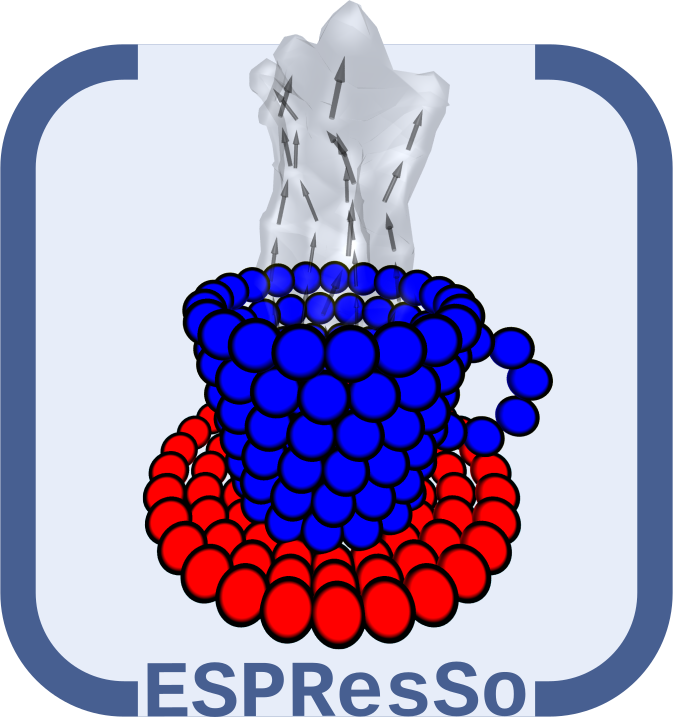
\includegraphics[width=5cm]{logo.jpg}
  \end{center}
}
%\subject{Dissertation}
\title{\es{} User's Guide}
%\author{Dipl.-Inform. Olaf~Lenz}
%\date{\today}
\maketitle

\tableofcontents

\chapter{Introduction}
\label{chap:intro}

(new)

\begin{itemize}
\item \es{} is a generic soft matter simulation packages
\item for molecular dynamics simulations in soft matter research
\item focussed on coarse-grained models
\item employs modern algorithms (Lattice-Boltzmann, DPD, P3M, \ldots)
\item written in C for maximal portability
\item Tcl-controlled
\item parallelized
\end{itemize}

\section{Guiding principles}
\label{sec:ideas}

(from paper: 2.1 Goals and principles)

\es
\begin{itemize}
\item does \emph{not} do the physics for you!
\item requires you to understand what you do (can not be used as a
  black box)
\item gives you maximal freedom (flexibility)
\item is extensible
\item integrates system setup, simulation and analysis, as this can't
  be strictly separated in soft matter simulations
\item has no predefined units
\item sets as few defaults as possible
\end{itemize}

\section{Algorithms contained in \es}

The following algorithms are implemented in \es{}:

\begin{itemize}
\item ensembles: NVE, NVT, NpT
\item charged systems:
  \begin{itemize}
  \item P3M for fully periodic systems
  \item ELC and MMM-family of algorithms for charged systems with
    non-periodic boundary conditions
  \item Maggs algorithm 
  \end{itemize}
\item Hydrodynamics:
  \begin{itemize}
  \item DPD (as a thermostat)
  \item Lattice-Boltzmann
  \end{itemize}
\end{itemize}

\section{Basic program structure}
\label{sec:structure}

(from paper: 2.2 Basic program structure)

\begin{itemize}
\item Control level: \texttt{Tcl}
\item ``Kernel'' written in \texttt{C}
\item This manual will focus on the control level
\end{itemize}

\section{On units}
\label{sec:units}

(new)

\begin{itemize}
\item Reduced units
\item comparison to ``real units''
\item three examples on different length scales
  \begin{itemize}
  \item some atomistic model?
  \item coarse-grained model (\eg lipid bilayer)
  \item billards?
  \end{itemize}
\end{itemize}

\chapter{Installation}
\label{chap:install}
\index{Installation|textbf}

\begin{itemize}
\item Compiling \es{} is a necessary evil
\item Features can be compiled in or not
\item For maximal efficiency, compile in only the features that you
  use
\item \es{} can be obtained from the \es{} home page
  \footnote{\url{http://www.espresso.mpg.de}}.
\end{itemize}

\section{Requirements}
\label{sec:requirements}
\index{requirements}

\begin{description}
\item[Tcl/Tk] \index{Tcl/Tk} \es{} requires the Toolkit Command
  Language Tcl/Tk \footnote{\url{http://www.tcl.tk/}} in the version
  8.3 or later.  Some example scripts will only work with Tcl 8.4. You
  do not only need the interpreter, but also the header files and
  libraries.  Depending on the operating system, these may come in
  separate development packages. If you want to use a graphical user
  interface (GUI) for your simulation scripts, you will also need Tk.
  
\item[FFTW] \index{FFTW} In addition, \es{} needs the FFTW library
  \footnote{\url{http://www.fftw.org/}} for Fourier transforms.
  ESPResSo can work with both the 2.1.x and 3.0.x series. Again, the
  header files are required.
  
\item[MPI] \index{MPI} Finally, if you want to use \es{} in parallel,
  you need a working MPI environment (version 1.2). Currently, the
  following MPI implementations are supported:
  \begin{itemize}
  \item LAM/MPI is the preferred variant
  \item MPICH, which seems to be considerably slower than LAM/MPI in
    our benchmarks.
  \item On AIX systems, \es{} can also use the native POE parallel
    environment.
  \item On DEC/Compaq/HP OSF/Tru64, \es{} can also use the native
    dmpirun MPI environment.
  \end{itemize}
\end{description}

\section{Quick start}

\index{configure}\index{make}

In many cases, to compile \es{}, it is enough to execute the following
sequence of two steps in the directory where you have unpacked the
sources:
\begin{verbatim}
> configure
> make
\end{verbatim}

In some cases, \eg{} when \es{} needs to be compiled for several
different platforms or when different versions with different sets of
features are required, it might be useful to execute the commands not
in the source directory itself, but to start \texttt{configure} from
another directory (see section \vref{sec:builddir}). Furthermore, many
features of \es{} can be selectively turned on or off in the local
configuration header of \es{} (see section \vref{sec:myconfig}) before
starting the compilation with \texttt{make}.

The shell script \texttt{configure} prepares the source code for
compilation. It will determine how to use and where to find the
different libraries and tools required by the compilation process, and
it will test what compiler flags are to be used.  The script will find
out most of these things automatically.  If something is missing, it
will complain and give hints how to solve the problem.  The
configuration process can be controlled with the help of a number of
options that are explained in section \vref{sec:configure}.

The command \texttt{make} will compile the source code. Depending on
the options passed to the program, \texttt{make} can also be used for
a number of other things:
\begin{itemize}
\item It can install and uninstall the program to some other
  directories. However, normally it is not necessary to actually
  \textit{install} \es{} to run it.
\item It can test the \es{} program for correctness.
\item It can build the documentation.
\end{itemize}
The details of the usage of \texttt{make} are described in section
\vref{sec:make}.

When these steps have successfully completed, \es{} can be started
with the command (see section \vref{sec:run})
\begin{verbatim}
> Espresso
\end{verbatim}

\section{Source and build directory}
\label{sec:builddir}
\index{build directory} \index{source directory}

If you plan to use \es{} with a single configuration, you can skip the
rest of this section. If then you have problems finding the \es{}
binary or you come upon a reference to the \emph{build directory} in
the documentation, you might have to read it, anyway. 

Usually, when a program is compiled, the resulting binary files are
put into the same directory as the sources of the program. In \es{},
the \emph{source directory} that contains all the source files can be
completely separated from the \emph{build directory} where the files
created by the build process are put. As the source directory is not
touched during the compilation process, it is possible to compile more
than one binary version of \es{} from the same set of source files.
This is useful in cases when \es{} is to be used on different computer
hardware or with a different configuration.

The source directory is the directory that contains the source files.
The location of the build directory is determined when the
\texttt{configure}-script is called.  Usually, the build directory is
assigned to the current working directory when the
\texttt{configure}-script was called. All further commands concerning
compiling and running \es{} have to be called from this directory.

\paragraph{Example}
When the source directory is \texttt{\$srcdir} (\ie{} the files where
unpacked to this directory), then the build directory can be set to
\texttt{\$builddir} by calling the \texttt{configure}-script from
there:
\begin{verbatim}
> cd $builddir
> $srcdir/configure
> make
> Espresso
\end{verbatim}

When \texttt{configure} is called directly from the source directory,
the \es{} build system is prepared to handle different platforms.  A
new subdirectory is created and \texttt{configure} is recursively
called from this directory, making the subdirectory the build
directory.  The directory is called
\texttt{obj-}\textit{platform}\texttt{/}, where \textit{platform} is a
descriptor of the CPU type where the script was started, \eg{}
\texttt{obj-Athlon\_64-pc-linux}.

In this case it is also possible to run the commands \texttt{make} and
\texttt{Espresso} directly in the source directory.

Furthermore, the option \texttt{--enable-chooser} will be set in the
recursive call of \texttt{configure} that activates the automatic
binary chooser (see section \vref{sec:install_dir}).

\section{Installation directories}
\label{sec:install_dir}

Normally, the \es-binary \texttt{Espresso-bin} is installed in the
directory \texttt{\$prefix/libexec/} and a the wrapper script
\texttt{Espresso} in the directory \texttt{\$prefix/bin/} that handles
the MPI invocation.

When the \texttt{configure}-script is called from the source directory
or when the option \texttt{--enable-chooser} is given, an automatic
binary chooser is installed in the directory \texttt{\$prefix/bin/}
and the \es{}-binary and the MPI wrapper script are installed in an
architecture-specific subdirectory
\mbox{\texttt{\$exec-prefix/lib/espresso/obj-}\textit{platform}\texttt{/}}.
When called, the binary chooser will automatically call the MPI
wrapper script in the right subdirectory.

\section{The configuration header \texttt{myconfig.h}}
\label{sec:myconfig}

\index{myconfig.h} \index{configuration header} \es{} has a great
number of features that can be compiled into the binary (see chapter
\vref{chap:features}).  However, it is not recommended to actually
compile in all possible features, as this will negatively affect \es's
performance. Instead, compile in only the features that are actually
required. For the developers, it is also possible to turn on or off a
number of debugging messages. The features and debug messages can be
controlled via a configuration header file that contains
C-preprocessor declarations. See Sec.\ref{sec:configflags} for possible
declarations.

By default, the configuration header is called \texttt{myconfig.h}.
The name of the configuration header can be either changed when the
\texttt{configure}-script is called with the option
\texttt{--with-myconfig} (see section \vref{sec:configure}), or when
\texttt{make} is called with the setting
\texttt{myconfig=}\textit{myconfig\_header} (see section
\vref{sec:make}).

The configuration header can be put in the build directory, or in the
source directory. When a configuration header is found in both
directories, the one in the build directory will be used. If both
directories do not contain a configuration header, a default header
will be used that turns on the default features.

The file \texttt{myconfig-sample.h} in the source directory contains
an example configuration header.

\paragraph{Example}
The configuration header can be used to compile different versions
from the same source directory. Suppose that you have a source
directory \texttt{\$srcdir} and two build directories
\texttt{\$builddir1} and \texttt{\$builddir2} that contain different
configuration headers:

\begin{itemize}
\item \texttt{\$builddir1/myconfig.h}:
\begin{verbatim}
#define ELECTROSTATICS
#define LENNARD-JONES
\end{verbatim}

\item \texttt{\$builddir2/myconfig.h}:
\begin{verbatim}
#define LJCOS
\end{verbatim}
\end{itemize}

\noindent Then you can simply compile two different versions of \es{} via
\begin{verbatim}
cd $builddir1
$srcdir/configure
make

cd $builddir2
$srcdir/configure
make
\end{verbatim}

\section{Configuration options}
\label{sec:configflags}
\newcommand\configswitch[1]{\texttt{\bf #1}}

In \texttt{myconfig-sample.h} you can use the following general switches:
\begin{itemize}
\item \configswitch{PARTIAL\_PERIODIC} By default, all coordinates in \es{} are periodic. With
  \texttt{PARTIAL\_PERIODIC} turned on, the \es{} global variable \texttt{periodic} (see
  Sec.~\ref{sec:globalvar}) controls the periodicity of the individual coordinates. Note that this
  slows the integrator down by around $10-30\%$.
\item \configswitch{ELECTROSTATICS} This switches on the various electrostatics algorithms, such as
  the Ewald summation. See Sec.~\ref{sec:electrostatics} for details on this algorithms.
\item \configswitch{ROTATION} Switch on rotational degrees of freedom for the particles, as well as
  the corresponding quaternion integrator. See Sec.~\ref{sec:rotation} for details.
\item \configswitch{DIPOLES} This activates the dipole support in P$^3$M. Currently, a mixing of
  dipoles and charges is not possible, i.~e. all particles have to have charge $q=0$.
  Requires \texttt{ELECTROSTATICS} and \texttt{ROTATION}.
\item \configswitch{EXTERNAL\_FORCES} Allows to define an arbitrary constant force for each particle
  individually. Also allows to fix individual coordinates of particles, e.~g. keep them at a fixed
  position or within a plane.
\item \configswitch{CONSTRAINTS} Turns on various spatial constraints such as spherical compartments
  or walls. This constraints interact with the particles through regular short ranged potentials
  such as the Lennard--Jones potential. See Sec.~\ref{sec:constraints} for possible constraint
  forms.
\item \configswitch{MASS} Allows particles to have individual masses. Note that some analyzation
  procedures have not yet been adapted to take the masses into account correctly.
\item \configswitch{EXCLUSIONS} Allows to exclude specific short ranged interactions within
  molecules, which is necessary for some atomistic models.
\item \configswitch{COMFORCE}
\item \configswitch{COMFIXED}
\item \configswitch{MOLFORCES}
\item \configswitch{BOND\_CONSTRAINT} Turns on the RATTLE integrator which allows for fixed lengths
  bonds between particles.
\end{itemize}

In addition, there are switches that enable additional features in the integrator:
\begin{itemize}
\item \configswitch{NEMD} Enables the non-equilbrium (shear) MD support (see Sec.~\ref{sec:NEMD}).
\item \configswitch{NPT} Enables an on--the--fly NPT integration scheme (see Sec.~\ref{sec:NPT}).
\item \configswitch{DPD} Enables the dissipative particle dynamics thermostat (see
  Sec.~\ref{sec:DPD}).
\item \configswitch{LB} Enables the lattice-Boltzmann fluid code (see Sec.~\ref{sec:LB}).
\end{itemize}

\subsection{Switches for interactions}
The following switches turn on various short ranged interactions (see Sec.~\ref{sec:shortrange}):
\begin{itemize}
\item \configswitch{TABULATED} Enable support for user--defined interactions, e.~g. for atomistic
  simulations.
\item \configswitch{LENNARD\_JONES} Enable the Lennard--Jones potential.
\item \configswitch{LJ\_WARN\_WHEN\_CLOSE} This adds an additional check to the Lennard--Jones
  potential that prints a warning of particles come too close so that the simulation becomes
  unphysical.
\item \configswitch{MORSE} Enable the Morse potential.
\item \configswitch{LJCOS} Enable the Lennard--Jones potential with a cosine--tail.
\item \configswitch{LJCOS2}
\item \configswitch{BUCKINGHAM} Enable the Buckingham potential.
\item \configswitch{SOFT\_SPHERE} Enable the soft sphere potential.
\end{itemize}

If you want to use angle bonds, you currently need to choose the type a priory (see
Sec.~\ref{sec:angle}). This will change in the near future to three independent angle potentials:
\begin{itemize}
\item \item \configswitch{BOND\_ANGLE\_HARMONIC}
\item \configswitch{BOND\_ANGLE\_COSINE}
\item \configswitch{BOND\_ANGLE\_COSSQUARE}
\end{itemize}

\subsection{Debug--switches}
Finally, there are a number of flags for debugging. The most important one are
\begin{itemize}
\item \configswitch{ADDITIONAL\_CHECKS} Enables numerous additional checks which can detect
  inconsistencies especially in the cell systems. This checks are however too slow to be enabled in
  production runs.
\item \configswitch{MEM\_DEBUG} Enables an internal memory allocation checking system. This produces
  output for each allocation and freeing of a memory chunk, and therefore allows to track down
  memory leaks. This works by internally replacing \texttt{malloc}, \texttt{realloc} and
  \texttt{free}.
\end{itemize}

The following flags control the debug output of various sections of Espresso. You will however
understand the output very often only by looking directly at the code.
\begin{itemize}
\item \configswitch{COMM\_DEBUG} Output from the asynchronous communication code.
\item \configswitch{EVENT\_DEBUG} Notifications for event calls, i.~e. the \texttt{on\_?} functions
  in \texttt{initialize.c}. Useful if some module does not correctly respond to changes of e.~g.
  global variables.
\item \configswitch{INTEG\_DEBUG} Integrator output.
\item \configswitch{CELL\_DEBUG} Cellsystem output.
\item \configswitch{GHOST\_DEBUG} Cellsystem output specific to the handling of ghost cells and the
  ghost cell communication.
\item \configswitch{GHOST\_FORCE\_DEBUG}
\item \configswitch{VERLET\_DEBUG} Debugging of the Verlet list code of the domain decomposition cell
  system.
\item \configswitch{LATTICE\_DEBUG} Universal lattice structure debugging.
\item \configswitch{HALO\_DEBUG}
\item \configswitch{GRID\_DEBUG}
\item \configswitch{PARTICLE\_DEBUG} Output from the particle handling code.
\item \configswitch{P3M\_DEBUG}
\item \configswitch{ESR\_DEBUG} debugging of P$^3$Ms real space part.
\item \configswitch{ESK\_DEBUG} debugging of P$^3$Ms $k$--space part.
\item \configswitch{EWALD\_DEBUG}
\item \configswitch{FFT\_DEBUG} Output from the unified FFT code.
\item \configswitch{MAGGS\_DEBUG}
\item \configswitch{RANDOM\_DEBUG}
\item \configswitch{FORCE\_DEBUG} Output from the force calculation loops.
\item \configswitch{THERMO\_DEBUG} Output from the thermostats.
\item \configswitch{LJ\_DEBUG} Output from the Lennard--Jones code.
\item \configswitch{MORSE\_DEBUG} Output from the Morse code.
\item \configswitch{FENE\_DEBUG}
\item \configswitch{ONEPART\_DEBUG} Define to a number of a particle to obtain output on the forces
  calculated for this particle.
\item \configswitch{STAT\_DEBUG}
\item \configswitch{POLY\_DEBUG}
\item \configswitch{MOLFORCES\_DEBUG}
\item \configswitch{LB\_DEBUG} Output from the lattice--Boltzmann code.
\item \configswitch{ASYNC\_BARRIER} Introduce a barrier after each asynchronous command
  completion. Helps in detection of mismatching communication.
\item \configswitch{FORCE\_CORE} Causes \es{} to try to provoke a core dump when exiting
  unexpectedly.
\item \configswitch{MPI\_CORE} Causes \es{} to try this even with MPI errors.
\end{itemize}

\section{Running configure}
\label{sec:configure}

\index{configure}
The shell script \texttt{configure} collects all the information
required by the compilation process. It will determine how to use and
where to find the different libraries and tools required by the
compilation process, and it will test what compiler flags are to be
used.  The script will find out most of these things automatically.
If something is missing, it will complain and give hints how to solve
the problem.

The generic syntax of calling the \texttt{configure} script is:
\begin{syntax}
 $>$ configure [\var{options} ...] [\var{variable}=\var{value} ...]
\end{syntax}

\index{configure options}
The behaviour of \texttt{configure} can be controlled by the means of
command line options. In the following, only those command line
options that are special to \es{} will be explained.  For a complete
list of options and explanations thereof, call
\begin{verbatim}
> configure --help
\end{verbatim}

\begin{description}
\item [\texttt{--enable-chooser}] This option will enable the
  automatic choosing mechanism for \es{} (see section
  \vref{sec:install_dir}).  This option will be automatically enabled,
  when the \texttt{configure} script is called from the source
  directory, otherwise it will be disabled. It is not recommended to
  set the option manually.
\item[\texttt{--enable-config=KNOWN\_CONFIG}] For some known systems,
  where \texttt{configure} does not find the required libraries and
  compiler options, predefined settings can be used. The following
  configuration names are known: \texttt{dino} and \texttt{blade}. The
  default for this option is: \texttt{none}.
\item[\texttt{--enable-debug}] This option will enable compiler flags
  required for debugging \es{} and is disabled by default.
\item[\texttt{--enable-profiling}] This option will enable compiler
  flags required for profiling \es{} and is disabled by default.
\item[\texttt{--disable-processor-optimization}] This option will
  control whether \texttt{configure} will check for several
  optimization flags to be used by the compiler. This option is
  enabled by default.
\item[\texttt{--enable-xlc-qipa}] This option is only useful when the
  IBM C-compiler \texttt{xlc} is used and will control whether or not
  the compiler flag \texttt{-qipa} is used. This option is enabled by
  default.

\item[\texttt{--with-myconfig=MYCONFIG\_HEADER}] This option sets the
  name of the local configuration header (see \vref{sec:myconfig}). It
  defaults to ``\texttt{myconfig.h}''.
\item[\texttt{--with-mpi=MPI}] Sets the MPI implementation that should
  be used. By default, \texttt{configure} will test autoamtically what
  MPI implementation is available. The following implementations are
  known: 
  \begin{description}
  \item[\texttt{fake}, \texttt{no}] This will disable MPI completely.
  \item[\texttt{lam}] Use the LAM/MPI environment
    (\url{http://www.lam-mpi.org/}).
  \item[\texttt{mpich}] Use the MPICH environment
    (\url{http://www-unix.mcs.anl.gov/mpi/mpich/}).
  \item[\texttt{poe}] Use the POE environment (IBM).
  \item[\texttt{dmpi}] Use the DMPI environment (Tru64).
  \item[\texttt{generic}] Use a generic MPI implementation. This will
    try to find an MPI compiler and an MPI runtime environment.
  \end{description}
\item[\texttt{--with-efence}] Whether or not to use the ``electric
  fence'' memory debugging library
  (\url{http://freshmeat.net/projects/efence/}). Efence is not used by
  default.
\item[\texttt{--with-tcl=TCL}] When the wrong version of the Tcl
  library is used by configure, the name of the Tcl-library can be
  specified with this option, \eg{} \texttt{tcl8.4}.
\item[\texttt{--with-tk=TK}] By default, the GUI toolkit Tk is not
  used by \es. This option can be used to activate Tk and to specify
  which Tk version to use, \eg{} \texttt{tk8.4}.
\item[\texttt{--with-fftw=VERSION}] This can be used to specify which
  version of fftw is to be used. By default, version 3 will be used if
  it is found, otherwise version 2 is used.
\end{description}

\section{Compiling, testing and installing \es}
\label{sec:make}

The command \texttt{make} is mainly used to compile the \es{} source
code, but it can do a number of other things. The generic syntax of
the \texttt{make} command is:
\begin{syntax}
 $>$ make [\var{target}...] [\var{variable}=\var{value}]
\end{syntax}
When no target is given, the target \texttt{all} is used. The
following targets are available:
\begin{description}
\item[\texttt{all}] Compiles the complete \es{} source code.
\item[\texttt{check}] Runs the testsuite. By default, all available
  tests will be run on 1, 2, 3, 4, 6, or 8 processors. Which tests are
  run can be controlled by means of the variable \texttt{tests}, which
  processor numbers are to be used can be controlled via the variable
  \texttt{processors}. Note that depending on your MPI installation,
  MPI jobs can only be run in the queueing system, so that \es{} will
  not run from the command line. In that case, you may not be able to
  run the testsuite, or you have to directly submit the testsuite script
  \verb!testsuite/test.sh! to the queueing system.\\
  \textbf{Example:} \verb!make check tests="madelung.tcl" processors="1 2"!\\
  will run the test \texttt{madlung.tcl} on one and two processors.
\item[\texttt{clean}] Deletes all files that were created furing the
  compilation.
\item[\texttt{mostlyclean}] Deletes most files that were created
  during the compilation. Will keep for example the built doxygen
  documentation and the \es{} binary.
\item[\texttt{dist}] Creates a \texttt{.tar.gz}-file of the \es{}
  sources.  This will include all source files as they currently are
  in the source directory, \ie{} it will include local changes.  This
  is useful to give your version of \es{} to other people.
  The variable \texttt{extra} can be used to specify additional
  files and directories that are to be included in the archive
  file. \\
  \textbf{Example:} \verb!make dist extra="myconfig.h internal"!\\
  will create the archive file and include the file
  \texttt{myconfig.h} and the directory \texttt{internal} with all
  files and subdirectories.
\item[\texttt{install}] Install \es{}. The variables \texttt{prefix}
  and \texttt{exec-prefix} can be used to specify the installation
  directories, otherwise the defaults defined by the
  \texttt{configure} script are used. \texttt{prefix} sets the basic
  prefix where all \es{} files are to be installed,
  \texttt{exec-prefix} sets the prefix where the executable files are
  to be installed and is required only when there is an
  architecture-specific directory.\\
  \textbf{Example:} \verb!make install prefix=/usr/local!\\
  will install all files below \texttt{/usr/local}.
\item[\texttt{uninstall}] Uninstalls \es{}, \ie{} removes all files
  that were installed during \texttt{make install}. The variables are
  identical to the variables of the \texttt{install}-target.
\end{description}

\section{Running \es}
\label{sec:run}

\es{} can be run via
\begin{syntax}
$>$ Espresso [\var{tcl\_script} [\var{N\_processors} [\var{args}]]]
\end{syntax}

\index{interactive mode} When \es{} is called without any arguments,
it is started in the interactive mode, where new commands can be
entered on the command line. When the name of a \textit{tcl\_script}
is given, the script is executed. \textit{N\_processors} is the number
of processors that are to be used. Any further arguments are passed to
the script. Note that depending on your MPI installation, MPI jobs can
only be run in the queueing system, so that \es{} will not run from
the command line.

% A number of wrapper scripts are used in running \es{}:
% \begin{itemize}
% \item The script \texttt{Espresso} in the source and build directory
%   will try to run the compiled version of \es. If it is called from
%   the source directory, it assumes that \es{} was also configured in
%   the source directory and will try to recursively start the script in
%   the corresponding \texttt{obj-PLATFORM} build directory. If it is
%   called in the build directory, it will start the \es-binary with the
%   right MPI implementation.
% \item The chooser script \texttt{Espresso} 
%   \begin{itemize}
%   \item installed when \verb!--enable-chooser! was given
%   \item installed to bindir
%   \item tries to run the correct version of the MPI-wrapper
%     \texttt{Espresso}
%   \end{itemize}
% \item The MPI-wrapper \texttt{Espresso}
%   \begin{itemize}
%   \item installed next to \es{} binary
%   \item starts the binary with the right MPI implementation
%   \end{itemize}
% \item The \es{} binary \texttt{Espresso-bin} can also be started
%   directly, however, it requires that the environment variable
%   \verb!ESPRESSO_SCRIPTS! is set to the directory where the scripts
%   are installed (usually \verb!$(prefix)/lib/espresso/scripts! or
%   \verb!$(prefix)/share/espresso/scripts!).
% \end{itemize}



%%% Local Variables: 
%%% mode: latex
%%% TeX-master: "ug"
%%% End: 


\chapter{Tutorial}
\label{chap:tutorial}

(from \verb!erice_tutorial! or appendix A from paper)

\begin{itemize}
\item \es: script interpreter
\item interactive use (sample session)
\item script execution
\item example script
\item Reference to \verb!tutorial.tcl! (?)
\end{itemize}

\chapter{\es{} command reference}
\label{chap:ref}

(most from paper and from related pages)

\begin{itemize}
\item Will contain description of all Tcl-commands
\item Reference to appendix \vref{chap:quickref}
\item basic identifiers:
  \begin{itemize}
  \item particle type
  \item bonded interaction type
  \item molecule id
  \end{itemize}
\end{itemize}


\section{\texttt{inter}: Setting up interactions}
\label{sec:inter}
\begin{syntax}
  \variant{1}
  {inter 
    \var{part\_type\_id1} 
    \var{part\_type\_id2}
    \var{inter\_type} 
    [ \var{parameters}\ldots ]
  }
  \variant{2}
  {inter 
    \var{bond\_type\_id} \var{bond\_type} [
    \var{parameters}\ldots ]
  }
  \variant{3}
  {inter}
\end{syntax}
    % \section{Creating particles}
% \label{sec:part}
% \texttt{part}

% \section{Interactions}
% \label{sec:inter}
% \texttt{inter}

% \section{Analysis}
% \label{sec:analysis}

\chapter{Under the hood}
\label{chap:underhood}

(new)

\begin{itemize}
\item Implementation issues that are interesting for the user
\item Main loop in pseudo code (for comparison)
\item from doxygen: ``Cell systems'' 
\end{itemize}


\chapter{Getting involved}
\label{chap:devel}

\begin{itemize}
\item What to do when you want to become involved
\item How to submit a bug report
\end{itemize}


\appendix
\chapter{\es{} quick reference}
\label{chap:quickref}

\begin{itemize}
\item Short reference table of all commands
\item Complete syntax of \es{} commands
\item Features required for different commands
\end{itemize}

\chapter{The MMM family of algorithms}
\label{chap:mmm}

\chapter{Maggs algorithm}
\label{chap:maggs}

\end{document}


%%% Local Variables: 
%%% mode: latex
%%% TeX-master: t
%%% End: 

%\listofcommands

%%% Local Variables: 
%%% mode: latex
%%% TeX-master: "ug"
%%% End: 

\chapter{Features}
\label{sec:features}
\index{features|textbf}

\newcommand{\feature}[1]{\texttt{\textbf{#1}}}

This chapter describes the features that can be activated in \es. Even
if possible, it is not recommended to activate all features, because
this will negatively effect \es's performance.

Features can be activated in the configuration header (see section
\vref{sec:myconfig}). Too activate \texttt{FEATURE}, add the following
line to the header file:
\begin{verbatim}
#define FEATURE
\end{verbatim}

\subsection{General features}
\begin{itemize}
\item \feature{PARTIAL\_PERIODIC} By default, all coordinates in \es{} are periodic. With
  \texttt{PARTIAL\_PERIODIC} turned on, the \es{} global variable \texttt{periodic} (see
  Sec.~\ref{sec:globalvar}) controls the periodicity of the individual coordinates. Note that this
  slows the integrator down by around $10-30\%$.
\item \feature{ELECTROSTATICS} This switches on the various electrostatics algorithms, such as
  the Ewald summation. See Sec.~\ref{sec:electrostatics} for details on this algorithms.
\item \feature{ROTATION} Switch on rotational degrees of freedom for the particles, as well as
  the corresponding quaternion integrator. See Sec.~\ref{sec:rotation} for details.
\item \feature{DIPOLES} This activates the dipole support in P$^3$M. Currently, a mixing of
  dipoles and charges is not possible, i.~e. all particles have to have charge $q=0$.
  Requires \texttt{ELECTROSTATICS} and \texttt{ROTATION}.
\item \feature{EXTERNAL\_FORCES} Allows to define an arbitrary constant force for each particle
  individually. Also allows to fix individual coordinates of particles, e.~g. keep them at a fixed
  position or within a plane.
\item \feature{CONSTRAINTS} Turns on various spatial constraints such as spherical compartments
  or walls. This constraints interact with the particles through regular short ranged potentials
  such as the Lennard--Jones potential. See Sec.~\ref{sec:constraints} for possible constraint
  forms.
\item \feature{MASS} Allows particles to have individual masses. Note that some analyzation
  procedures have not yet been adapted to take the masses into account correctly.
\item \feature{EXCLUSIONS} Allows to exclude specific short ranged interactions within
  molecules, which is necessary for some atomistic models.
\item \feature{COMFORCE}
\item \feature{COMFIXED}
\item \feature{MOLFORCES}
\item \feature{BOND\_CONSTRAINT} Turns on the RATTLE integrator which allows for fixed lengths
  bonds between particles.
\end{itemize}

In addition, there are switches that enable additional features in the integrator:
\begin{itemize}
\item \feature{NEMD} Enables the non-equilbrium (shear) MD support (see Sec.~\ref{sec:NEMD}).
\item \feature{NPT} Enables an on--the--fly NPT integration scheme (see Sec.~\ref{sec:NPT}).
\item \feature{DPD} Enables the dissipative particle dynamics thermostat (see
  Sec.~\ref{sec:DPD}).
\item \feature{LB} Enables the lattice-Boltzmann fluid code (see Sec.~\ref{sec:LB}).
\end{itemize}

\subsection{Interactions}
The following switches turn on various short ranged interactions (see Sec.~\ref{sec:shortrange}):
\begin{itemize}
\item \feature{TABULATED} Enable support for user--defined interactions, e.~g. for atomistic
  simulations.
\item \feature{LENNARD\_JONES} Enable the Lennard--Jones potential.
\item \feature{LJ\_WARN\_WHEN\_CLOSE} This adds an additional check to the Lennard--Jones
  potential that prints a warning of particles come too close so that the simulation becomes
  unphysical.
\item \feature{MORSE} Enable the Morse potential.
\item \feature{LJCOS} Enable the Lennard--Jones potential with a cosine--tail.
\item \feature{LJCOS2}
\item \feature{BUCKINGHAM} Enable the Buckingham potential.
\item \feature{SOFT\_SPHERE} Enable the soft sphere potential.
\end{itemize}

If you want to use angle bonds, you currently need to choose the type
a priori (see section \vref{sec:angle}). This will change in the near
future to three independent angle potentials:
\begin{itemize}
\item \feature{BOND\_ANGLE\_HARMONIC}
\item \feature{BOND\_ANGLE\_COSINE}
\item \feature{BOND\_ANGLE\_COSSQUARE}
\end{itemize}

\subsection{Debug messages}
Finally, there are a number of flags for debugging. The most important one are
\begin{itemize}
\item \feature{ADDITIONAL\_CHECKS} Enables numerous additional checks which can detect
  inconsistencies especially in the cell systems. This checks are however too slow to be enabled in
  production runs.
\item \feature{MEM\_DEBUG} Enables an internal memory allocation checking system. This produces
  output for each allocation and freeing of a memory chunk, and therefore allows to track down
  memory leaks. This works by internally replacing \texttt{malloc}, \texttt{realloc} and
  \texttt{free}.
\end{itemize}

The following flags control the debug output of various sections of Espresso. You will however
understand the output very often only by looking directly at the code.
\begin{itemize}
\item \feature{COMM\_DEBUG} Output from the asynchronous communication code.
\item \feature{EVENT\_DEBUG} Notifications for event calls, i.~e. the \texttt{on\_?} functions
  in \texttt{initialize.c}. Useful if some module does not correctly respond to changes of e.~g.
  global variables.
\item \feature{INTEG\_DEBUG} Integrator output.
\item \feature{CELL\_DEBUG} Cellsystem output.
\item \feature{GHOST\_DEBUG} Cellsystem output specific to the handling of ghost cells and the
  ghost cell communication.
\item \feature{GHOST\_FORCE\_DEBUG}
\item \feature{VERLET\_DEBUG} Debugging of the Verlet list code of the domain decomposition cell
  system.
\item \feature{LATTICE\_DEBUG} Universal lattice structure debugging.
\item \feature{HALO\_DEBUG}
\item \feature{GRID\_DEBUG}
\item \feature{PARTICLE\_DEBUG} Output from the particle handling code.
\item \feature{P3M\_DEBUG}
\item \feature{ESR\_DEBUG} debugging of P$^3$Ms real space part.
\item \feature{ESK\_DEBUG} debugging of P$^3$Ms $k$--space part.
\item \feature{EWALD\_DEBUG}
\item \feature{FFT\_DEBUG} Output from the unified FFT code.
\item \feature{MAGGS\_DEBUG}
\item \feature{RANDOM\_DEBUG}
\item \feature{FORCE\_DEBUG} Output from the force calculation loops.
\item \feature{THERMO\_DEBUG} Output from the thermostats.
\item \feature{LJ\_DEBUG} Output from the Lennard--Jones code.
\item \feature{MORSE\_DEBUG} Output from the Morse code.
\item \feature{FENE\_DEBUG}
\item \feature{ONEPART\_DEBUG} Define to a number of a particle to obtain output on the forces
  calculated for this particle.
\item \feature{STAT\_DEBUG}
\item \feature{POLY\_DEBUG}
\item \feature{MOLFORCES\_DEBUG}
\item \feature{LB\_DEBUG} Output from the lattice--Boltzmann code.
\item \feature{ASYNC\_BARRIER} Introduce a barrier after each asynchronous command
  completion. Helps in detection of mismatching communication.
\item \feature{FORCE\_CORE} Causes \es{} to try to provoke a core dump when exiting
  unexpectedly.
\item \feature{MPI\_CORE} Causes \es{} to try this even with MPI errors.
\end{itemize}

%%% Local Variables: 
%%% mode: latex
%%% TeX-master: "ug"
%%% End: 

% Copyright (C) 2010,2012,2013 The ESPResSo project
% Copyright (C) 2002,2003,2004,2005,2006,2007,2008,2009,2010 
%   Max-Planck-Institute for Polymer Research, Theory Group
%  
% This file is part of ESPResSo.
%   
% ESPResSo is free software: you can redistribute it and/or modify it
% under the terms of the GNU General Public License as published by the
% Free Software Foundation, either version 3 of the License, or (at your
% option) any later version.
%  
% ESPResSo is distributed in the hope that it will be useful, but
% WITHOUT ANY WARRANTY; without even the implied warranty of
% MERCHANTABILITY or FITNESS FOR A PARTICULAR PURPOSE.  See the GNU
% General Public License for more details.
%  
% You should have received a copy of the GNU General Public License
% along with this program.  If not, see <http://www.gnu.org/licenses/>.
%
\chapter{Sample scripts}
\label{chap:samples}

In the directory \es{}/samples you find several scripts that can serve
as samples how to use \es{}.
\begin{description}
\item[lj\_liquid.tcl] Simple Lennard-Jones particle liquid. Shows the
  basic features of \es: How to set up system parameters, particles
  and interactions. How to warm up and integrate. How to write
  parameters, configurations and observables to files. How to handle
  the connection to VMD.
%\item[kremerGrest.tcl] This reproduces the data of \citet{kremer90a}:
%  Multiple systems with different number of neutral polymer chains of
%  various lengths are simulated for very long times at melt density
%  0.85 while their static and some dynamic properties are measured.
%  Shows the advanced features of \es{}: How to run several simulations
%  from a single script. How to use online-analysis (The analyze
%  command) with comparision to expectation values. How to get averages
%  of the observables. How to set/restore checkpoints (Using
%  Checkpoints, saving configurations) including auto-detection of
%  previously derived parts of the simulation(s). How to create
%  gnuplots from within the script and combine multiple plots onto
%  duplex pages (Statistical Analysis and Creating Gnuplots).  In the
%  end the script will provide plots of all important quantities as
%  .ps- and .pdf-files while compressing the data-files. Note however,
%  that the simulation uses the original time scale, hence it may take
%  quite some time to finish.
\item[pe\_solution.tcl] Polyelectrolyte solution under poor solvent
  condition. Test case for comparison with data produced by polysim9
  from M.Deserno. Note that the equilibration of this system takes
  roughly $15000 \tau$.
\item[pe\_analyze.tcl] Example for doing the analysis after the actual
  simulation run (offline analysis). Calculates the integrated ion
  distribution $P(r)$ for several different time slaps, compares them
  and presents the final result using gnuplot to generate some
  ps-files.
\item[harmonic\_oscillator.tcl] A chain of harmonic oscillators. This
  is a $T=0$ simulation to test the energy conservation.
\item[espresso\_logo.tcl] The \es-logo, the exploding espresso cup,
  has been created with this script. It is a regular simulation of a
  polyelectrolyte solution. It makes use of some nice features of the
  part command (see section \vref{tcl:part}, namely the capability to
  fix a particle in space and to apply an external force.
\end{description}

%%% Local Variables: 
%%% mode: latex
%%% TeX-master: "ug"
%%% End: 


%% Scientific appendices: description of algorithms
\documentclass[a4paper, 12pt]{article}
\usepackage[dvips]{graphicx}
\newcommand{\vect}[1]{\mathbf{#1}}
\newcommand{\curl}[1]{\vect{\nabla}\times\vect{#1}}
\newcommand{\diverg}[1]{\vect{\nabla}\cdot\vect{#1}}
\newcommand{\partderiv}[2]{\frac{\partial{#1}}{\partial{#2}}}
\newcommand{\volumeint}{\int d^3\vect r\,}
\def\es{{\sf ESPResSo}}             % Espresso sign
\begin{document}
{\huge{\bf Coulomb Interactions via Local Dynamics: \\
A Molecular--Dynamics Algorithm}}\\
\vspace{0.2cm}
{\bf {\large Igor Pasichnyk\\
Max-Planck-Institut f\"ur Polymerforschung\\
Mainz}}
%
\section{Introduction}
%
The Molecular Dynamics method for obtaining Coulomb interactions as
the potential of mean force between charges which are dynamically
coupled to a local electromagnetic field is described. It is
intimately related to the Car--Parrinello approach, while being
equivalent to solving Maxwell's equations with freely adjustable speed
of light.
%
\section{Equations of motion}
%
Denoting the particle masses with $m_i$, their charges with $q_i$, their coordinates and momentum with $\vect
r_i$ and $\vect p_i$ respectively, the interparticle potential (of {\em non}--electromagnetic
type) with $U$,  for the coupled system of charges and fields we write the following equations of motion
%
\begin{eqnarray} 
  \dot{\vect r}_i & = & \frac{1}{m_i} \vect p_i \\
  \dot{\vect p}_i & = & - \frac{\partial U}{\partial \vect r_i} + q_i \vect E (\vect r_i)- \frac{\zeta}{m_i} \vect p_i
                        + \vect f_i \\
  \dot{\vect A} & = & - \vect E \\
  \dot{\vect E} & = & 
  c^2 \vect \nabla \times \left( \vect \nabla \times \vect A \right)
  - \frac{1}{\epsilon_0} \vect j ,
\end{eqnarray}
%
where $\epsilon_0$ is the vacuum dielectric constant, $c$ speed of light, $\vect A$ the vector-potential, $\vect E$ the elctric field, $\vect j$ the current
density; $\zeta$ is the particle friction constant, and $\vect f_i$ is a
random force satisfying the standard fluctuation--dissipation theorem:
%
\begin{equation}
\left< f_i^\alpha (t) f_j^\beta (t^\prime) \right> =
2 \zeta k_B T \delta_{ij} \delta_{\alpha \beta}
\delta (t - t^\prime),
\end{equation}
%
where $\alpha$ and $\beta$ denote Cartesian indices.

If we introduce the vector $\vect B=\curl A$ the system of equations can be rewritten in a form similar to the usual Maxwell equations. Currently in {\es} the version with $\vect B$ and $\vect E$ is implemented.
%
\section{Discretization}
%
For implementation on the computer, the equations need to be
discretized with respect to both space and time.We consider a domain of physical space as being an
affine space and divide it into subdomains of contiguous cells of
cubic shape. The charges live on the vertices of our lattice which has
the spacing $a$. The electric fields $E(l)$ and vector potentials
$A(l)$ live on the edges or links and are aligned with them. We need
also the operator $\curl{}$. It gives the vector $\vect B$, which lives on the
faces of the cube or on the plaquettes, Fig.~\ref{fig:cell_structure}.
%
\begin{figure}
  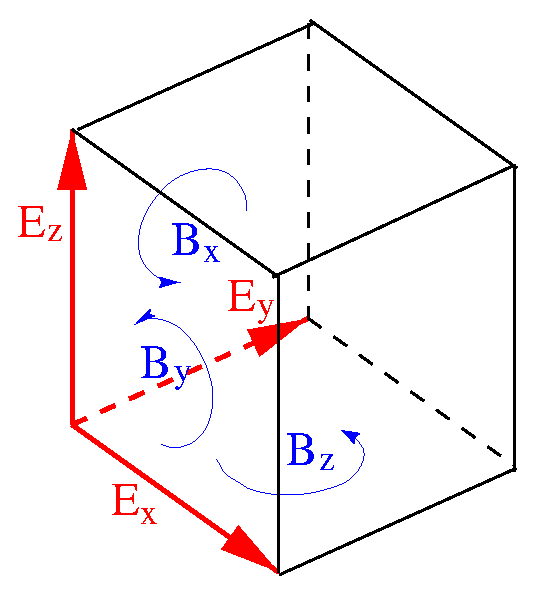
\includegraphics[scale=0.55]{figs/cell.eps}
  \caption{Spatial elements of a cell complex}
  \label{fig:cell_structure}  
\end{figure}
%
In the implementation of the algorithm we assume that particles with
masses $m_i$ live in the continuum (off--lattice approach). Particles
have charges $q_i$ and interact between themselves also by a
Lennard--Jones potential. The Lennard--Jones potential of scale $\sigma$ is 
truncated at its minimum, $r_c=2^{1/6}\sigma$. 

The charges are interpolated on the lattice
with grid spacing $a$ using the linear interpolation scheme.
%
\section{Initialization of the algorithm}
%
In order to start the simulation for the given random distribution of
charges we have to calculate the initial electrostatic field, i.~e. the
exact solution of the electrostatic problem. We find a particular solution of Gauss' law as
the result of the following recursive procedure (see
Fig.~\ref{fig:initialization_E}):
\begin{enumerate}
\item The charge in the plane $z=z_{plane}$ is 
\begin{equation}
q_{plane}=\frac{1}{N}\sum_iq(\vect r_i)\delta(z_i-z_{plane}),
\end{equation}
$N$ is the number of charges in plane $z=z_{plane}$. Update the
$z$-field according to the formula
\begin{equation}
E_z^2=E_z^1+\frac{q_{plane}}{\epsilon_0a^2};
\end{equation}
\item Subtract the
charge $q_{plane}$ from the each charge on sites of $z_{plane}$. The
charge of the wire $y=y_{wire}, z=z_{plane}$ is
\begin{equation}
q_{wire}=\frac{1}{N}\sum_iq(\vect r_i)\delta(z_i-z_{plane})\delta(y_i-y_{wire}),
\end{equation}
 $N$ now meaning the
number of charges in the wire. Update $y$-field
\begin{equation}
E_y^2=E_y^1+\frac{q_{wire}}{\epsilon_0a^2};
\end{equation}
\item Subtract the charge $q_{wire}$ from the each charge on the sites of
$(y_{wire},z_{plane})$. Update $x$ field 
\begin{equation}
E_x^2=E_x^1+\frac{q_{vertex}}{\epsilon_0a^2}
\end{equation}
\end{enumerate}

\begin{figure}
 \centering 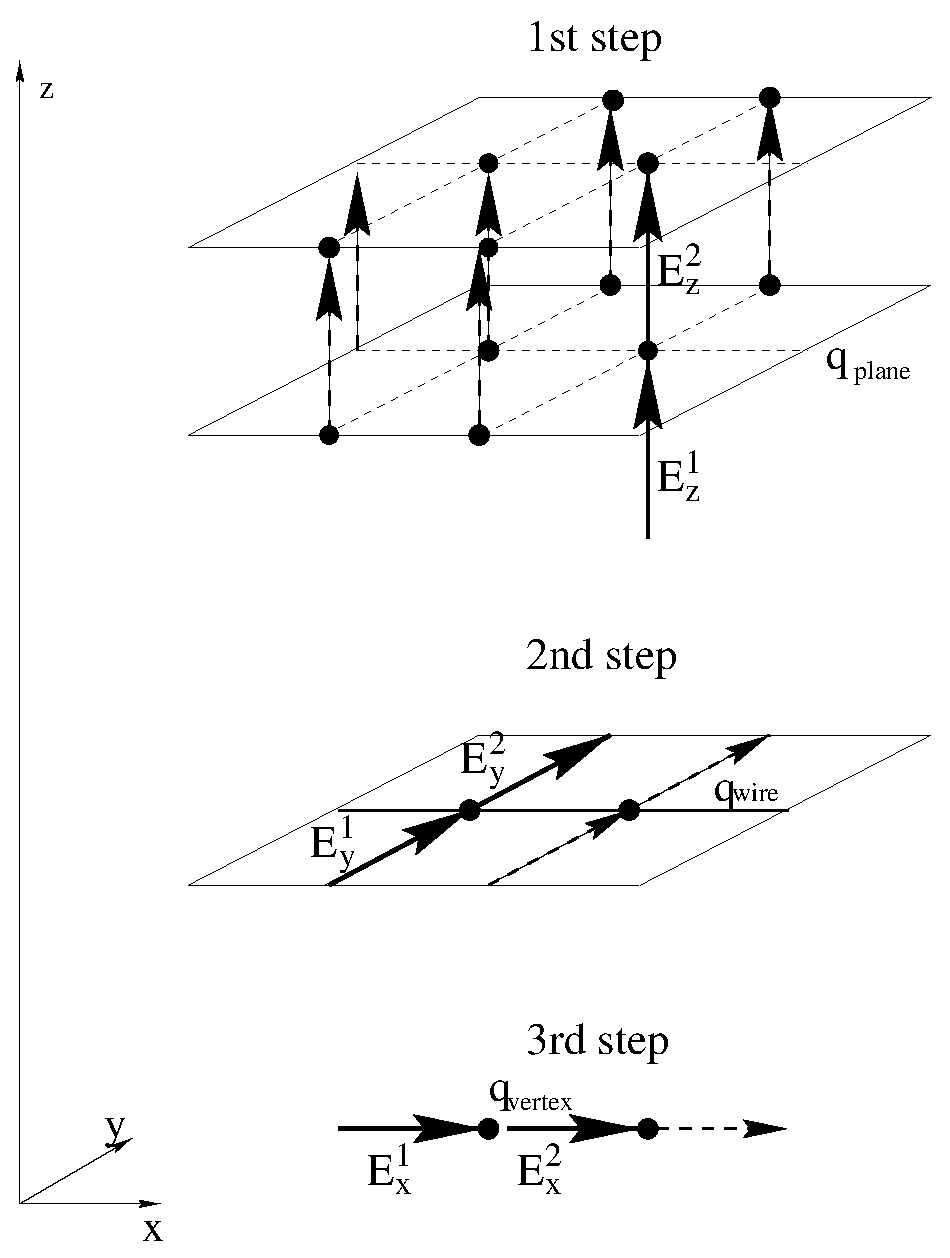
\includegraphics[scale=0.74]{figs/initializationE.eps}
 \caption{Recursive solution of Gauss' law} 
 \label{fig:initialization_E} 
\end{figure} 

%
\section{Time integrator}
%
For the time discretization we have adopted the elegant solution which was found by
Rottler and Maggs \cite{maggs_prl_1} and allows to conserve {\em both}
time--reversibility and phase--space volume conservation:

\begin{enumerate}
\item Update the particle momenta by half a time step.
\item Update the $\vect B$ field by half a time step.
\item Update the particle positions in $x$ direction by half a time step.
\item Update the electric field in $x$ direction by half a time step.
\item Update the particle positions in $y$ direction by half a time step.
\item Update the electric field in $y$ direction by half a time step.
\item Update the particle positions in $z$ direction by half a time step.
\item Update the electric field in $z$ direction by a full time step.
\item Update the particle positions in $z$ direction by half a time step.
\item Update the electric field in $y$ direction by half a time step.
\item Update the particle positions in $y$ direction by half a time step.
\item Update the electric field in $x$ direction by half a time step.
\item Update the particle positions in $x$ direction by half a time step.
\item Update the $\vect B$ field by half a time step.
\item Update the particle momenta by half a time step.
\end{enumerate}
%
\section{Self--energy}
%
The interpolation of the charges onto the lattice gives rise to the
artificial force exerted on the particle by its own field. In order to
cure this remedy, the direct subtraction of the self--energy is introduced.

For the interpolated charge cloud the self--energy can be directly
calculated (see Ref.\cite{phd_pasichnyk}). For the simple cubic
lattice in three dimensions the linear interpolation will give 8
charges which are placed at the corners of the cube with edge length
$a$ (see Fig.~\ref{fig:charge_assig_cubic_lattice}).
%
\begin{figure} 
  \centering 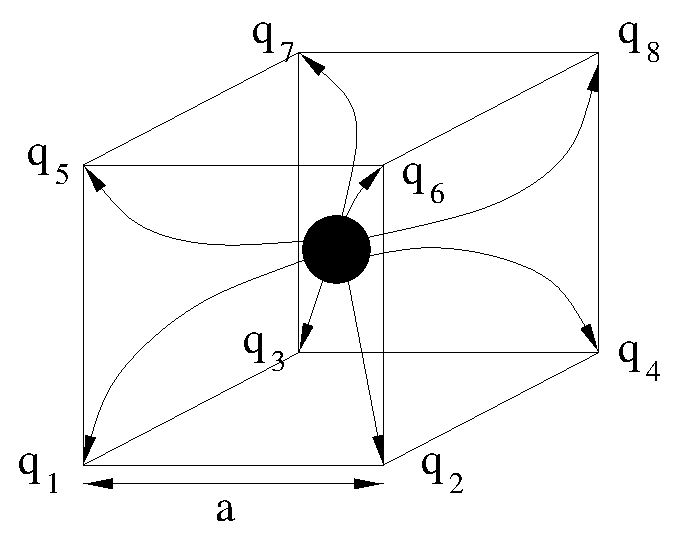
\includegraphics[scale=0.55]{figs/charge_assig_cube.eps}
  \caption{Linear interpolation scheme} 
  \label{fig:charge_assig_cubic_lattice}  
\end{figure}
%
Therefore in our case the self-energy is a symmetric bilinear form
defined by the matrix $\left\{\alpha_{ij}\right\}$, the elements of
which do not depend on the position of the charge. In our algorithm
the values of the coefficients
%
\begin{equation}
  \alpha_{ij}=\frac{1}{4a\epsilon_0L^3}\sum\limits_{\vect k}\frac{\cos \vect k(\vect R_{\imath}-\vect R_{\jmath})}{\sum_{\imath=1}^3(1-\cos\vect
      k\vect a_{\imath})}
\end{equation}
%
where $L$ is tne number of lattice points per dimension, $\vect R_i$ coordinates of the interpolated charges and $\vect k$ the wave vector, are calculated during the initialization step and are used in the
calculation of the self-force. The value of the self-force which has
to be subtracted from the overall forces is given by the following
ansatz
%
\begin{equation}
  \vect F_{self}=-\frac{\partial \mathcal U_{self}}{\partial\vect
    r}=-\sum\limits_i\sum\limits_j\alpha_{ij}\left[q_i\frac{\partial
      q_j}{\partial\vect r}+q_j\frac{\partial q_i}{\partial\vect r}\right].
\end{equation}
%
%
\section{Yukawa screening}
%
Rottler and Maggs \cite{maggs_prl_2} suggest another subtraction
scheme which has the nice property of introducing another optimization
parameter $\kappa$ into the method. Essentially, interactions up to
the length scale $\kappa^{-1}$ are done in real space, while only the
residual long--range part beyond $\kappa^{-1}$ is treated via the
dynamics. A scalar field $\phi$ that couples to the interpolated charges via the energy functional
%
\begin{equation}
{\cal F}\left[\phi\right]= \frac{\epsilon_0}{2} \int d^3 \vect r\left( \vect{\nabla} \phi \right)^2
+ \frac{\epsilon_0}{2} \int d^3 \vect r \kappa^2 \phi^2 + \int d^3 \vect r \, \rho \phi
\end{equation}
%
where $\rho$ is the charge density, leads to an effective interaction between particles of the form
%
\begin{equation}
  U_Y(\vect r)=-\frac{q_iq_j}{4\pi\epsilon_0 r}exp(-\kappa r)
\end{equation}
%
In the algorithm the field $\phi$ obeys the equation of motion
%
\begin{equation}
  \frac{1}{c_{\phi}^2}\frac{\partial^2\phi}{\partial t^2}=\nabla^2\phi-\kappa\phi-\rho
\end{equation}
%
where $c_{\phi}$ is another dynamical parameter of dimension velocity. Currently $c_{\phi}$ is equal to the speed of light. 

In our algorithm we use Yukawa screening to resolve interparticle
interactions on a local scale, such that larger spacings are
feasible. In the method we subtract the self-energy for both the
screened and the unscreened interaction separately by the respective
exact lattice Green's function.  Finally, the Yukawa potential is
corrected at short distances by adding an extra analytic Yukawa
potential (with opposite sign) to the truncated Lennard--Jones
potential.

\begin{thebibliography}{10}

\bibitem{maggs_prl_1}
Rottler J and Maggs A~C \emph{Local molecular dynamics with coulombic
  interaction} cond-mat/0312438
\bibitem{phd_pasichnyk}
Pasichnyk I \emph{Novel simulation methods for Coulomb and hydrodynamic interactions}, PhD thesis, Mainz, 2004
\bibitem{maggs_prl_2}
Rottler J and Maggs A~C \emph{A Continuum, {$\cal O(N)$} Monte-Carlo algorithm for charged particles}, Journal of Chemical Physics, 120, 3119-3129, 2004
\bibitem{espressowebsite}
See web site http://www.espresso.mpg.de
\end{thebibliography}

\end{document}

% Copyright (C) 2010,2012,2013 The ESPResSo project
% Copyright (C) 2002,2003,2004,2005,2006,2007,2008,2009,2010 
%   Max-Planck-Institute for Polymer Research, Theory Group
%  
% This file is part of ESPResSo.
%   
% ESPResSo is free software: you can redistribute it and/or modify it
% under the terms of the GNU General Public License as published by the
% Free Software Foundation, either version 3 of the License, or (at your
% option) any later version.
%  
% ESPResSo is distributed in the hope that it will be useful, but
% WITHOUT ANY WARRANTY; without even the implied warranty of
% MERCHANTABILITY or FITNESS FOR A PARTICULAR PURPOSE.  See the GNU
% General Public License for more details.
%  
% You should have received a copy of the GNU General Public License
% along with this program.  If not, see <http://www.gnu.org/licenses/>.
%
\chapter{The MMM family of algorithms}
\label{chap:mmm}

\section{Introduction}

\todo{Cleanup: References, mathematics} In the MMM family of
algorithms for the electrostatic interaction, a convergence factor
approach to tackle the conditionally convergent Coulomb sum is used
(even the authors of the original MMM method have no idea what this
acronym stands for). Instead of defining the summation order, one
multiplies each summand by a continuous factor
$c(\beta,r_{ij},n_{klm})$ such that the sum is absolutely convergent
for $\beta>0$, but $c(0,.,.)=1$. The energy is then defined as the
limit $\beta\rightarrow 0$ of the sum, i. e. $\beta$ is an artificial
convergence parameter. For a convergence factor of $e^{-\beta
  n_{klm}^2}$ the limit is the same as the spherical limit, and one
can derive the classical Ewald method quite conveniently through this
approach \citep{smith81a}. To derive the formulas for MMM, one has to
use a different convergence factor, namely
$e^{-\beta|r_{ij}+n_{klm}|}$, which defines the alternative energy

\[ \tilde{E}=\,\frac{1}{2}\lim_{\beta\rightarrow
  0}\sum_{k,l,m}{\sum_{i,j=1}^N}' \frac{q_i q_je^{-\beta|p_{ij} +
    n_{klm}|}} {|p_{ij} + n_{klm}|}
=:\,\frac{1}{2}\lim_{\beta\rightarrow 0}\sum_{i,j=1}^N
q_iq_j\phi_\beta(x_{ij}, y_{ij},z_{ij}). \]

$\phi_\beta$ is given by $ \phi_\beta(x,y,z)=\,\tilde\phi_\beta(x,y,z)
+ \frac{e^{-\beta r}}{r} $ for $(x,y,z)\neq 0$ and
$\phi_\beta(0,0,0)=\,\tilde\phi_\beta(0,0,0)$, where

\[ \tilde\phi_\beta(x,y,z)=\,\sum_{(k,l,m)\neq 0} \frac{e^{-\beta
    r_{klm}}}{r_{klm}}. \]

The limit $\tilde{E}$ exists, but differs for three dimensionally
periodic systems by some multiple of the square of the dipole moment
from the spherical limit as obtained by the Ewald
summation\citep{smith81a}. From the physical point of view the Coulomb
interaction is replaced by a screened Coulomb interaction with
screening length $1/\beta$. $\tilde{E}$ is then the energy in the
limit of infinite screening length. But because of the conditional
convergence of the electrostatic sum, this is not necessarily the same
as the energy of an unscreened system. Since the difference to the
Ewald methods only depends on the dipole moment of the system, the
correction can be calculated easily in linear time and can be ignored
with respect to accuracy as well as to computation time.

For one or two dimensionally systems, however, $\tilde{E}=E$, \ie the
convergence factor approach equals the spherical summation limit of
the Ewald sum, and MMM1D and MMM2D do not require a dipole correction.

Starting from this convergence factor approach, Strebel constructed a
method of computational order $O(N\log N)$, which is called MMM
\citep{strebel99a}. The favourable scaling is obtained, very much like
in the Ewald case, by technical tricks in the calculation of the far
formula.  The far formula has a product decomposition and can be
evaluated hierarchically similarly to the fast multipole methods.

For particles sufficiently separated in the z-axis one can Fourier
transform the potential along both x and y. We obtain the far formula
as

\[ \phi(x,y,z) =\, u_x u_y\sum_{p,q\neq 0} \frac{e^{2\pi f_{pq}z} +
  e^{2\pi f_{pq}(\lambda_z-z)}}{f_{pq} \left(e^{2\pi f_{pq}\lambda_z}
    - 1\right)} e^{2\pi i u_y q y}e^{2\pi i u_x p x} + 2\pi u_x
u_y\left(u_z z^2 - z + \frac{\lambda_z}{6}\right). \]

where $\lambda_{x,y,z}$ are the box dimensions, $ f_{pq} =\,
\sqrt{(u_x p)^2 + (u_y q)^2},\quad f_p =\, u_x p,\quad f_q =\, u_x q
$, $ \omega_p=2\pi u_x p$ and $\omega_q=2\pi u_y q$. The advantage of
this formula is that it allows for a product decomposition into
components of the particles. For example

\[ e^{2\pi f_{pq}z}=e^{2\pi f_{pq}(z_i-z_j)}=e^{2\pi
  f_{pq}z_i}e^{-2\pi f_{pq}z_j} \]

etc. Therefore one just has to calculate the sum over all these
exponentials on the left side and on the right side and multiply them
together, which can be done in $O(N)$ computation time. As can be seen
easily, the convergence of the series is excellent as long as z is
sufficiently large. By symmetry one can choose the coordinate with the
largest distance as z to optimise the convergence. Similar to the
Lekner sum, we need a different formula if all coordinates are small,
i. e. for particles close to each other. For sufficiently small
$u_y\rho$ and $u_xx$ we obtain the near formula as

\[ \begin{array}{rl} \tilde\phi(x,y,z)=\, & 2 u_x
  u_y\sum\limits_{p,q>0} \frac{\cosh(2\pi f_{pq}z)}{f_{pq}
    \left(e^{2\pi f_{pq}\lambda_z} - 1\right)} e^{2\pi i u_y q
    y}e^{2\pi i u_x p x} +\\ & 4u_x\sum\limits_{l,p>0}\left(K_0(2\pi
    u_x p\rho_l) + K_N(2\pi u_x p\rho_{-l})\right)cos(2\pi u_x p x)
  -\\ & 2u_x\sum\limits_{n\ge 1}\frac{b_{2n}}{2n(2n)!}\Re\bigl((2\pi
  u_y (z+iy))^{2n}\bigr) +\\ & u_x\sum\limits_{n\ge
    0}\left(\begin{array}{c}-\frac{1}{2}\\
      n\end{array}\right)\frac{\left( \psi^{(2n)}(1 + u_x x) +
      \psi^{(2n)}(1 - u_x x)\right)}{(2n)!}\rho^{2n} -\\ &
  2\log(4\pi). \end{array} \]

Note that this time we calculate $\tilde{\phi}$ instead of $\phi$, i.
e. we omit the contribution of the primary simulation box. This is
very convenient as it includes the case of self energy and makes
$\tilde{\phi}$ a smooth function. To obtain $\phi$ one has to add the
$1/r$ contribution of the primary box. The self energy is given by

\[ \tilde\phi(0,0,0)=\, 2 u_x u_y\sum\limits_{p,q>0} \frac{1}{f_{pq}
  \left(e^{2\pi f_{pq}\lambda_z} - 1\right)}+
8u_x\sum\limits_{l,p>0}K_N(2\pi u_x\lambda_y p l) + 2 u_x\psi^{(0)}(1)
- 2\log(4\pi). \]

Both the near and far formula are derived using the same convergence
factor approach, and consequently the same singularity in $\beta$ is
obtained. This is important since otherwise the charge neutrality
argument does not hold.

To obtain the $O(N\log N)$ scaling, some algorithm tricks are needed,
which are not used in MMM1D, MMM2D or ELC and are therefore not
discussed here. For details, see \citet{strebel99a}. MMM is not
implemented in \es.

\section{MMM2D}

In the case of periodicity only in the x and y directions, the far
formula looks like

\[ \begin{array}{rl} \phi(x,y,z) = \, & 4 u_x u_y\sum_{p,q>0}
  \frac{e^{-2\pi f_{pq}|z|}} {f_{pq}} \cos(\omega_p x)\cos(\omega_q y)
  +\\ & 2 u_x u_y\left(\sum_{q>0} \frac{e^{-2\pi f_q|z|}}{f_q}
    \cos(\omega_q y) + \sum_{p>0} \frac{e^{-2\pi f_p|z|}}{f_p}
    \cos(\omega_p x)\right) -\\ & 2\pi u_x u_y |z| \end{array} \],

and the near formula is

\[ \begin{array}{rl} \tilde\phi(x,y,z)=\, &
  4u_x\sum_{l,p>0}\left(K_0(\omega_p\rho_l) +
    K_0(\omega_p\rho_{-l})\right)\cos(\omega_p x) -\\ & 2u_x\sum_{n\ge
    1}\frac{b_{2n}}{2n(2n)!} \Re\bigl((2\pi u_y
  (z+iy))^{2n}\bigr)\,+\, \sum_{k=1}^{N_\psi-1}\left(\frac{1}{r_{k}} +
    \frac{1}{r_{-k}}\right) -\\ & u_x\sum_{n\ge
    0}\left(\begin{array}{c}-\frac{1}{2}\\n\end{array}\right)\frac{\left(
      \psi^{(2n)}(N_\psi + u_x x) + \psi^{(2n)}(N_\psi - u_x
      x)\right)}{(2n)!}(u_x\rho)^{2n} -\\ &
  2u_x\log\left(4\pi\frac{u_y}{u_x}\right). \end{array} \]

As said before, the energy obtained from these potentials is equal to
the electrostatic energy obtained by the spherical summation limit.
The deeper reason for this is that in some sense the electrostatic sum
is absolutely convergent \citep{mmm2d}.

The near formula is used for particles with a small distance along the
z axis, for all other particles the far formula is used. Below is
shown, that the far formula can be evaluated much more efficiently,
however, its convergence breaks down for small z distance. To
efficiently implement MMM2D, the layered cell system is required,
which splits up the system in equally sized gaps along the z axis. The
interaction of all particles in a layer S with all particles in the
layers S-1,S,S+1 is calculated using the near formula, for the
particles in layers $1,\dots,S-2$, and in layers $S+2,\dots,N$, the
far formula is used.

The implementation of the near formula is relatively straight forward
and can be treated as any short ranged force is treated using the link
cell algorithm, here in the layered variant. The special functions in
the formula are somewhat demanding, but for the polygamma functions
Taylor series can be achieved, which are implemented in mmm-common.h.
The Bessel functions are calculated using a Chebychev series.

The treatment of the far formula is algorithmically more complicated.
For a particle i in layer $ S_i$, the formula can product decomposed,
as in

\[ \begin{array}{rl} \sum_{j\in I_S, S < S_i - 1} q_iq_j\frac{e^{-2\pi
      f_{pq}|z_i-z_j|}}{f_{pq}} \cos(\omega_p (x_i -
  x_j))\cos(\omega_q (y_i - y_j)) = \\
  q_i\frac{e^{-2\pi f_{pq}z_i}}{f_{pq}} \cos(\omega_p
  x_i)\cos(\omega_q y_i) \sum_{j\in I_S, S < S_i - 1}q_je^{2\pi
    f_{pq}z_j} \cos(\omega_p x_j)\cos(\omega_q y_j) + \\
  q_i\frac{e^{-2\pi f_{pq}z_i}}{f_{pq}} \cos(\omega_p
  x_i)\sin(\omega_q y_i) \sum_{j\in I_S, S < S_i - 1}q_je^{2\pi
    f_{pq}z_j} \cos(\omega_p x_j)\sin(\omega_q y_j) + \\
  q_i\frac{e^{-2\pi f_{pq}z_i}}{f_{pq}} \sin(\omega_p
  x_i)\cos(\omega_q y_i) \sum_{j\in I_S, S < S_i - 1}q_je^{2\pi
    f_{pq}z_j} \sin(\omega_p x_j)\cos(\omega_q y_j) + \\
  q_i\frac{e^{-2\pi f_{pq}z_i}}{f_{pq}} \sin(\omega_p
  x_i)\sin(\omega_q y_i) \sum_{j\in I_S, S < S_i - 1}q_je^{2\pi
    f_{pq}z_j} \sin(\omega_p x_j)\sin(\omega_q y_j). \end{array} \]

This representation has the advantage, that the contributions of the
two particles are decoupled. For all particles j only the eight terms

\[ \xi^{(\pm,s/c,s/c)}_j= q_je^{\pm 2\pi f_{pq}z_j} \sin/\cos(\omega_p
x_j)\sin/\cos(\omega_q y_j) \]

are needed. The upper index describes the sign of the exponential term
and whether sine or cosine is used for $x_j$ and $y_j$ in the obvious
way. These terms can be used for all expressions on the right hand
side of the product decomposition. Moreover it is easy to see from the
addition theorem for the sine function that these terms also can be
used to calculate the force information up to simple prefactors that
depend only on p and q.

Every processor starts with the calculation of the terms
$\xi^{(\pm,s/c,s/c)}_j$ and adds them up in each layer, so that one
obtains

\[ \Xi^{(\pm,s/c,s/c)}_s= \sum_{j\in S_s}\xi^{(\pm,s/c,s/c)}_j. \]

Now we calculate

\[ \Xi^{(l,s/c,s/c)}_s=\sum_{t < s - 1}\Xi^{(+,s/c,s/c)}_t \]

and

\[ \Xi^{(h,s/c,s/c)}_s=\sum_{t > s + 1}\Xi^{(-,s/c,s/c)}_t, \]

which are needed for the evaluation of the product decomposition.
While the bottom processor can calculate $\Xi^{(l,s/c,s/c)}_s$
directly, the other processors are dependent on its results. Therefore
the bottom processor starts with the calculation of its
$\Xi^{(l,s/c,s/c)}_s$ and sends up $\Xi^{(l,s/c,s/c)}_s$ and
$\Xi^{(+,s/c,s/c)}_s$ of its top layer s to the next processor dealing
with the layers above. Simultaneously the top processor starts with
the calculation of the $\Xi^{(h,s/c,s/c)}_s$ and sends them down.
After the communicated has been completed, every processor can use the
$\Xi^{(l/h,s/c,s/c)}_j$ and the $\xi^{(\pm,s/c,s/c)}_j$ to calculate
the force rsp. energy contributions for its particles.

In pseudo code, the far formula algorithm looks like:

\begin{enumerate}
\item for each layer $s=1,\ldots,S$ 
  \begin{enumerate}
  \item $\Xi^{(\pm,s/c,s/c)}_s=0$
  \item for each particle $j$ in layer $s$
    \begin{enumerate}
    \item calculate $\xi^{(\pm,s/c,s/c)}_j$
    \item $\Xi^{(\pm,s/c,s/c)}_s += \xi^{(\pm,s/c,s/c)}_j$
    \end{enumerate}
  \end{enumerate}
\item $\Xi^{(l,s/c,s/c)}_3=\Xi^{(+,s/c,s/c)}_1$
\item for each layer $s=4,\ldots,S$
  \begin{enumerate}
  \item $\Xi^{(l,s/c,s/c)}_s=\Xi^{(l,s/c,s/c)}_{s-1} +
    \Xi^{(+,s/c,s/c)}_{s-2}$
  \end{enumerate}
\item $\Xi^{(l,s/c,s/c)}_{S-2}=\Xi^{(-,s/c,s/c)}_S$
\item for each layer $s=(S-3),...,1$ 
  \begin{enumerate}
  \item $\Xi^{(l,s/c,s/c)}_s=\Xi^{(l,s/c,s/c)}_{s+1} +
    \Xi^{(-,s/c,s/c)}_{s+2}$
  \end{enumerate}
\item for each layer $s=1,...,S$
  \begin{enumerate}
  \item for each particle $j$ in layer $s$ 
    \begin{enumerate}
    \item calculate particle interaction from
      $\xi^{(+,s/c,s/c)}_j\Xi^{(l,s/c,s/c)}_s$ and
      $\xi^{(-,s/c,s/c)}_j\Xi^{(h,s/c,s/c)}_s$
    \end{enumerate}
  \end{enumerate}
\end{enumerate}

For further details, see
\citet{mmm2d,arnold02b,elc}.

\subsection{Dielectric contrast}

A dielectric contrast at the lower and/or upper simulation box
boundary can be included comparatively easy by using image charges.
Apart from the images of the lowest and topmost layer, the image
charges are far enough to be treated by the far formula, and can be
included as starting points in the calculation of the $\Xi$ terms. The
remaining particles from the lowest and topmost layer are treated by
direct summation of the near formula.

This means, that in addition to the algorithm above, one has to only a
few things: during the calculation of the particle and cell blocks
$\xi$ and $\Xi$, one additionally calculates the contributions of the
image charges and puts them either in a separate array or, for the
boundary layers, into two extra $\xi$ cell blocks outside the
simulation box. The entries in the separate array are then added up
over all processors and stored in the $\Xi$-terms of the
lowest/topmost layer. This are all modifications necessary for the far
formula part. In addition to the far formula part, there is an
additional loop over the particles at the boundary to directly
calculate their interactions with their images.  For details, refer to
\citet{icmmm2d}.

\section{MMM1D}

In one dimensionally periodic systems with z being the periodic
coordinate, the far formula looks like

\[ \begin{array}{rl} \phi(\rho,z) &=\, 4 u_z\sum_{p\neq 0}
  K_0(\omega\rho)\cos(\omega z) - 2u_z\log(\frac{\rho}{2\lambda_z}) -
  2u_z\gamma\\ F_\rho(\rho,z) &=\, 8\pi u_z^2\sum_{p\neq 0} p
  K_1(\omega\rho)\cos(\omega z) + \frac{2 u_z}{\rho}\\ F_z(\rho,z)
  &=\, 8\pi u_z^2 \sum_{p\neq 0} pK_0(\omega\rho)\sin(\omega z),
\end{array} \]

the near formula is

\[ \begin{array}{rl} \tilde{\phi}(\rho,z) &=\, -u_z\sum_{n\ge 0}
  \left(\begin{array}{c}-\frac{1}{2}\\n\end{array}\right)
  \frac{\left(\psi^{(2n)}(N_\psi + u_z z) + \psi^{(2n)}(N_\psi - u_z
      z)\right)}{(2n)!}(u_z\rho)^{2n} - 2u_z\gamma + \\
  &\phantom{=\,++}
  \sum_{k=1}^{N_\psi-1}\left(\frac{1}{r_k}+\frac{1}{r_{-k}}\right)\\
  \tilde{F}_\rho(\rho,z) &=\, -u_z^3 \sum_{n\ge 0}
  \left(\begin{array}{c}-\frac{1}{2}\\n\end{array}\right)
  \frac{\left(\psi^{(2n)}(N_\psi + u_z z) + \psi^{(2n)}(N_\psi - u_z
      z)\right)}{(2n)!}(u_z\rho)^{2n-1} + \\ &\phantom{=\,++}
  \sum_{k=1}^{N_\psi-1}\left(\frac{\rho}{r_k^3}+\frac{\rho}{r_{-k}^3}\right)
  \\ \tilde{F}_z(\rho,z) &=\, -u_z^2 \sum_{n\ge 0}
  \left(\begin{array}{c}-\frac{1}{2}\\n\end{array}\right)
  \frac{\left(\psi^{(2n + 1)}(N_\psi + u_z z) + \psi^{(2n + 1)}(N_\psi
      - u_z z)\right)}{(2n)!}(u_z\rho)^{2n} + \\ &\phantom{=\,++}
  \sum_{k=1}^{N_\psi-1}\left(\frac{z+k\lambda_z}{r_k^3}+\frac{z-k\lambda_z}{r_{-k}^3}\right),
\end{array} \]

where $\rho$ denotes the xy-distance of the particles. As for the two
dimensional periodic case, the obtained energy is equal to the one
dimensional Ewald sum. Algorithmically, MMM1D is uninteresting, since
neither the near nor far formula allow a product decomposition or
similar tricks. MMM1D has to be implemented as a simple NxN loop.
However, the formulas can be evaluated efficiently, so that MMM1D can
still be used reasonably for up to 400 particles on a single
processor \citep{mmm1d}.

\section{ELC}

The ELC method differs from the other MMM algorithms in that it is not
an algorithm for the calculation of the electrostatic interaction, but
rather represents a correction term which allows to use any method for
threedimensionally periodic systems with spherical summation order for
twodimensional periodicity. The basic idea is to expand the two
dimensional slab system of height h in the non-periodic z-coordinate
to a system with periodicity in all three dimensions, with a period of
$\lambda_z>h$, which leaves an empty gap of height $\delta=\lambda_z -
h$ above the particles in the simulation box.

Since the electrostatic potential is only finite if the total system
is charge neutral, the additional image layers (those layers above or
below the original slab system) are charge neutral, too. Now let us
consider the n-th image layer which has an offset of $n\lambda_z$ to
the original layer. If $n\lambda_z$ is large enough, each particle of
charge q\_j at position $(x_j,y_j,z_j+n\lambda_z)$ and its replicas in
the xy-plane can be viewed as constituting a homogeneous charged sheet
of charge density $\sigma_j = \frac{q_j}{\lambda_x\lambda_y}$. The
potential of such a charged sheet at distance z is $2\pi \sigma_j
|z|$. Now we consider the contribution from a pair of image layers
located at $\pm n\lambda_z$, n>0 to the energy of a charge q\_i at
position $(x_i,y_i,z_i)$ in the central layer. Since $|z_j - z_i| <
n\lambda_z$, we have $|z_j - z_i + n\lambda_z| = n\lambda_z + z_j -
z_i$ and $|z_j - z_i - n\lambda_z|= n\lambda_z - z_j + z_i$, and hence
the interaction energy from those two image layers with the charge
$q_i$ vanishes by charge neutrality:

\[ 2\pi q_i \sum_{j=1}^N \sigma_j(|z_j - z_i + n\lambda_z| + |z_j -
z_i - n\lambda_z|) = 4\pi q_i n\lambda_z \sum_{j=1}^N \sigma_j = 0. \]

The only errors occurring are those coming from the approximation of
assuming homogeneously charged, infinite sheets instead of discrete
charges. This assumption should become better when increasing the
distance $n\lambda_z$ from the central layer.

However, in a naive implementation, even large gap sizes will result
in large errors. This is due to the order of summation for the
standard Ewald sum, which is spherical, while the above approach
orders the cells in layers, called slab--wise summation. Smith has
shown that by adding to the Ewald energy the term

\[ E_c=2\pi M_z^2 - \frac{2\pi M^2}{3}, \]

where M is the total dipole moment, one obtains the result of a
slab--wise summation instead of the spherical limit \citep{smith81a}.
Although this is a major change in the summation order, the difference
is a very simple term. In fact, Smith shows that changes of the
summation order always result in a difference that depends only on the
total dipole moment.

Using the far formula of MMM2D, one can calculate the contributions of
the additional layers up to arbitrarily precision, even for small gap
sizes. This method is called electrostatic layer correction, ELC. The
advantage of this approach is that for the image layers, z is
necessarily large enough, so that all interactions can be represented
using the product decomposition. This allows for an order N evaluation
of the ELC term.

The electrostatic layer correction term is given by

\[ E_{lc}=\sum_{i,j=1}^Nq_iq_j\psi(p_i-p_j), \]

where

\[ \begin{array}{rl} \psi(x,y,z)=&4u_xu_y\sum_{p,q>0}\frac{\cosh(2\pi
    f_{pq}z)}{f_{pq}(e^{2\pi f_{pq}\lambda_z} - 1)} \cos(\omega_p
  x)\cos(\omega_q y) + \\ &2u_xu_y\sum_{p>0}\frac{\cosh(2\pi f_p
    z)}{f_p(e^{2\pi f_p\lambda_z} - 1)}\cos(\omega_p x)+\\
  &2u_xu_y\sum_{q>0}\frac{\cosh(2\pi f_q z)}{f_q(e^{2\pi f_q\lambda_z}
    - 1)}\cos(\omega_q y). \end{array} \]

The implementation is very similar to MMM2d, except that the
separation between slices closeby, and above and below is not
necessary.

\section{Errors}


Common to all algorithms of the MMM family is that accuracy is cheap
with respect to computation time. More precisely, the maximal pairwise
error, i.e. the maximal error of the $\psi$ expression, decreases
exponentially with the cutoffs. In turn, the computation time grows
logarithmically with the accuracy. This is quite in contrast to the
Ewald methods, for which decreasing the error bound can lead to
excessive computation time. For example, P3M cannot reach precisions
above $10^{-5}$ in general. The precise form of the error estimates is
of little importance here, for details see \citet{elc}.

One important aspect is that the error estimates are also exponential
in the non-periodic coordinate. Since the number of closeby and far
away particles is different for particles near the border and in the
center of the system, the error distribution is highly
non--homogenous. This is unproblematic as long as the maximal error is
really much smaller than the thermal energy. However, one cannot
interpret the error simply as an additional error source.

\begin{figure}[ht]
  \centering
  \includegraphics[width=0.4\textwidth]{figures/elc-errordist}
  \caption{Error distribution of the ELC method.}
  \label{fig:ELC-error}
\end{figure}

Figure \ref{fig:ELC-error} shows the error distribution of the ELC
method for a gap size of $10\%$ of the total system height. For MMM2D
and MMM1D the error distribution is less homogenous, however, also
here it is always better to have some extra precision, especially
since it is computationally cheap.


%%% Local Variables: 
%%% mode: latex
%%% TeX-master: "ug"
%%% End: 


\bibliographystyle{plainnat}
\bibliography{bibliography}

\printindex

\end{document}
%%% Local Variables: 
%%% mode: latex
%%% TeX-master: t
%%% End: 
